\chapter{Experimental apparatus: the LHC and the CMS detector\label{sec:experiment}}

The Large Hadron Collider (LHC) is currently the world's most powerful particle collider. Constructed by the European Organization for Nuclear Research (CERN) between 1998 and 2008, its goal is to elucidate the electroweak symmetry breaking mechanism and probe physics beyond the Standard Model with the highest collision energies yet attained.

The research described in this dissertation was conducted on data collected from 8-TeV proton-proton collisions in the LHC by the Compact Muon Solenoid (CMS) detector. This chapter presents a brief overview of the LHC, followed by a description of the CMS detector, its component subsystems, and its data acquisition system.

\section{Large Hadron Collider\label{sec:lhc}}

The Large Hadron Collider (see~\cite{1748-0221-3-08-S08001} for a detailed description) is a circular accelerator and collider of high-energy particles, straddling the French-Swiss border near Geneva, Switzerland. This synchrotron consists of 2 rings for counter-circulating proton or ion beams, 27 km in circumference and located at depths as low as 175 m underground in the tunnel previously occupied by the LEP collider ring.

A system of 1,232 superconducting dipole magnets, cooled to temperatures below 2 K with superfluid helium and generating magnetic fields above 8 T, steer the two particle beams (either protons or lead ions) along their trajectory through the accelerator ring; each dipole magnet has a twin-bore design with two apertures that allow both beams to pass through. Quadrupole magnets are used at various points along the ring to keep the beams focused and reduce dispersion, and also at four interaction points (IPs) to cause the beams to intersect and collide. These interaction points are where the ATLAS, CMS, LHCb, and ALICE detectors are located.

\begin{figure}[hbtp]
  \begin{center}
    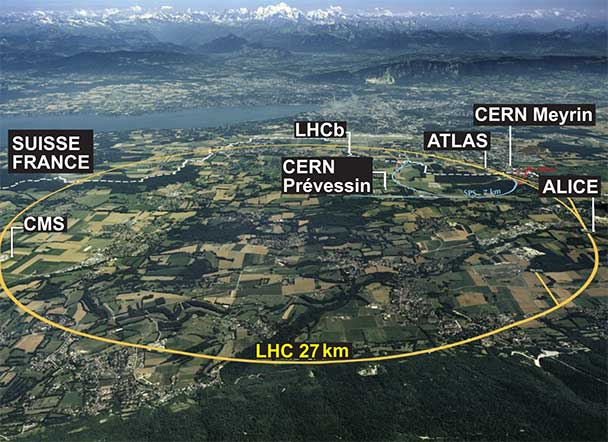
\includegraphics[width=2.0\cmsFigWidth]{figures/lhcring}
    \caption{Aerial view of the Swiss-French border near Geneva, with the path of the LHC ring superimposed~\cite{LHCring}.}
    \label{fig:lhc}
  \end{center}
\end{figure}

Protons, obtained by ionizing hydrogen gas, are accelerated first via a linear accelerator to a kinetic energy of 50 MeV and injected into the Proton Synchrotron Booster, which accelerates them to 1.4 GeV. From there, they are injected into the Proton Synchrotron, which accelerates them further to 25 GeV, and then into the Super Proton Synchrotron, which brings them to an energy of 450 GeV before finally injecting them into the LHC ring, in which they are accelerated to the desired center-of-mass energy for collisions.

Each beam circulating in the LHC contains 2808 bunches of protons, with a bunch spacing of 25 ns. Each bunch has a maximum intensity of 1.15$\cdot$10$^{11}$ protons, limited by the mechanical aperture of the LHC and by the tuning performed to control the linear effects of beam-beam interactions at the collision point.

For a given physics process, the event rate $N$ from a beam collision is given by:

\begin{equation}
N = \mathcal{L}\cdot\sigma_{process}
\label{eq:luminosityxsec}
\end{equation}
where $\mathcal{L}$ is the luminosity of the colliding beams (the number of collisions per unit time per unit cross-sectional area) and $\sigma_{process}$ is the cross-section for the process of interest. The design luminosity of the LHC is driven by the needs of the experiments that take place around its ring.

The LHC is home to several experiments: the general-purpose detectors ATLAS (A Toroidal LHC Apparatus) and CMS (Compact Muon Solenoid), the detector LHCb that focuses on B physics, the detector TOTEM that focuses on elastic proton scattering, and the heavy-ion detector ALICE. The highest luminosity requirements come from ATLAS and CMS, which aim for a peak luminosity of 10$^{34}$ cm$^{-2}$s$^{-1}$; by the logic of Equation~\ref{eq:luminosityxsec}, a high luminosity is needed for obtaining an event rate high enough to be sensitive to Higgs boson production and to rare physics processes beyond the Standard Model.

During a physics run, the collider luminosity progressively decreases, primarily due to beam losses from collisions. Factoring in the effects of all contributions to beam losses, the luminosity has an exponential decay constant of roughly 14.9 h. It is not practical to keep the beams colliding until they have exhausted all their energy, so after a certain point (the optimum run time is around 12 hours), the degraded beams are dumped, so that fresh beams can be generated at peak luminosity to refill the LHC ring.

At peak operation, the total LHC beam current is 0.584A, resulting in a stored energy of 362 MJ. Combined with the total electromagnetic energy of 600 MJ stored in the magnet system, the LHC during operation has a total stored energy of over 1 GJ. All of this energy has to be absorbed safely in a beam dump; this is achieved by a dedicated beam dumping system of magnets to divert the beams out of the ring and thirty-five 24-ton blocks of carbon for absorbing the beams.

The LHC has been designed to collide protons at a maximum center-of-mass energy of 14 TeV. During its first run, it operated at center-of-mass energy 7 TeV from 2010-2012, and then at 8 TeV from 2012-2013. After a long shutdown for planned repairs and maintenance, the LHC was restarted in 2015, operating at 13 TeV, with the intention of eventually increasing to 14 TeV.

\section{Compact Muon Solenoid\label{sec:cms}}

The Compact Muon Solenoid (CMS) detector is a nearly hermetic general-purpose detector at the LHC, gathering data from the collision of proton-proton and heavy ion beams to study a wide range of physics processes. This experiment is characterized by a powerful superconducting solenoid magnet that produces a 4 T magnetic field; the paths of charged particles are deflected by the magnetic field, allowing their momenta and charges to be accurately reconstructed from their trajectories.

When the proton bunches cross at the CMS interaction point, hard scattering interactions between the partons of colliding protons can occur. All the particles produced in such hard scatters pass through and are recorded by a layered system of roughly concentric cylindrical subdetectors. These particles include not only the products of the hard scattering process, but also a lot of extraneous activity as well, such as particles produced via radiation, soft showers coming from partons that do not participate in the hard scattering, and the products of pileup events, which occur when a single bunch crossing results in more than one scattering event~\cite{Sjostrand:2006za}. The CMS detector records the passage of all of these particles, and the data needs to be reconstructed into a picture of the actual event.

The centre of the official CMS coordinate system is at the interaction point, with the x-axis pointing radially inwards towards the centre of the LHC ring and the y-axis pointing vertically upward out of the ground. The radial coordinate in the xy plane is denoted by r, and the azimuthal angle $\phi$ is measured from the x-axis to the y-axis. As a measure of the angle relative to the beam axis (the z-axis), the CMS collaboration uses a quantity called pseudorapidity ($\eta$) instead of $\theta$ because, as the colliding particles travel at speeds comparable to the speed of light, the pseudorapidity converges with a Lorentz-invariant quantity called rapidity $y$:

\begin{equation}
y = \frac{1}{2}\ln(\frac{E+p_{z}}{E-p_{z}})
\label{eq:rapidity}
\end{equation}
The pseudorapidity is defined as:

\begin{equation}
\eta = -\ln[\tan(\frac{\theta}{2})]
\label{eq:pseudorapidity}
\end{equation}
where $\theta$ is the polar angle measured from the z-axis to the xy plane.

The entire detector is a cylindrical structure 21.6 m in length (along the z axis) and 14.6 m in diameter. At the center of the ensemble is a silicon tracker subdetector for reconstructing accurately the momenta of charged particles. Encircling it is the electromagnetic calorimeter (ECAL), a homogenous calorimeter that uses scintillating lead tungstate crystals to reconstruct electrons and photons with high energy resolution. Outside the electromagnetic calorimeter is the hadron calorimeter (HCAL), a sampling calorimeter with alternating layers of brass and scintillator that measures the energy deposited in hadronic showers. The solenoid magnet is located outside the hadronic calorimeter, together with an iron yoke system that provides a return flux for the magnetic field. The outermost layer of the CMS detector is the muon tracking system for identifying and reconstructing the trajectories of muons. Figure~\ref{fig:cms} shows the overall layout of the CMS detector's subsystems.

\begin{figure}[hbtp]
  \begin{center}
    \includegraphics[width=2.0\cmsFigWidth]{figures/wholeCMS3D}
    \caption{Illustration of the various layers of the CMS detector, with a human on the ground to show relative size~\cite{CMSimage}.}
    \label{fig:cms}
  \end{center}
\end{figure}

The solenoid magnet and the various CMS subdetectors will be described in more detail in the rest of this chapter. A more complete description of the CMS detector can be found in~\cite{1748-0221-3-08-S08004}; unless otherwise specified, all information in this chapter is derived from this source.

\subsection{Tracker\label{sec:cms-tracker}}

The tracker detector is the innermost subsystem of the CMS detector. Its purpose is to reconstruct with high resolution the trajectories and momenta of charged particles with transverse momentum 1 GeV and upwards, and to provide high impact parameter resolution for reconstructing the positions of secondary vertices, which are displaced from the point of collision and generally are a characteristic signature of long-lived particles such as those from heavy-flavor processes. Since the tracker detector receives higher irradiation than any other part of the detector due to its proximity to the beam line and the interaction point (IP), the tracker detector has been designed to survive and operate in a high-flux environment, with thousands of particles passing through its volume every 25 ns when the LHC is running at its design luminosity. Thus, the tracker has been designed with these challenges in mind in order to yield good position and time resolution.

The tracker detector is composed of two subdetectors. The one closest to the beam line is the pixel detector; its sensors are 100 $\mu$m $\times$ 150 $\mu$m pixels, which receive an occupancy on the order of $10^{-4}$ per pixel per bunch crossing. The second and larger subdetector is the silicon strip tracker, whose sensors are silicon strips; since it is located at larger radii than the pixel detector, the fluence of particles that reach it is lower and thus the granularity of the silicon strips can be considerably lower than that of the pixel detector, with strip areas ranging from 10 cm $\times$ 80 $\mu$m at intermediate radii for the inner strip tracker (20 $<$ r $<$ 55 cm) and 25 cm $\times$ 180 $\mu$m for the outer strip tracker (55 $<$ r $<$ 110 cm), resulting in an occupancy of about 2-3\% for the inner tracker and 1\% for the outer tracker. These subsystems are illustrated in Figure~\ref{fig:cms-trackerlayout}. The overall envelope of the tracker volume measures 5.8 m in length along the z axis and 2.5 m in diameter.

\begin{figure}[hbtp]
  \begin{center}
    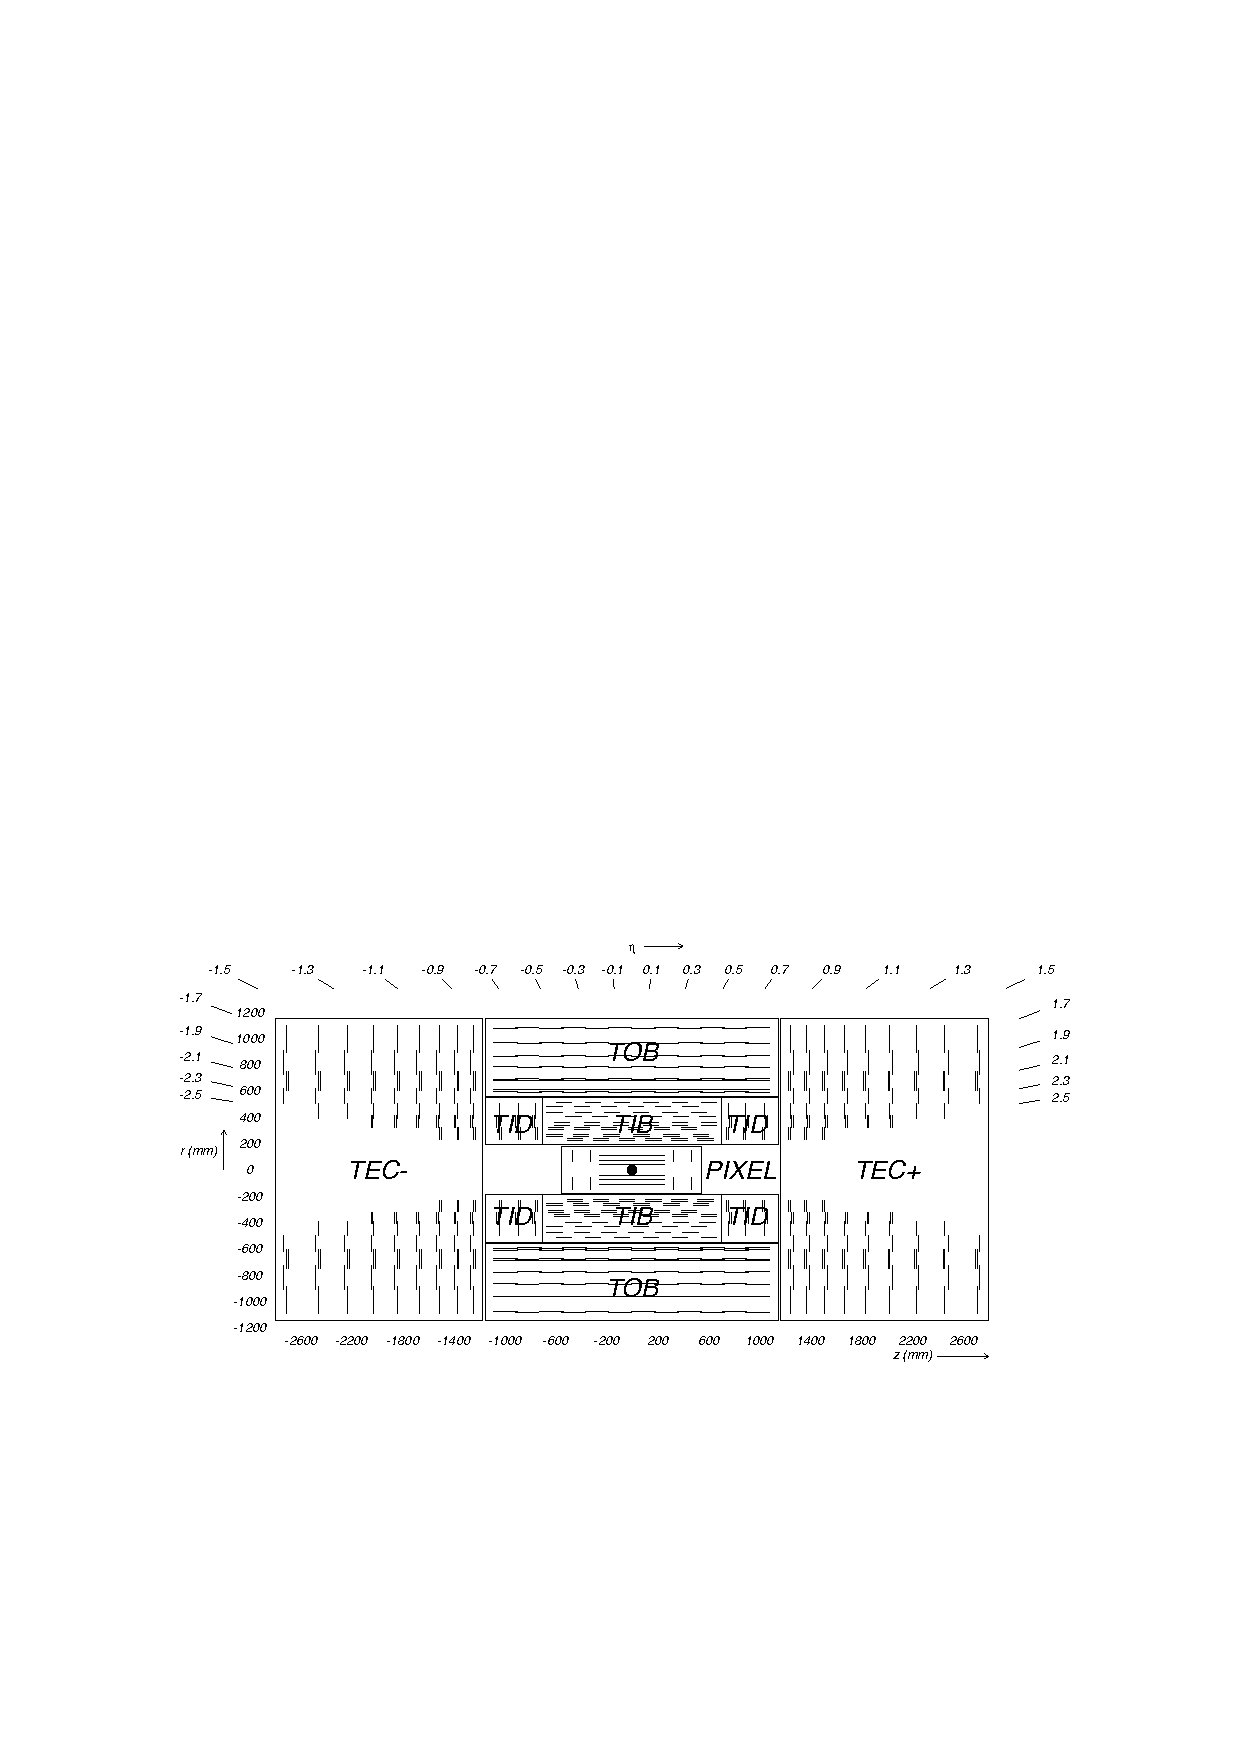
\includegraphics[width=2.0\cmsFigWidth]{figures/cms-trackerlayout}
    \caption{Layout of the CMS tracker detector, showing the pixel detector and the subsystems of the silicon strip tracker; each line represents a detector module~\cite{Dominguez:1481838}.}
    \label{fig:cms-trackerlayout}
  \end{center}
\end{figure}

In total, the CMS tracker detector is comprised of 200 $m^{2}$ of active silicon sensors, providing a coverage of up to $\abs{\eta}$ $<$ 2.5. Because of the high particle fluence passing through the tracker volume during operation, radiation-hard sensors and electronics are required to withstand the radiation dosage; also, an efficient system system of cooling tubes carrying chilled liquid $C_{6}F_{14}$ pervades the tracker volume, keeping it at or below -10 C during operation, thus minimizing radiation damage to the sensors caused either by direct irradiation or by the annealing of radiation-induced defects in the silicon crystal structure through thermal agitation.

\begin{figure}[hbtp]
  \begin{center}
    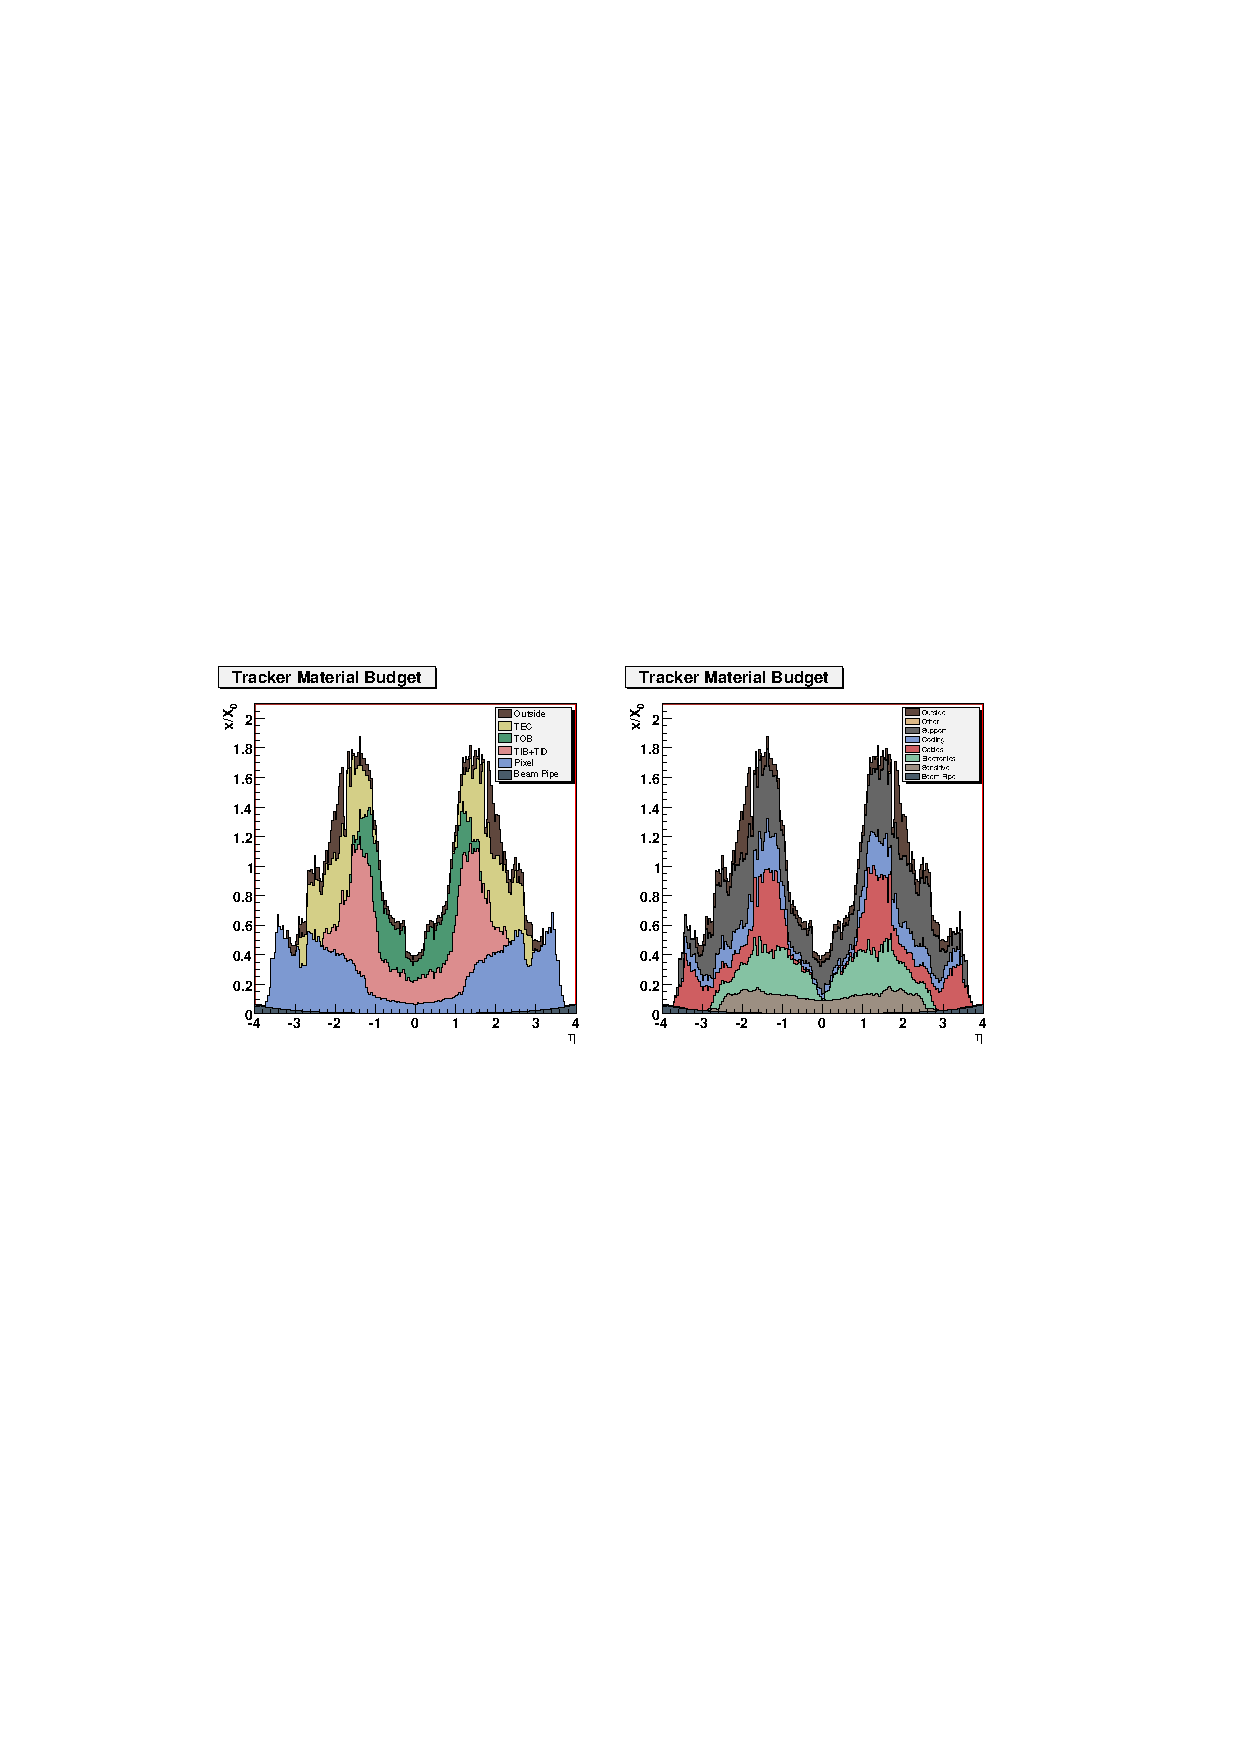
\includegraphics[width=2.4\cmsFigWidth]{figures/cms-tracker-matbudg}
    \caption{Material budget of the tracker detector, displayed in terms of fractional radiation length versus $\eta$, (\cmsLeft) broken down by contribution from the individual subsystems comprising the tracker detector, and (\cmsRight) broken down by contributions from eight different classes of material~\cite{Dominguez:1481838}.}
    \label{fig:cms-tracker-matbudg}
  \end{center}
\end{figure}

Energy loss in the tracker material via multiple scattering, nuclear interactions, gamma conversions, and bremsstrahlung can all interfere with tracking efficiency. Also, bremsstrahlung and gamma conversions in the tracker material will adversely affect the detection and identifcation of electrons and photons in the electromagnetic calorimeter outside the tracker. Thus, the distribution of materials in the tracker, also referred to as the material budget of the tracker, balances  the need for mechanical support for the detector, and the need to minimize the material budget. Figure~\ref{fig:cms-tracker-matbudg} displays the tracker material budget in terms of fractional radiation length as a function of $\eta$, broken down on the one hand by contributions from the individual subdetectors making up the tracker, and on the other hand by contributions from the different categories of material in the tracker volume (outside, support, cooling, cables, electronics, sensitive material, beam pipe, and other). From these plots, it is clear that the material budget of the tracker does not exceed two radiation lengths in any direction.

\subsubsection{Pixel detector\label{sec:cms-pixel}}
% barrel and disks, design of sensors, electronics, readout

The pixel detector is the innermost layer of the tracker detector, with three concentric cylindrical barrel layers complemented by two endcap disks on either side of the interaction point. The barrel layers are located at radii 4.4, 7.3, and 10.2 cm from the beam line, extending out to 2.9 m from the interaction point in the $\pm$z directions. Two endcap disks are located at z $= \pm$34.5 cm and $\pm$46.5 cm, with inner radius 6 cm and outer radius 15 cm. Both the barrel cylinders and endcap disks are split in halves along the y axis for ease of extraction and access.

The pixel sensors consist of 52$\times$80 high-dose $n$-type pixels implanted in a high-resistance $n$-type substrate of 320 $\mu$m thickness on a sensor plate. Each pixel is bump-bonded onto a readout chip (ROC) connected to the sensor plate.

\begin{figure}[hbtp]
  \begin{center}
    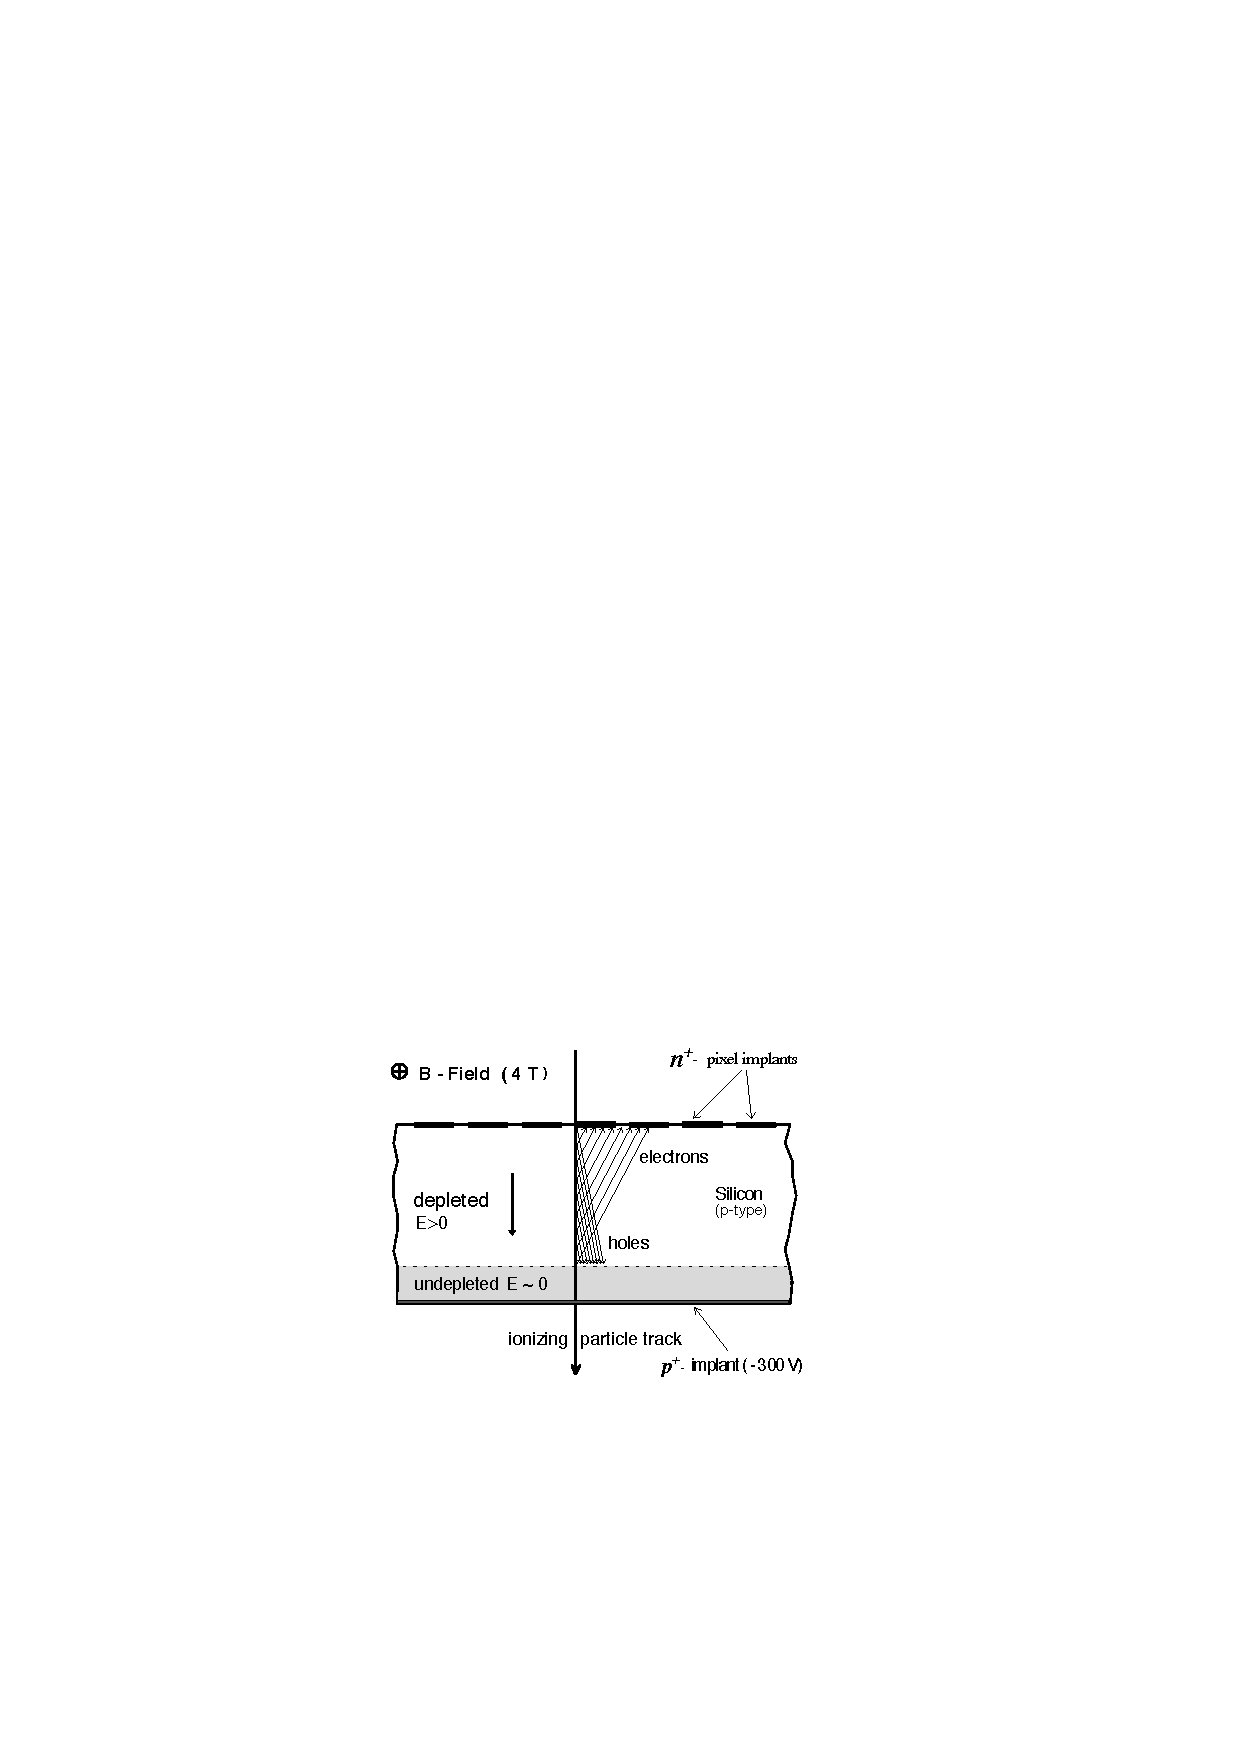
\includegraphics[width=1.24\cmsFigWidth]{figures/cms-pixel-chargesharing}
    \caption{Illustration of charge sharing in a pixel sensor~\cite{Dominguez:1481838}.}
    \label{fig:cms-pixel-chargesharing}
  \end{center}
\end{figure}

When a charged particle passes through a silicon sensor, it induces charge carriers in the n-doped silicon substrate; traveling towards the pixels to be collected, electrons undergo a signficant Lorentz drift (roughly 32$^{\circ}$) due to the 4 T magnetic field along the z axis through the tracker volume, and thus the signal current ends up being spread over adjacent pixels. This process, known as charge sharing, is illustrated in Figure~\ref{fig:cms-pixel-chargesharing}.

The ROC collects and amplifies the analog signals from the pixels, storing them in a buffer until the arrival of the appropriate readout control and clock signals causes it to pass the sensor signal further down the readout system. The analog signal from the ROC is then digitized by the pixel front end digitizer (pxFED) and passed to the CMS data aquisition system for storage. Analog signals above a certain threshold -- to screen out background noise -- are clustered into "hits" by pattern recognition algorithms.

Each pixel sensor has an area of 100 $\mu$m $\times$ 150 $\mu$m. The nearly square design is intended to provide good cluster size and hit resolution in both r$\phi$ and z for the barrel and r$\phi$ and r for the endcaps, as both of these coordinates are needed for measuring track impact parameters. In the barrel, the sensors are arranged 2 $\times$ 8 on rectangular modules (or 1 $\times$ 8 along the edges of the half-cylinders). In each endcap half-disk, the sensors are arranged into groups called plaquettes (there are five different sizes: 1 $\times$ 2, 2 $\times$ 3, 2 $\times$ 4, 1 $\times$ 5, and 2 $\times$ 5), and the plaquettes themselves are arranged into groups of 3 or 4 on a wedge-shaped panel. The panels are mounted onto trapezoidal blades on the endcap disk, with two panels per blade (one on each side); the arrangement of the plaquettes ensures full coverage of the area of the panel. An illustration of the components and shapes of barrel modules and endcap blades can be found in Figure~\ref{fig:cms-pixel-modules}. Altogether, the pixel detector covers a pseudorapidity range of $\abs{\eta}$ $<$ 2.5.

\begin{figure}[hbtp]
  \begin{center}
    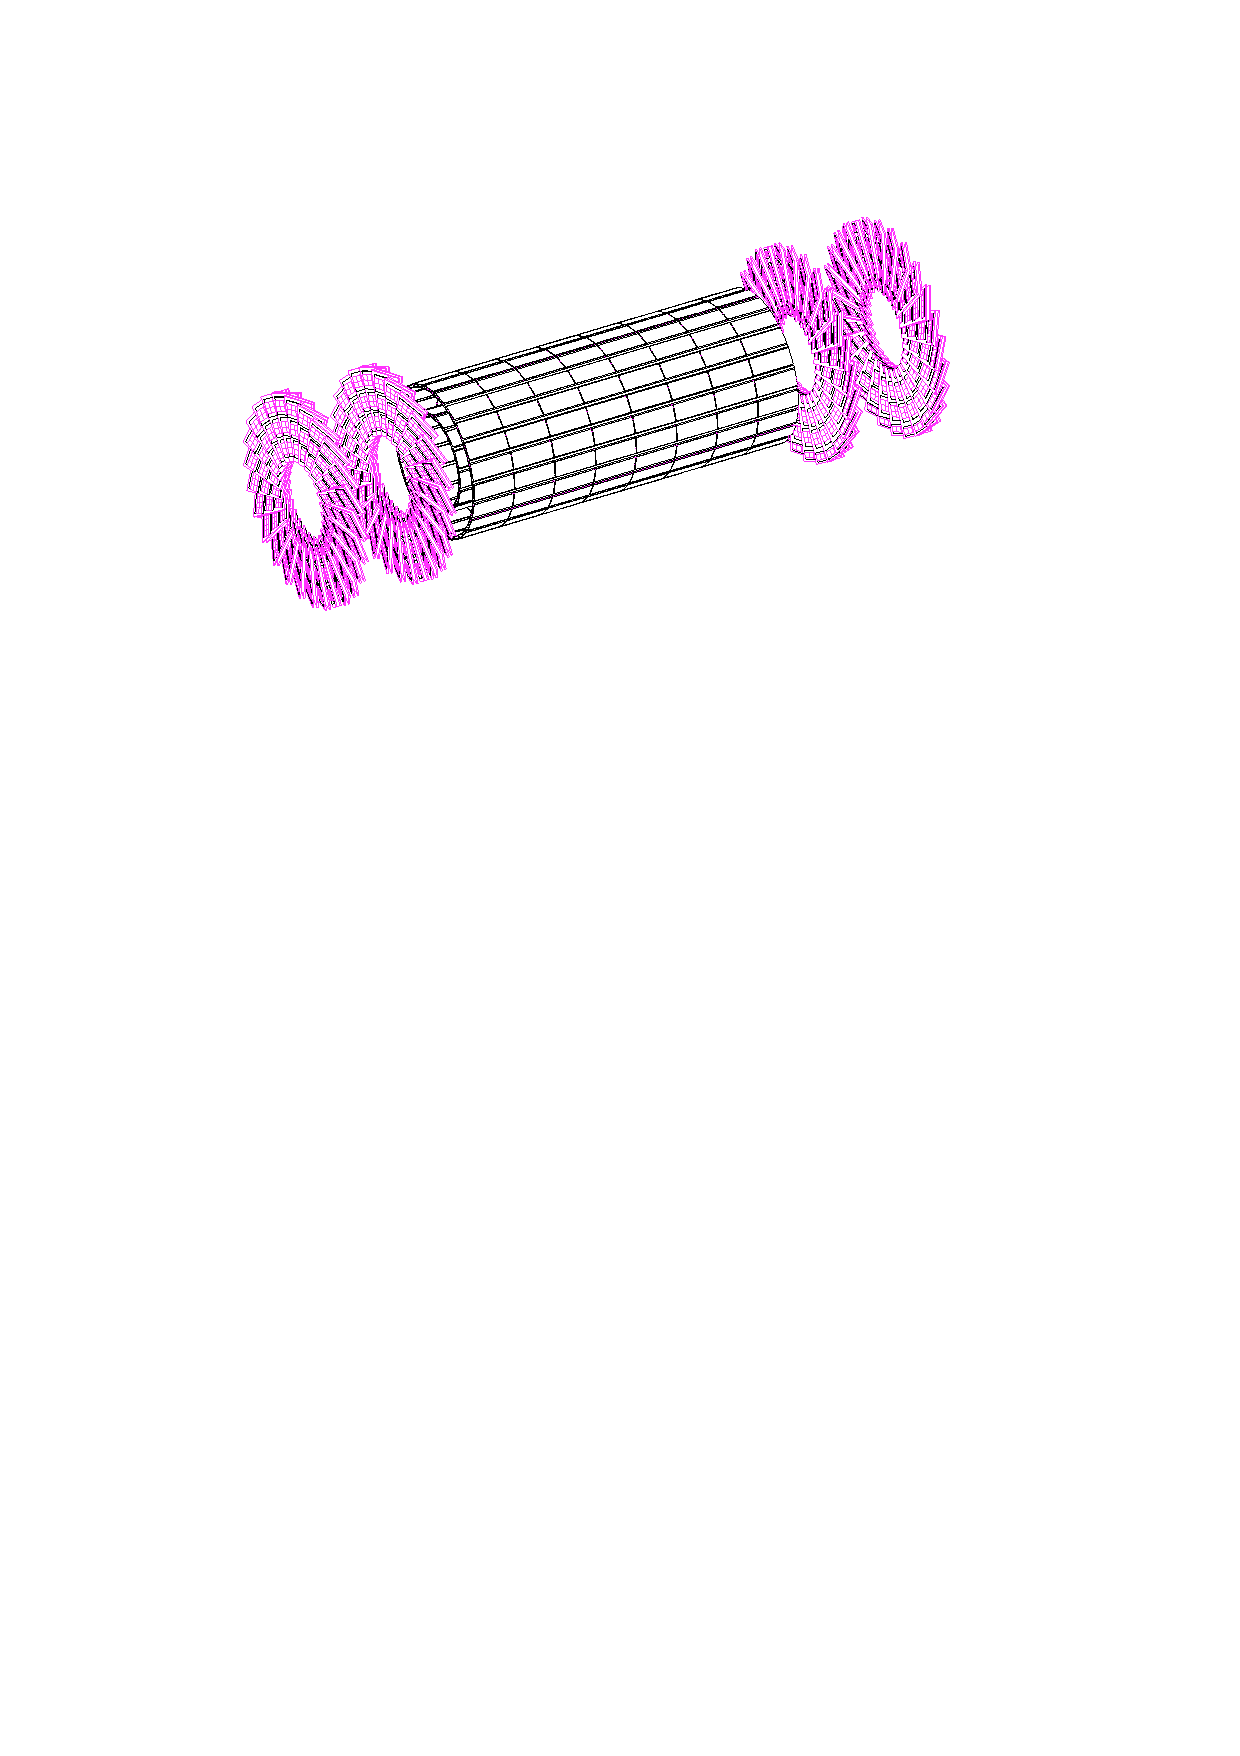
\includegraphics[width=2.0\cmsFigWidth]{figures/cms-pixellayout}
    \caption{Layout of the pixel detector: barrel layers and endcap disks~\cite{Karimaki:368412}. The magenta wedges on the endcap disks are carbon-fibre blades, which hold plaquettes (rectangular arrangements of pixel sensors that come in five different sizes). The black rectangles in the barrel layers are the barrel modules (2$\times$8 rectangular arrangements of pixel sensors), mounted on rectangular carbon-fibre blades.}
    \label{fig:cms-pixellayout}
  \end{center}
\end{figure}

\begin{figure}[hbtp]
  \begin{center}
    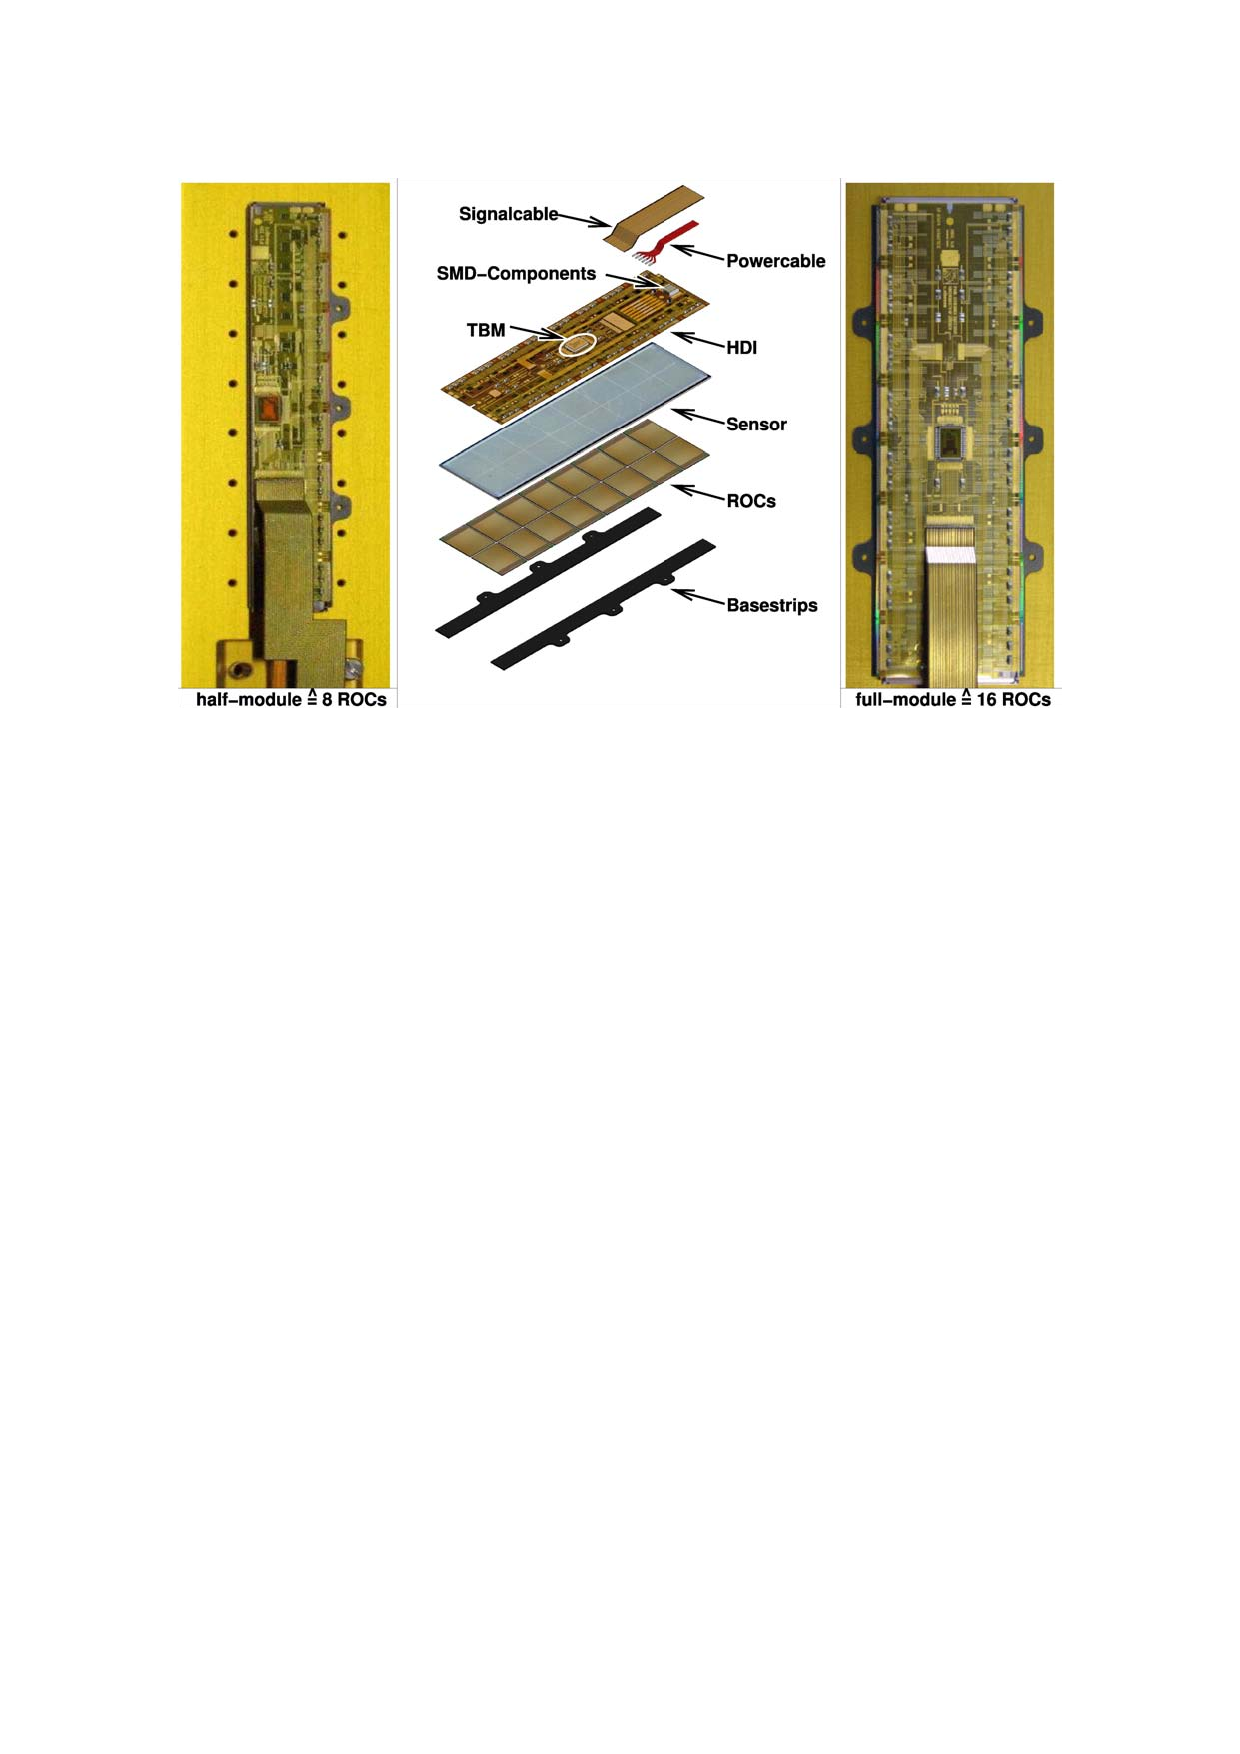
\includegraphics[width=1.5\cmsFigWidth]{figures/cms-pixel-bpixmodule}
    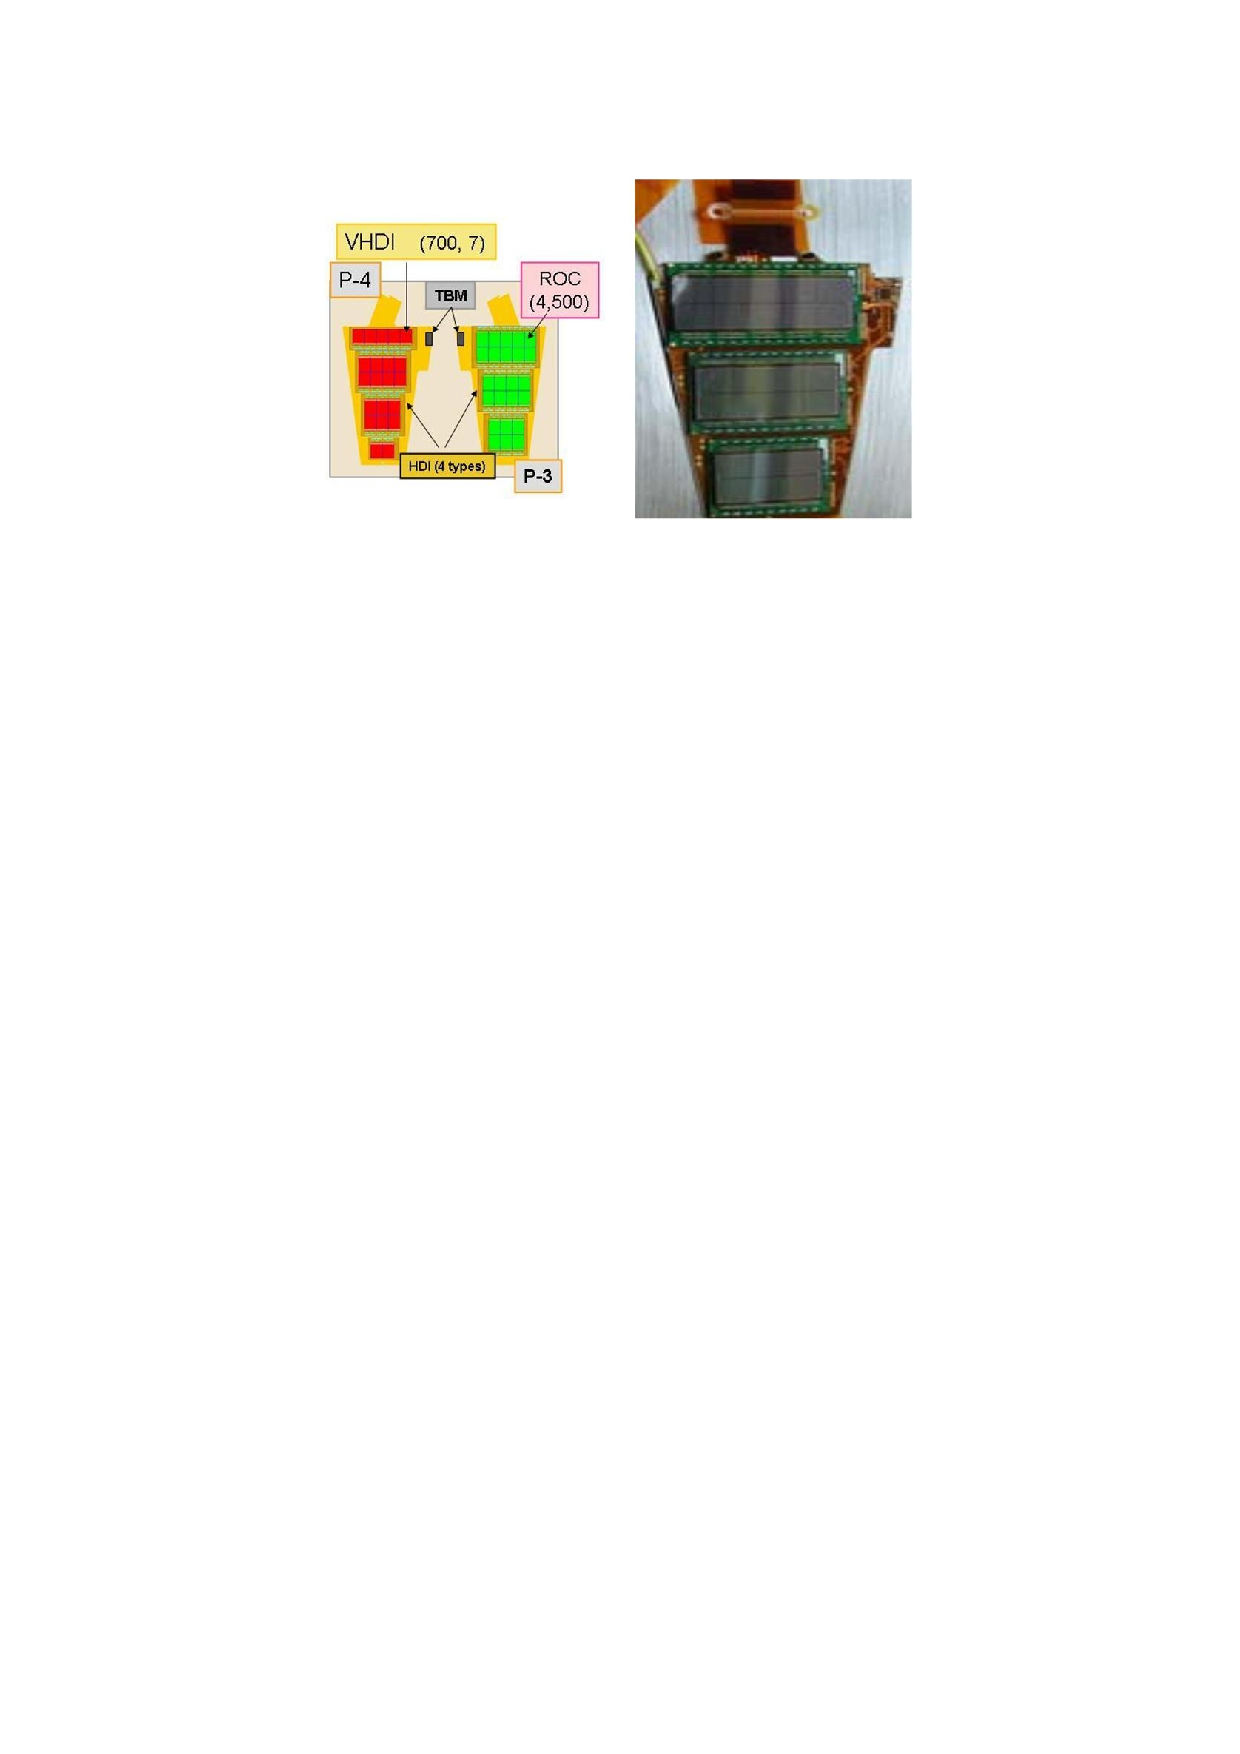
\includegraphics[width=2.0\cmsFigWidth]{figures/cms-pixel-fpixmodule}
    \caption{(Top) Components and shape of a barrel pixel module. (Bottom) Components and shape of an endcap pixel blade, showing the five different plaquette sizes. ~\cite{1748-0221-3-08-S08004}}
    \label{fig:cms-pixel-modules}
  \end{center}
\end{figure}
 
In the barrel, the normal direction of the pixel cells points along the radial direction, perpendicular to the magnetic field, so the Lorentz drift is along the r$\phi$ direction. To induce charge sharing in the pixel endcaps, whose normal points along the magnetic field axis, the blades are rotated at a 20$^{\circ}$ angle about their radial axis in a turbine-like geometry. Hit resolution is improved by interpolating between signals from multiple neighbouring pixels due to charge sharing. All in all, resolutions of 10-20 $\mu$m are achieved in the pixel detector. The hit efficiency of each sensor is the probability of reconstructing a cluster if that sensor has been traversed by a charged particle; Figure~\ref{fig:cms-pixel-performance} shows that the average hit efficiency of each barrel layer and endcap disk, measured in proton-proton collisions at 7 TeV, is well above 90\%.

\begin{figure}[hbtp]
  \begin{center}
    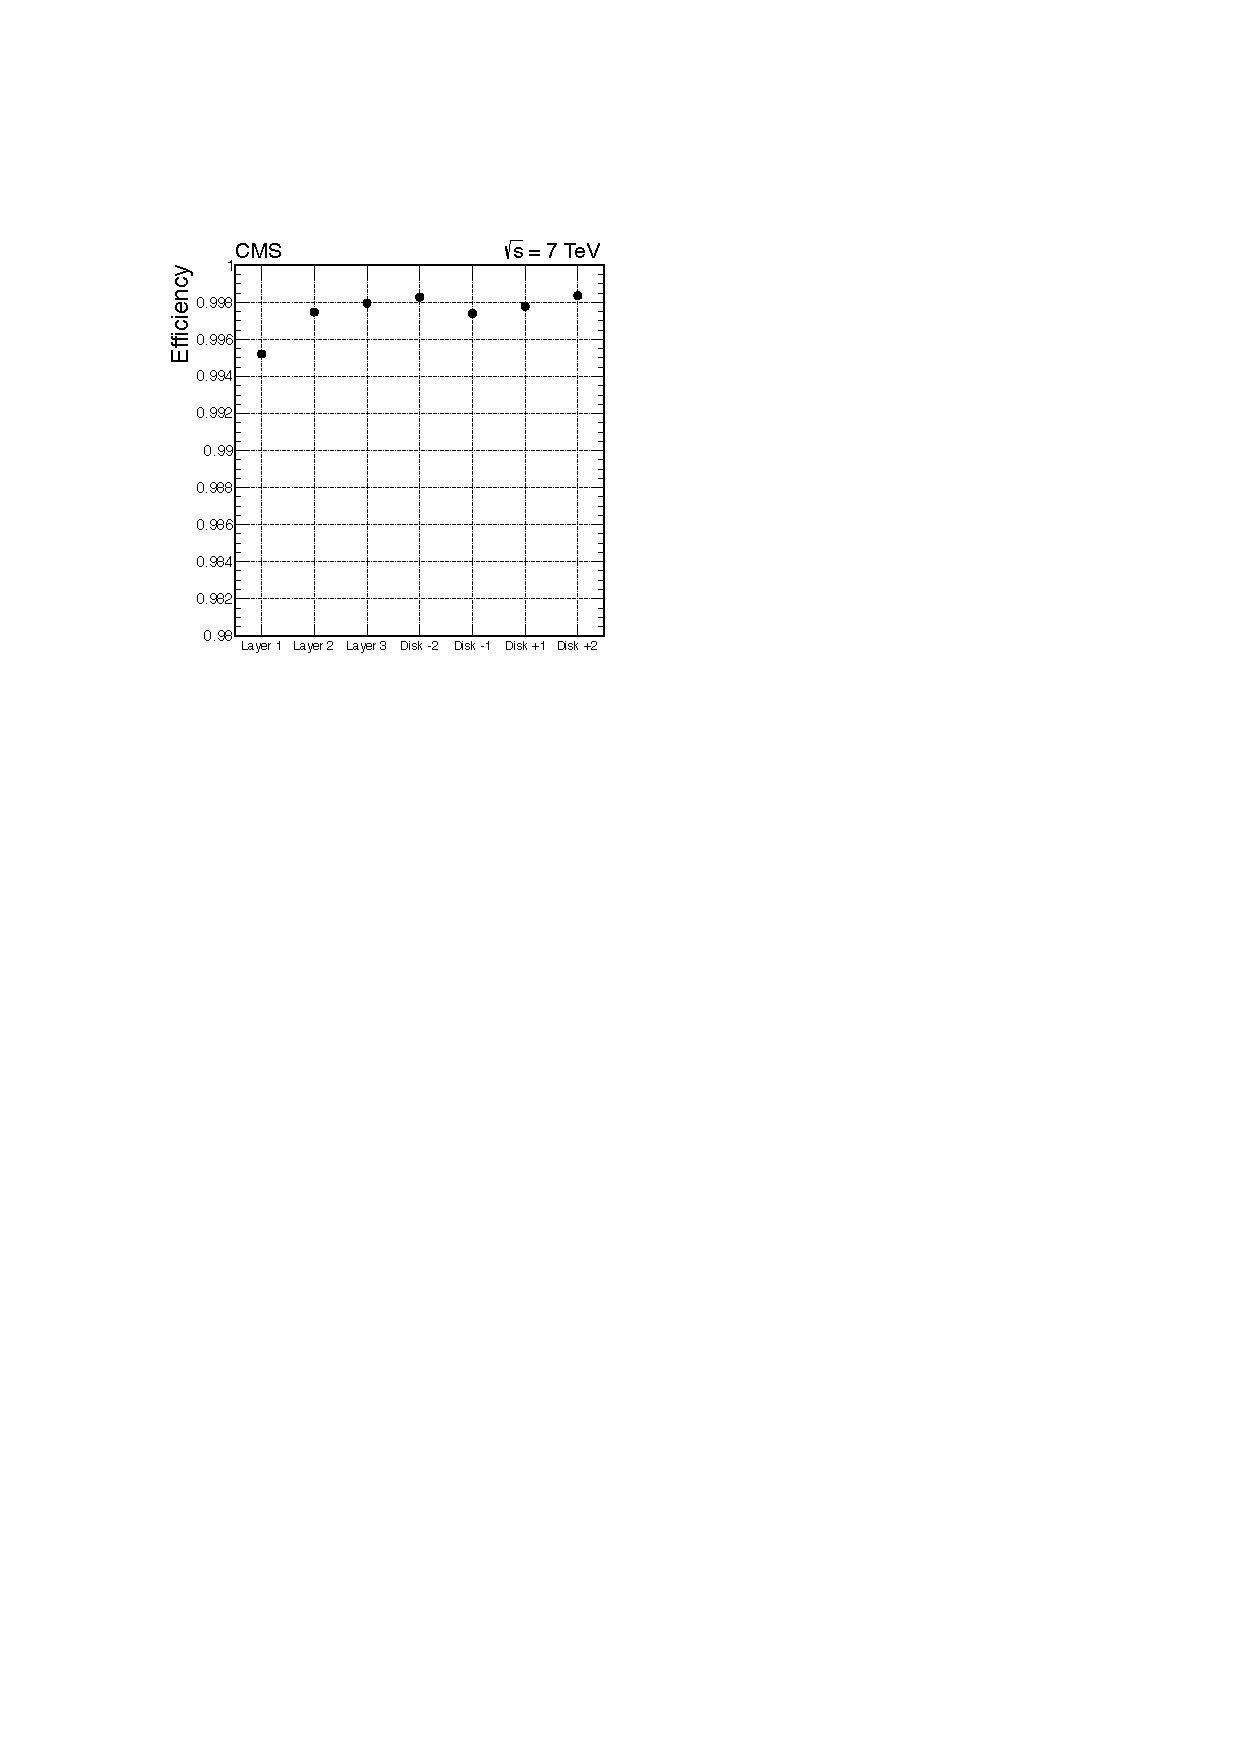
\includegraphics[width=2.0\cmsFigWidth]{figures/cms-pixel-performance}
    \caption{Average hit efficiency in CMS pixel barrel layers and endcap disks, recorded in 7 TeV data from the LHC~\cite{Chatrchyan:2014fea}. Defective modules were excluded from the efficiency calculations.}
    \label{fig:cms-pixel-performance}
  \end{center}
\end{figure}

\subsubsection{Silicon strip detector\label{sec:cms-strips}}
% barrel and disks, design of sensors, electronics, readout

Outside the pixel detector, at $r$ $=$ 20 cm to 116 cm about the beam line and extending 118 cm in the +z and -z directions, lies the silicon strip detector. It is composed of 3 main subsystems: the tracker inner barrel and disks (TIB and TID), the tracker outer barrel (TOB), and the tracker endcaps (TEC).

To optimize coverage, the silicon microstrip sensors in any given barrel layer or endcap disk are positioned to partially overlap with one another, thus resulting in a nonzero pitch with respect to the surface to which they are attached. The silicon strip tracker contains a total of 15,148 modules, each bearing one 320 $\mu$m-thick sensor or two 500 $\mu$m-thick sensors. All in all, there are 29 different module designs, differing in the size of their active area based on the number and size of the sensors. Figure~\ref{fig:cms-tecmodule} shows an example of a module from the TEC, housing two sensors. The silicon microstrip sensors have a single-sided $p$-on-$n$ design. Signal currents are amplified and stored by a custom integrated circuit called an APV25 before being transmitted via optical fibers through the readout system for digitization and storage.

\begin{figure}[hbtp]
  \begin{center}
    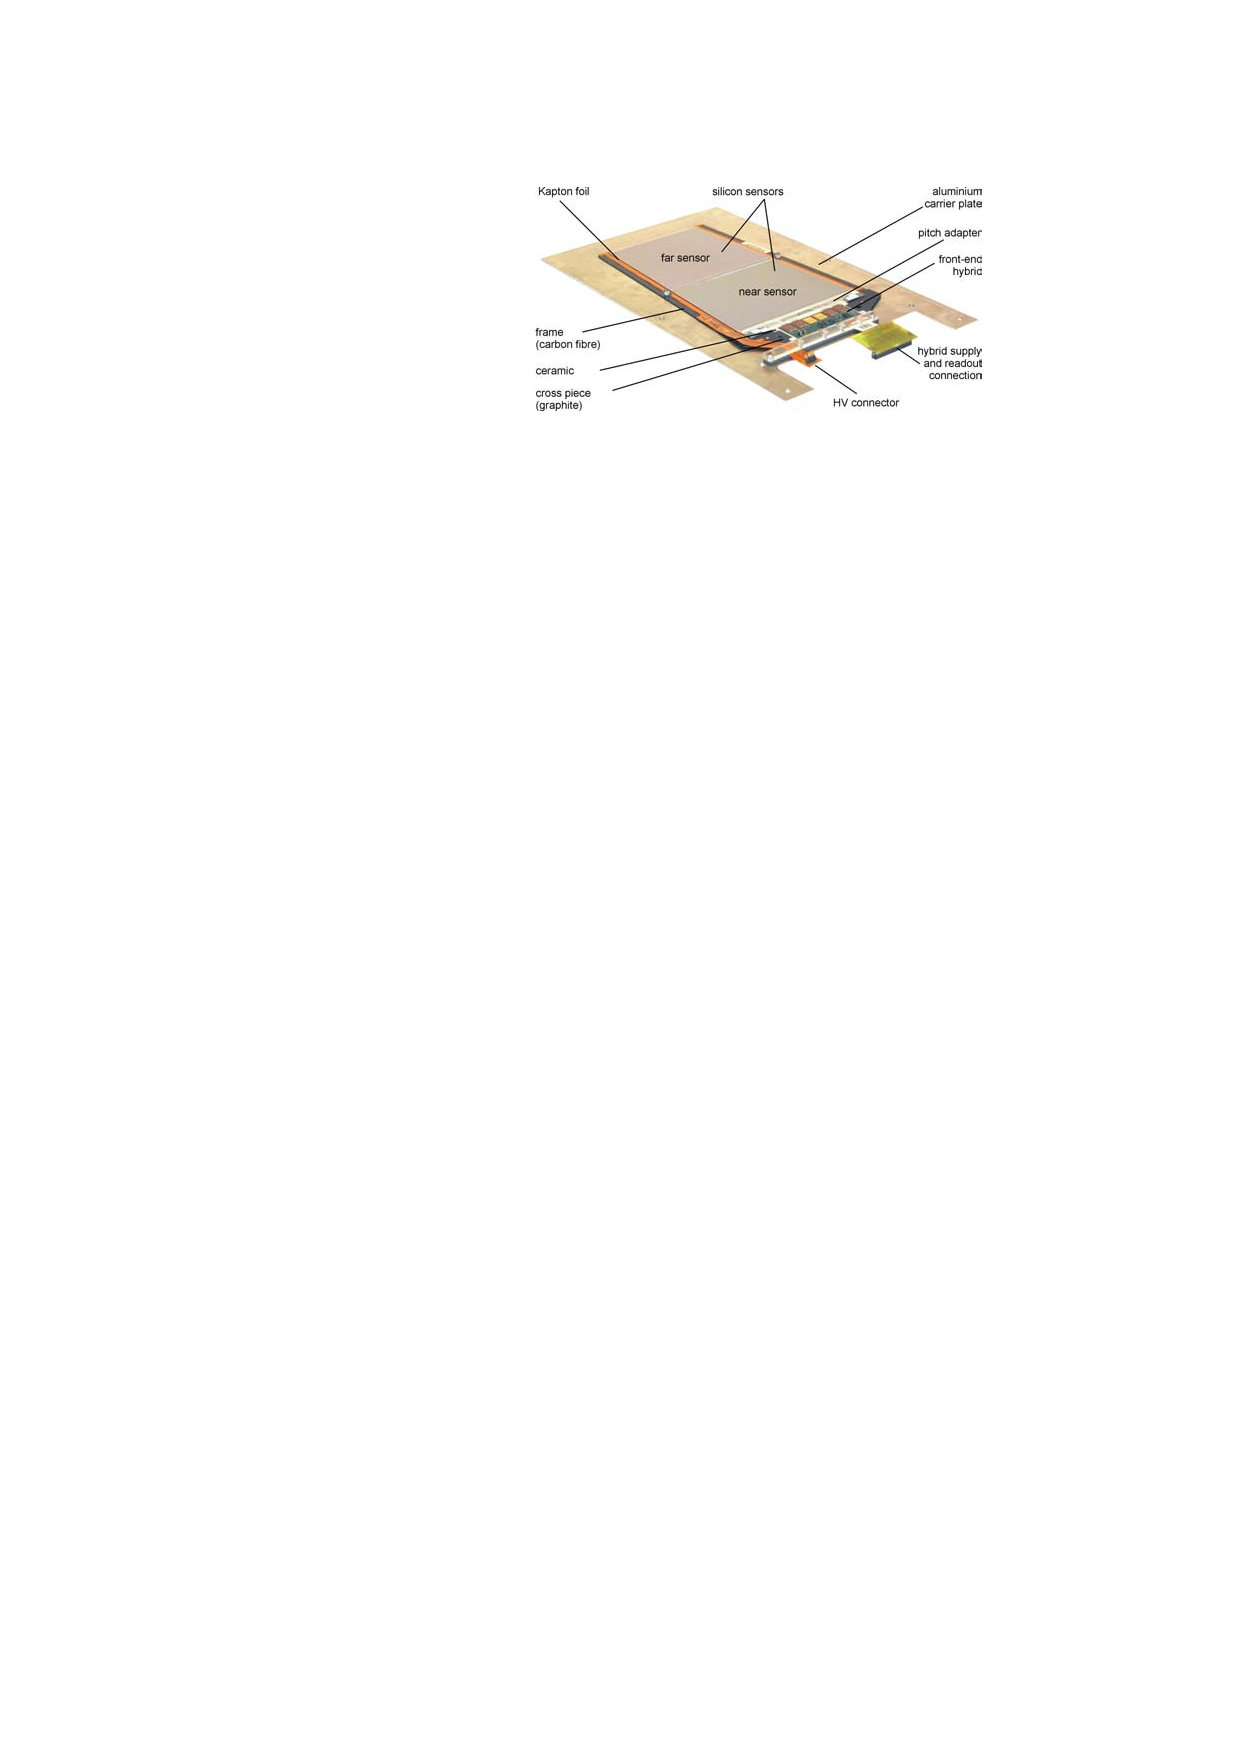
\includegraphics[width=1.24\cmsFigWidth]{figures/cms-tecmodule}
    \caption{Photo of a TEC module, composed of 2 sensors~\cite{1748-0221-3-08-S08004}.}
    \label{fig:cms-tecmodule}
  \end{center}
\end{figure}

The TIB consists of 4 barrel layers 140.0 cm in length, with radii of 255.0 mm, 339.0 mm, 418.5 mm, and 498.0 mm, altogether providing up to 4 r-$\phi$ measurements per particle trajectory. The sensors are silicon microstrips with a thickness of 320 $\mu$m, lying parallel to the beam axis, with a pitch of 80 $\mu$m on the inner two layers and 120 $\mu$m on the outer two layers, yielding a single-point resolution of 23 $\mu$m for the inner two layers and 35 $\mu$m for the outer two layers.

The TID is comprised of six endcap disks, three at each end of the TIB between $\pm$80.0 cm and $\pm$90.0 cm on the z axis; each disk consists of three support rings from $r$ $=$ 200 $\mu$m to 500 $\mu$m. Silicon microstrips, similar to the ones used in the barrel, lie radially on the disks, with a pitch varying from 100 $\mu$m to 141 $\mu$m. While the pixel detector is split down the y axis into half-cylinders for ease of installation, access, and independent testing, the TIB and TID are split into half-shells along the x axis for similar reasons. Two carbon-fibre service cylinders are coupled to the $\pm$z ends of the TIB, providing a route to the TIB shells for service cables originating from a service distribution disk called a margherita, and also housing the TID.

The TOB surrounds the TIB with 6 barrel layers, reaching to an outer radius of 116 cm and spanning 118 cm in the $\pm$z directions. The silicon microstrip sensors here are 500 $\mu$m thick and have a pitch of 183 $\mu$m in the inner four layers and 122 $\mu$m in the outer two layers, yielding a single-point resolution of 53 $\mu$m and 35 $\mu$m respectively in those layers. On either end of the TOB, the TEC extends radially from 220 mm to 1135 mm and in the $\pm$z direction from $\pm$1240 mm to $\pm$2800 mm; each side consists of an assembly of 9 disks with up to 7 rings bearing silicon microstrip sensors, plus 2 extra disks that serve as front-back termination. The microstrip sensors used here have a thickness of 320 $\mu$m in the four rings closest to the TOB and 500 $\mu$m in the remaining outer rings, with a pitch varying from 97 to 184 $\mu$m.

\begin{figure}[hbtp]
  \begin{center}
    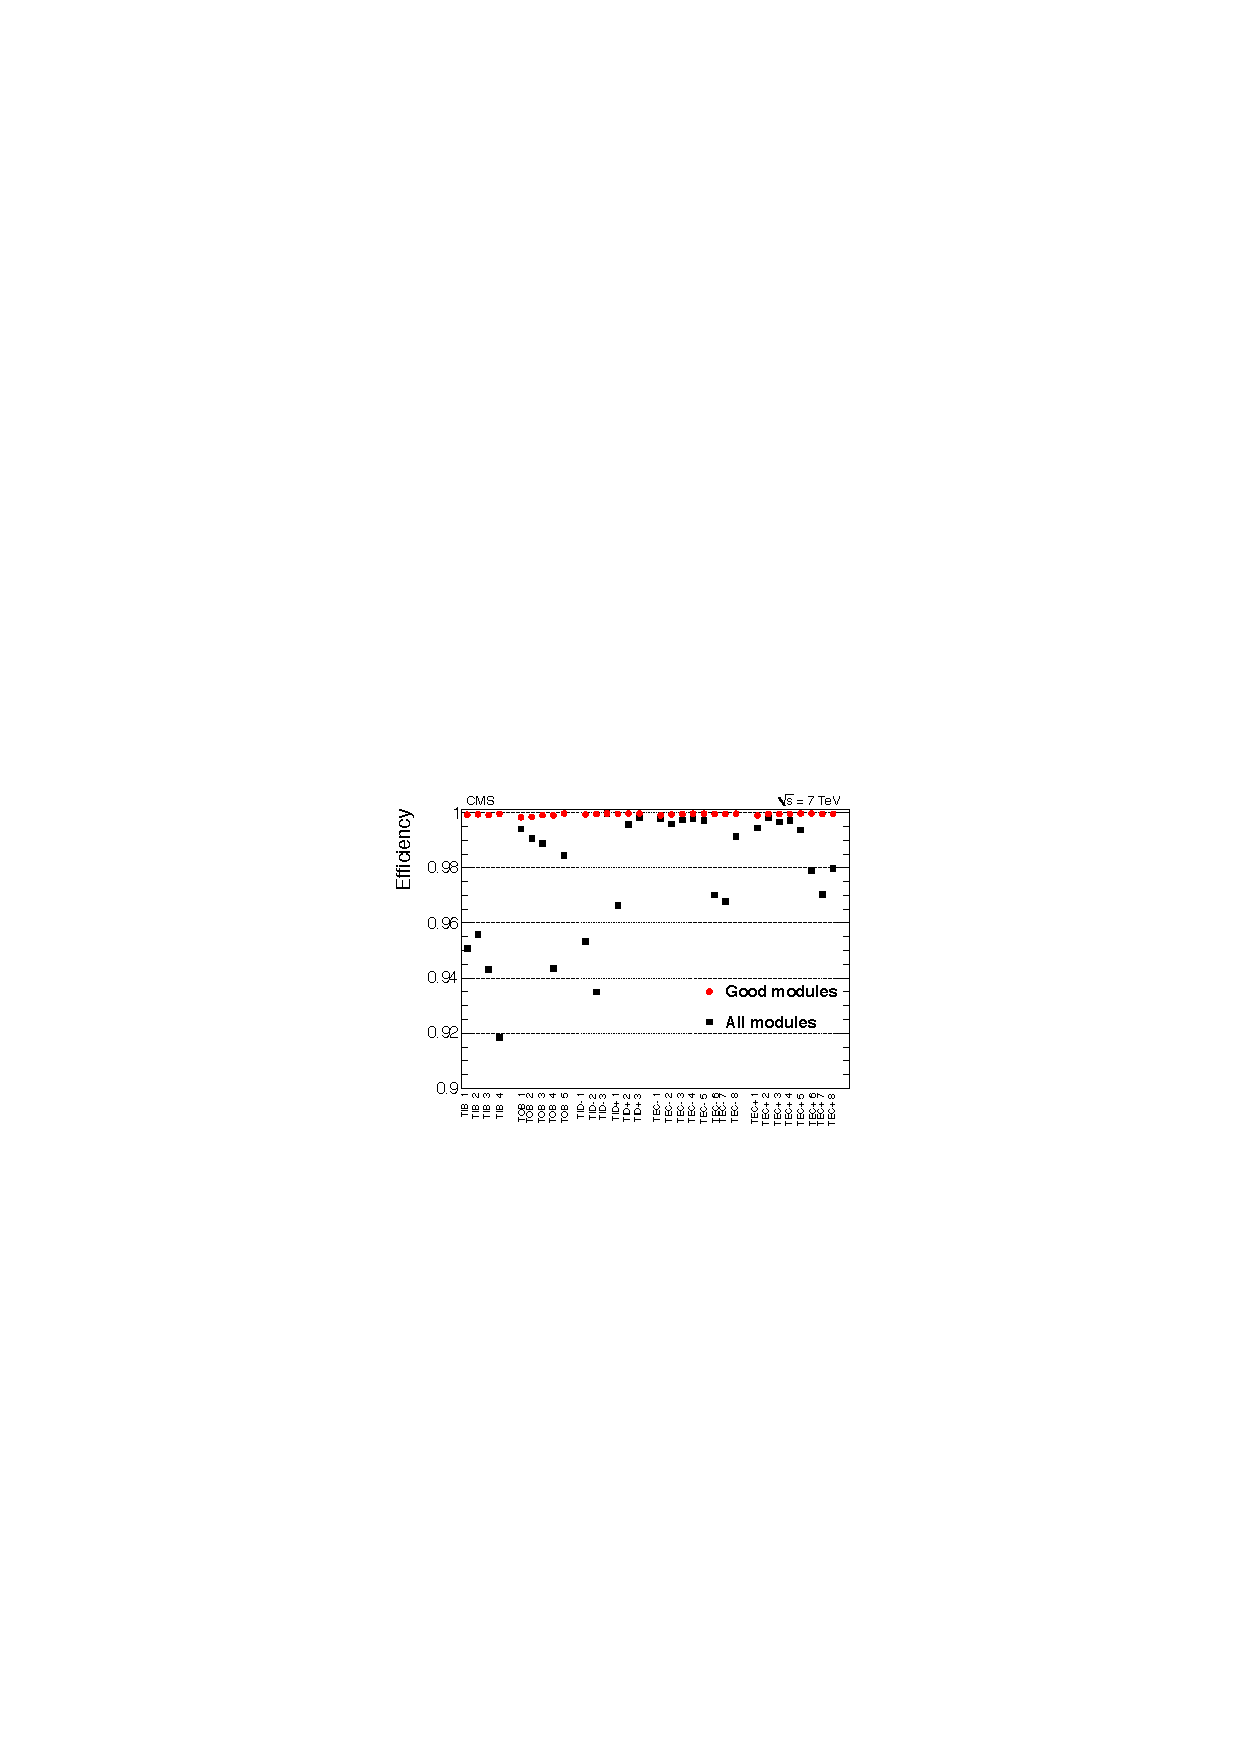
\includegraphics[width=2.0\cmsFigWidth]{figures/cms-strip-performance}
    \caption{Average hit efficiency for the layers and endcap disks of the CMS strip detector, recorded in 7 TeV data from the LHC~\cite{Chatrchyan:2014fea}. The red points are efficiencies measured without considering defective modules, while the black efficiency points were measured with defective modules included.}
    \label{fig:cms-strip-performance}
  \end{center}
\end{figure}

The average hit efficiencies for the various subsystems of the strip detector is shown in Figure~\ref{fig:cms-strip-performance}. These efficiencies are close to 100\%, and even when defective modules are considered, the efficiencies are still above 90\%.

\subsection{Electromagnetic calorimeter\label{sec:cms-ecal}}
% crystals, photodetectors, readout, preshower

One of the primary goals of the CMS experiment is the elucidation of the Higgs mechanism and measurement of the properties of the Higgs boson. The diphoton final state is an important search channel for the Higgs boson, as such a resonance would show up clearly above the background spectrum in the mass range constrained by the latest measurements from the LEP experiment. Other possible search channels include final states involving electrons or positrons, such as $H\rightarrow$$WW/ZZ$. Standard Model measurements and searches for new physics signals can also profit from efficient electron and photon identification. Thus, the need for the CMS detector to provide good photon reconstruction and resolution has driven the optimization of the electromagnetic calorimeter.

The hermetic, homogeneous CMS electromagnetic calorimeter (ECAL) is made up of lead tungstate (PbWO$_4$) crystals. Like the inner tracking system, it is composed of a cylindrical barrel system (with a total of 61,200 crystals) and an endcap system (one endcap disk on each side of the barrel, with 7324 crystals per disk). Its layout is illustrated in Figure~\ref{fig:cms-ecallayout}.

The total thickness of the ECAL is larger than 25 radiation lengths $\chi_0$. When electrons or photons pass through, the resulting electromagnetic showers that they generate excite the scintillator atoms, causing them to emit blue-green scintillation light (up to 420-430 nm in wavelength) that is collected, amplified, and read out by photodetectors glued to the ends of the crystals. Adjacent energy deposits above a background-rejecting threshold are sorted by pattern recognition algorithms into groups called clusters, which may be sorted further into larger agglomerations called superclusters.

High granularity is needed for good energy resolution in the ECAL. The choice of PbWO$_4$, with a density of 8.28 g/cm$^3$, a radiation length of 0.89 cm, and a Moliere radius of 2.2 cm, allows for compact, granular crystals that can resist radiation damage under the high particle fluences that the detector is subjected to throughout its operation.

\begin{figure}[hbtp]
  \begin{center}
    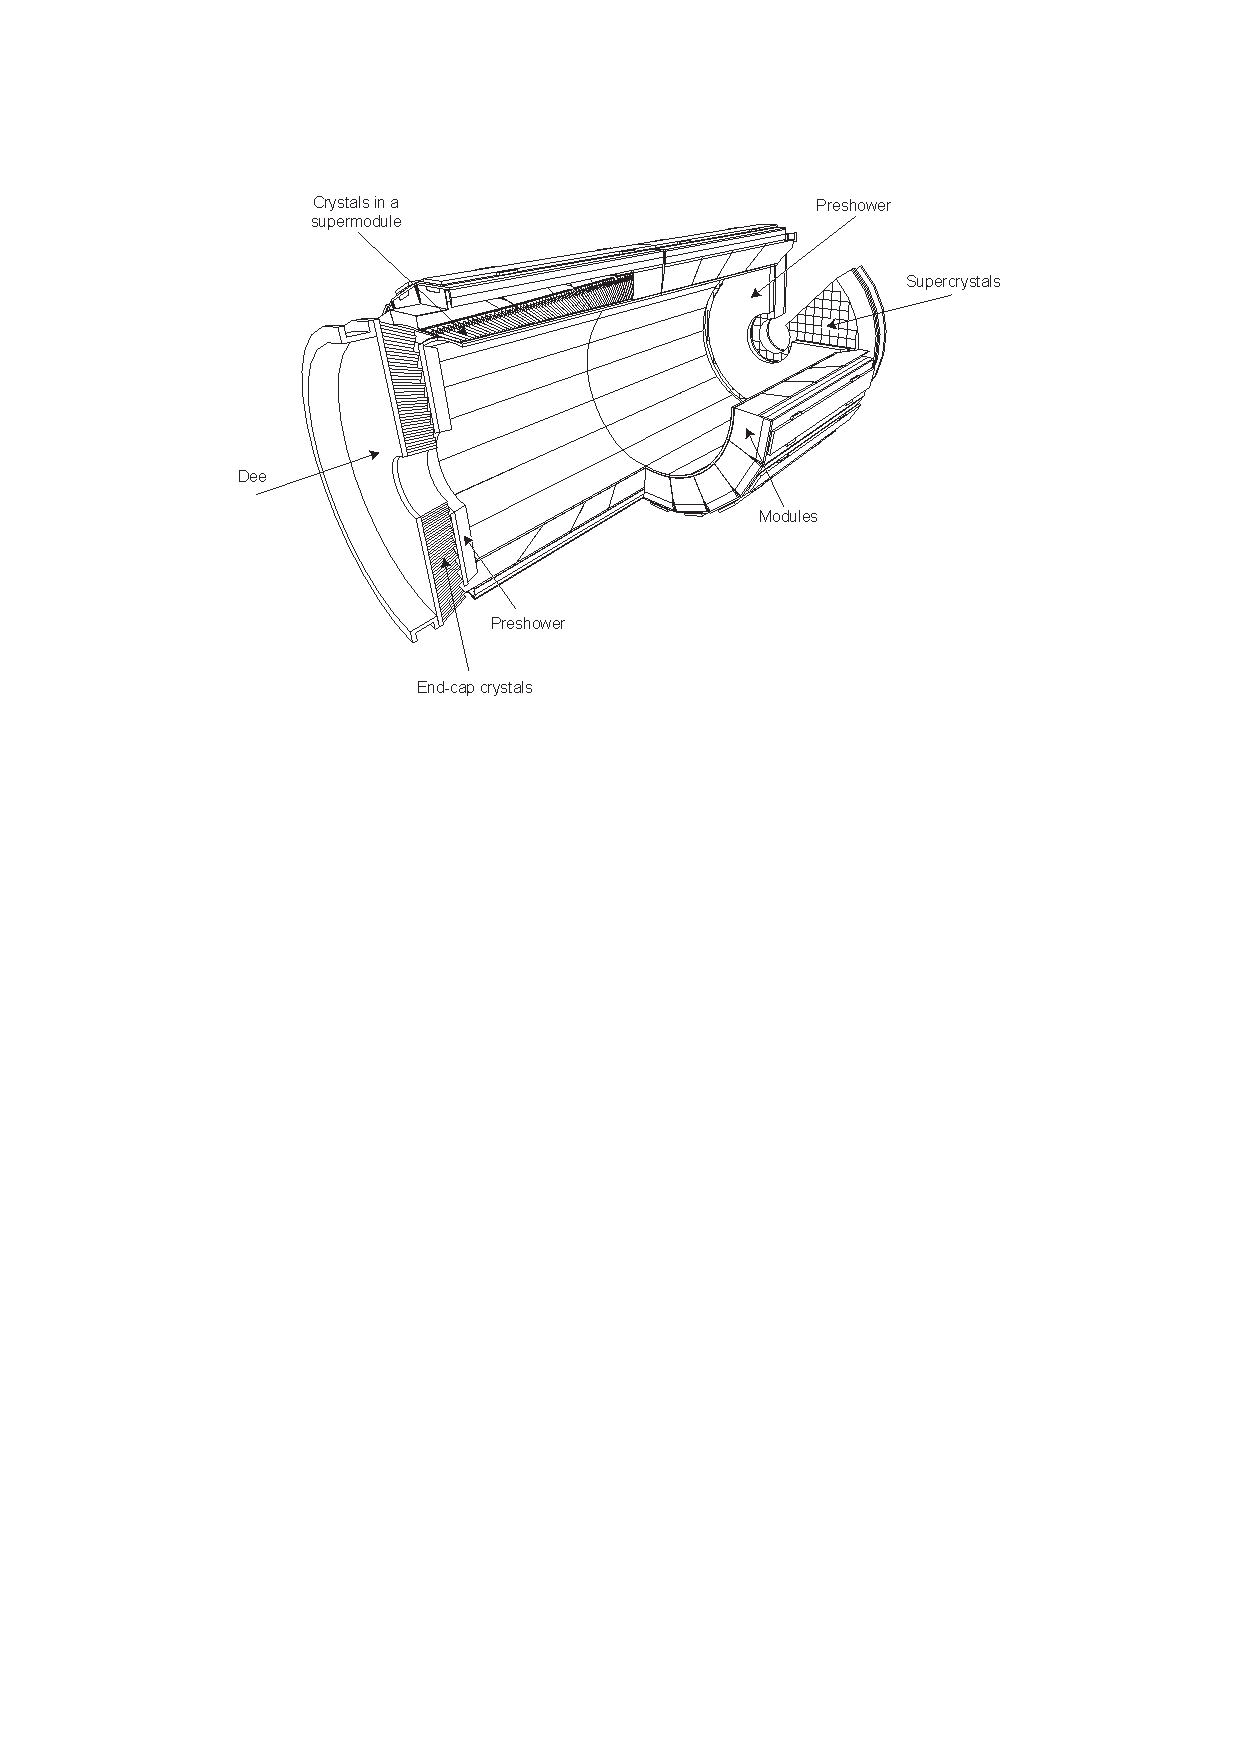
\includegraphics[width=1.5\cmsFigWidth]{figures/cms-ecallayout}
    \caption{Layout of the CMS electromagnetic calorimeter, showing the barrel, endcaps, and preshower~\cite{1748-0221-3-08-S08004}.}
    \label{fig:cms-ecallayout}
  \end{center}
\end{figure}

\begin{figure}[hbtp]
  \begin{center}
    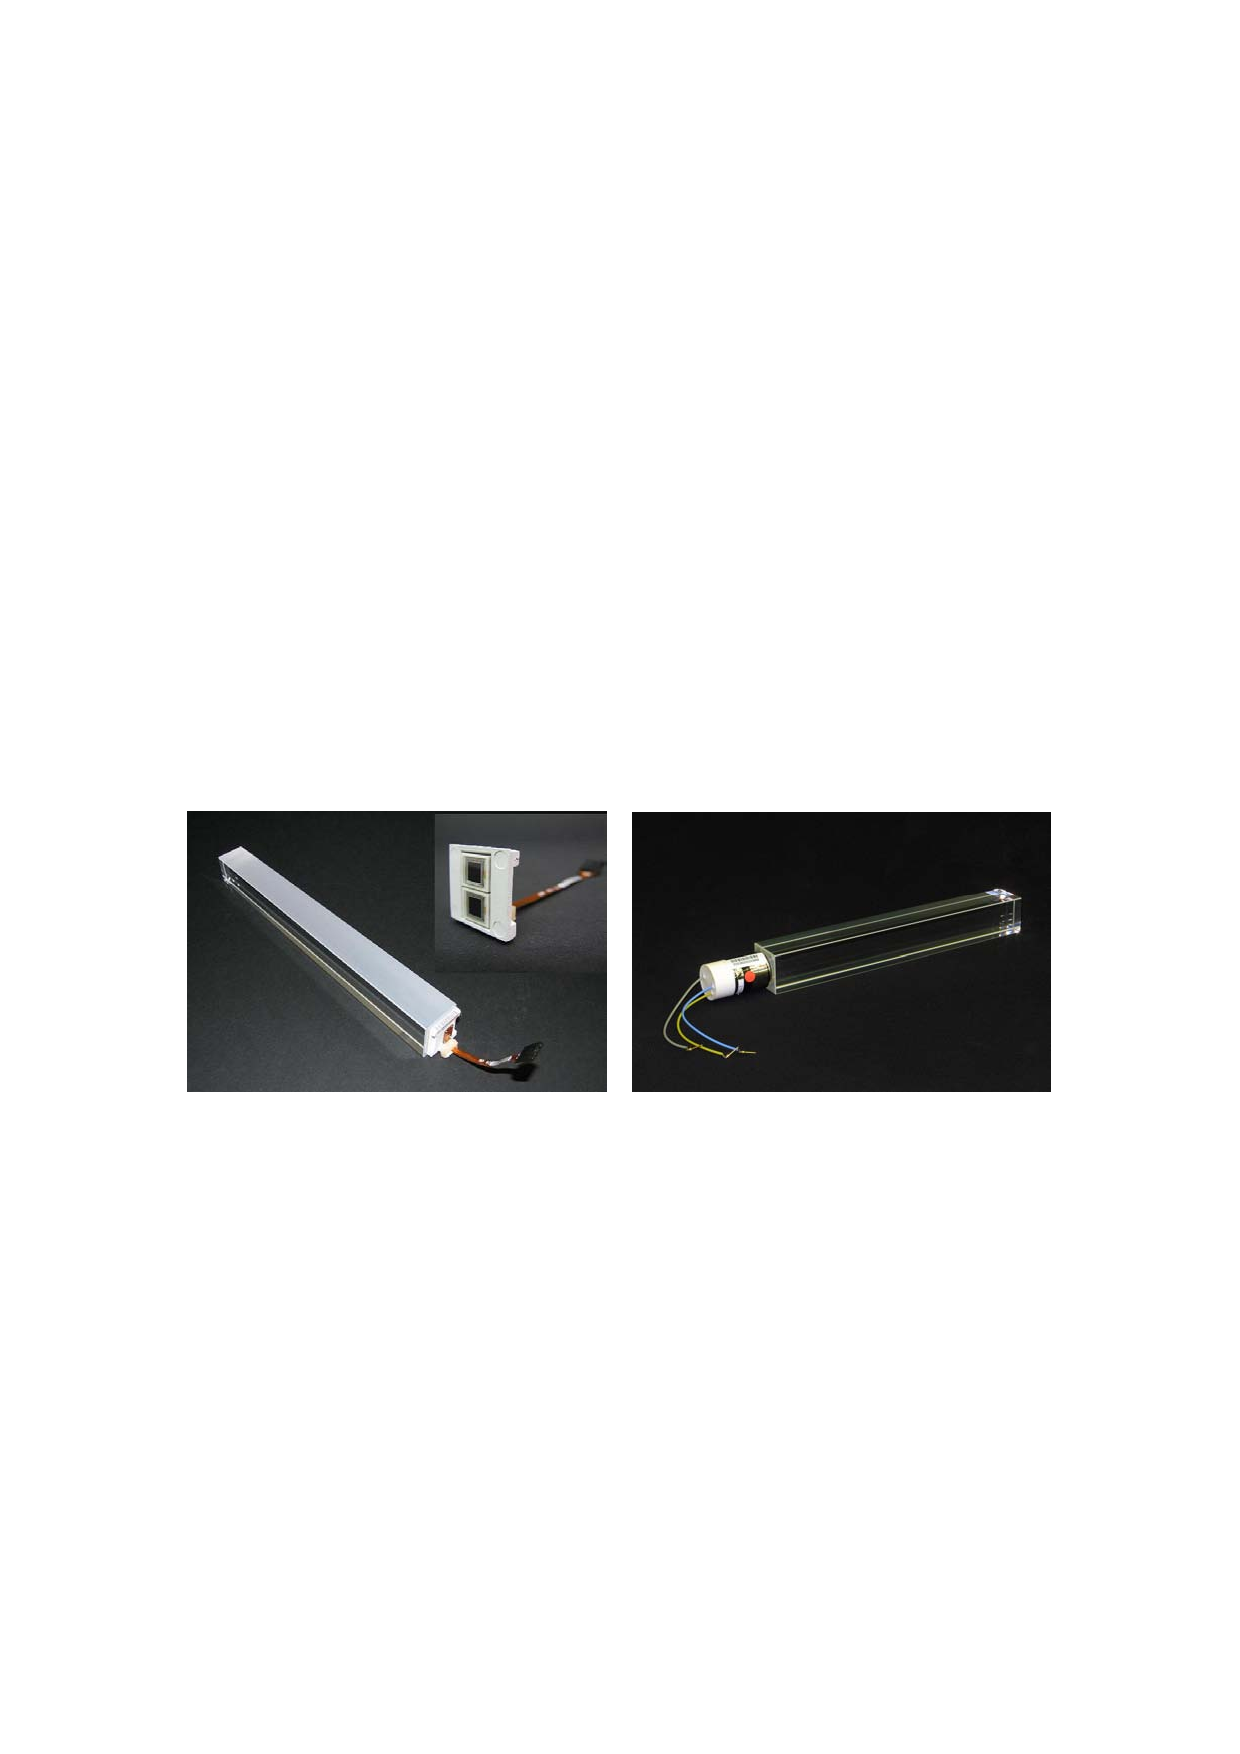
\includegraphics[width=2.5\cmsFigWidth]{figures/cms-ecal-crystals}
    \caption{(\cmsLeft) ECAL barrel crystal with attached APD. (\cmsRight) ECAL endcap crystal with attached VPT.~\cite{1748-0221-3-08-S08004}}
    \label{fig:cms-ecal-crystals}
  \end{center}
\end{figure}

The barrel extends from an inner radius of 1.29 m to an outer radius of 1.77 m. In the barrel, the detector granularity is 360-fold in $\phi$ and 170-fold in $\eta$. The crystals have a truncated pyramidal shape that varies with their position in $\eta$, with a cross-sectional area of approximately 22$\times$22 mm$^2$ at the front face (closest to the beam line) and 26$\times$26 mm$^2$ at the rear face, and a length of 230 mm (corresponding to 25.8 radiation lengths). Groups of 2$\times$5 barrel modules are referred to as sub-modules, encased within a 0.1-mm thick wall consisting of an aluminium layer facing the crystal, followed by two layers of glass fibre-epoxy resin. Submodules are grouped together into larger groups called modules (see an example in Figure~\ref{fig:cms-ecal-super}) containing 400 or 500 crystals, whose shape depends on the position in $\eta$ of the module. Four modules form a supermodule, and 18 supermodules form half a barrel.

On either side of the barrel, the ECAL endcaps cover the pseudorapidity range 1.479 $<$ $\abs{\eta}$ $<$ 3.0. Endcap crystals have a truncated pyramidal shape similar to barrel crystals, with a front face cross-sectional area of about 28.62$\times$28.62 mm$^2$ and a rear face cross-sectional area of 30$\times$30 mm$^2$, and a length of 220 mm (24.7 radiation lengths). They are arranged in groups of 5$\times$5 known as supercrystals, enclosed in a carbon-fibre alveolar wall. Each half of an endcap disk, called a Dee, is composed of 138 full supercrystals and 18 partial supercrystals; Figure~\ref{fig:cms-ecal-super} shows a Dee made up of supercrystals.

\begin{figure}[hbtp]
  \begin{center}
    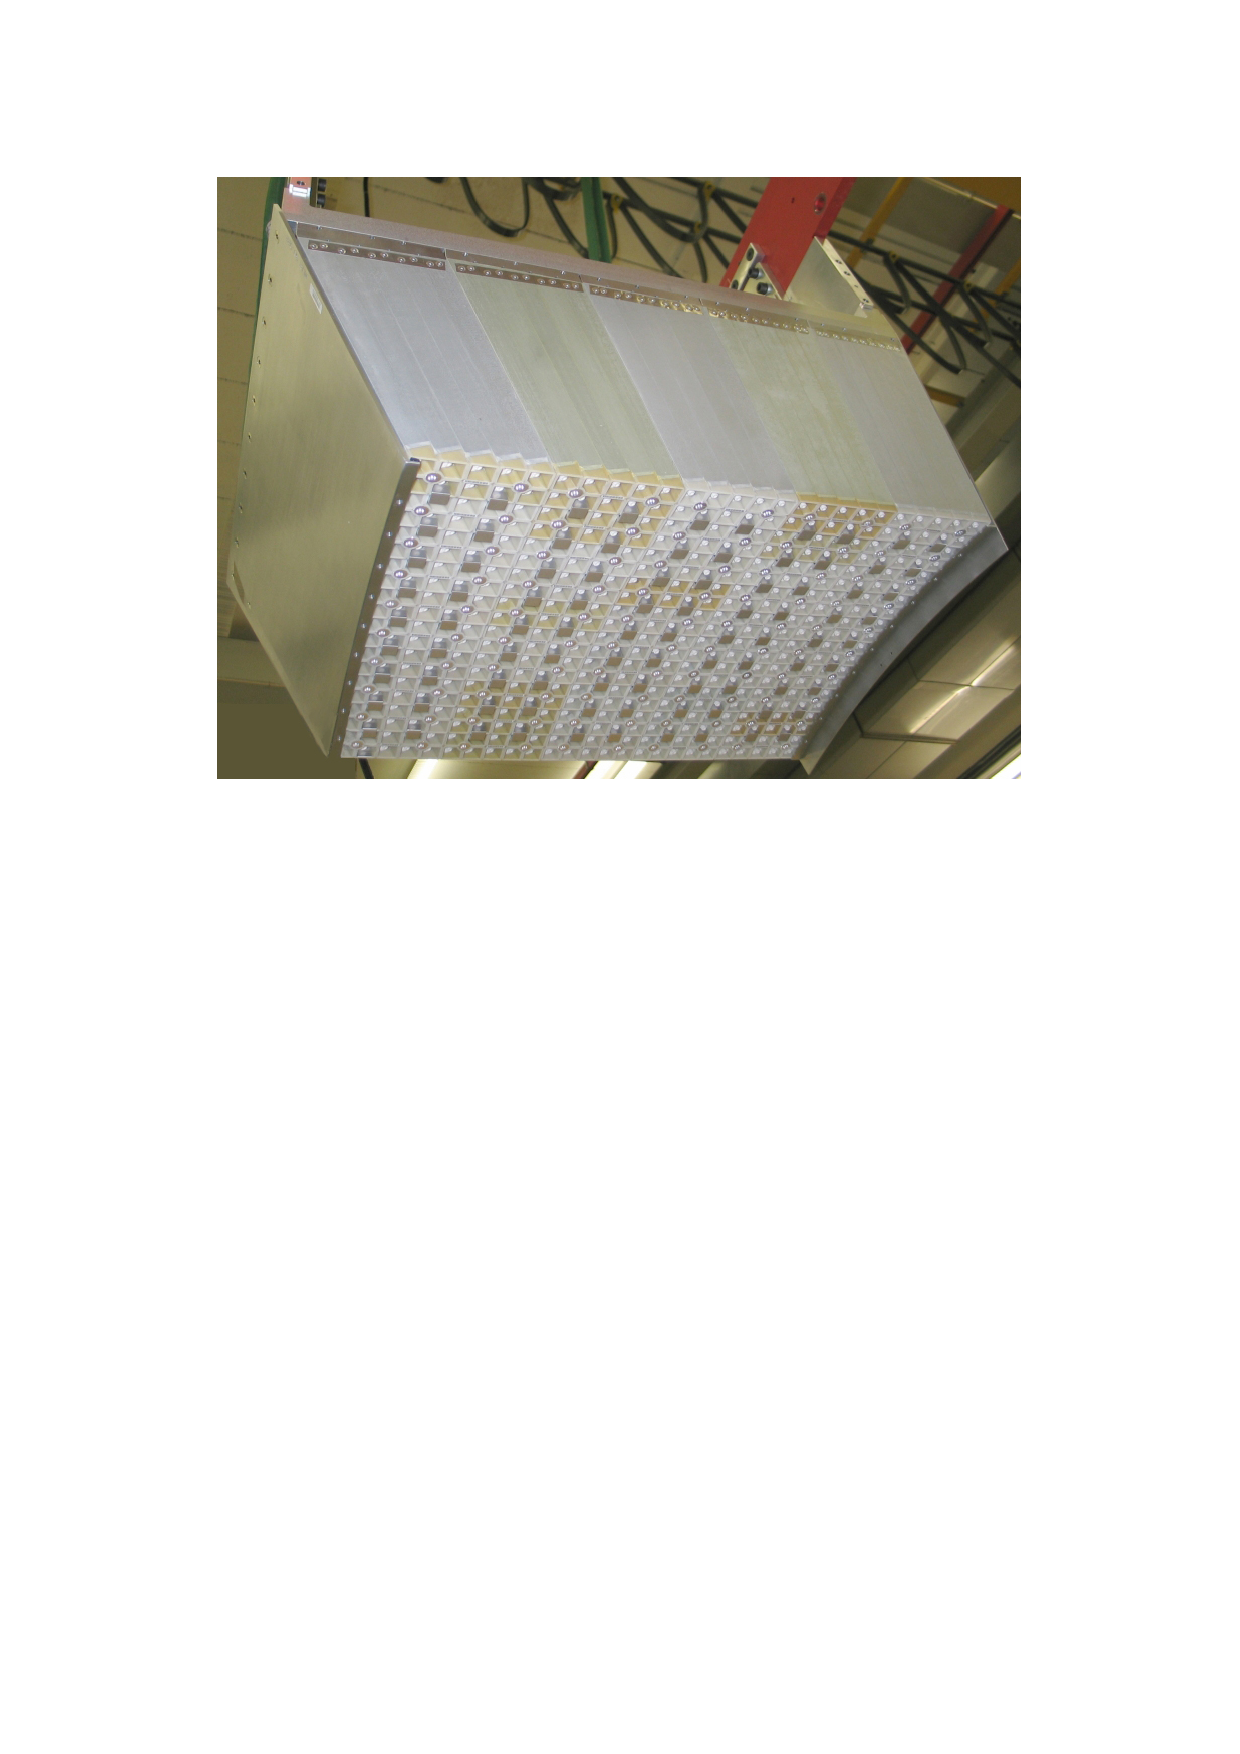
\includegraphics[width=\cmsFigWidth]{figures/cms-ecal-supermodule}
    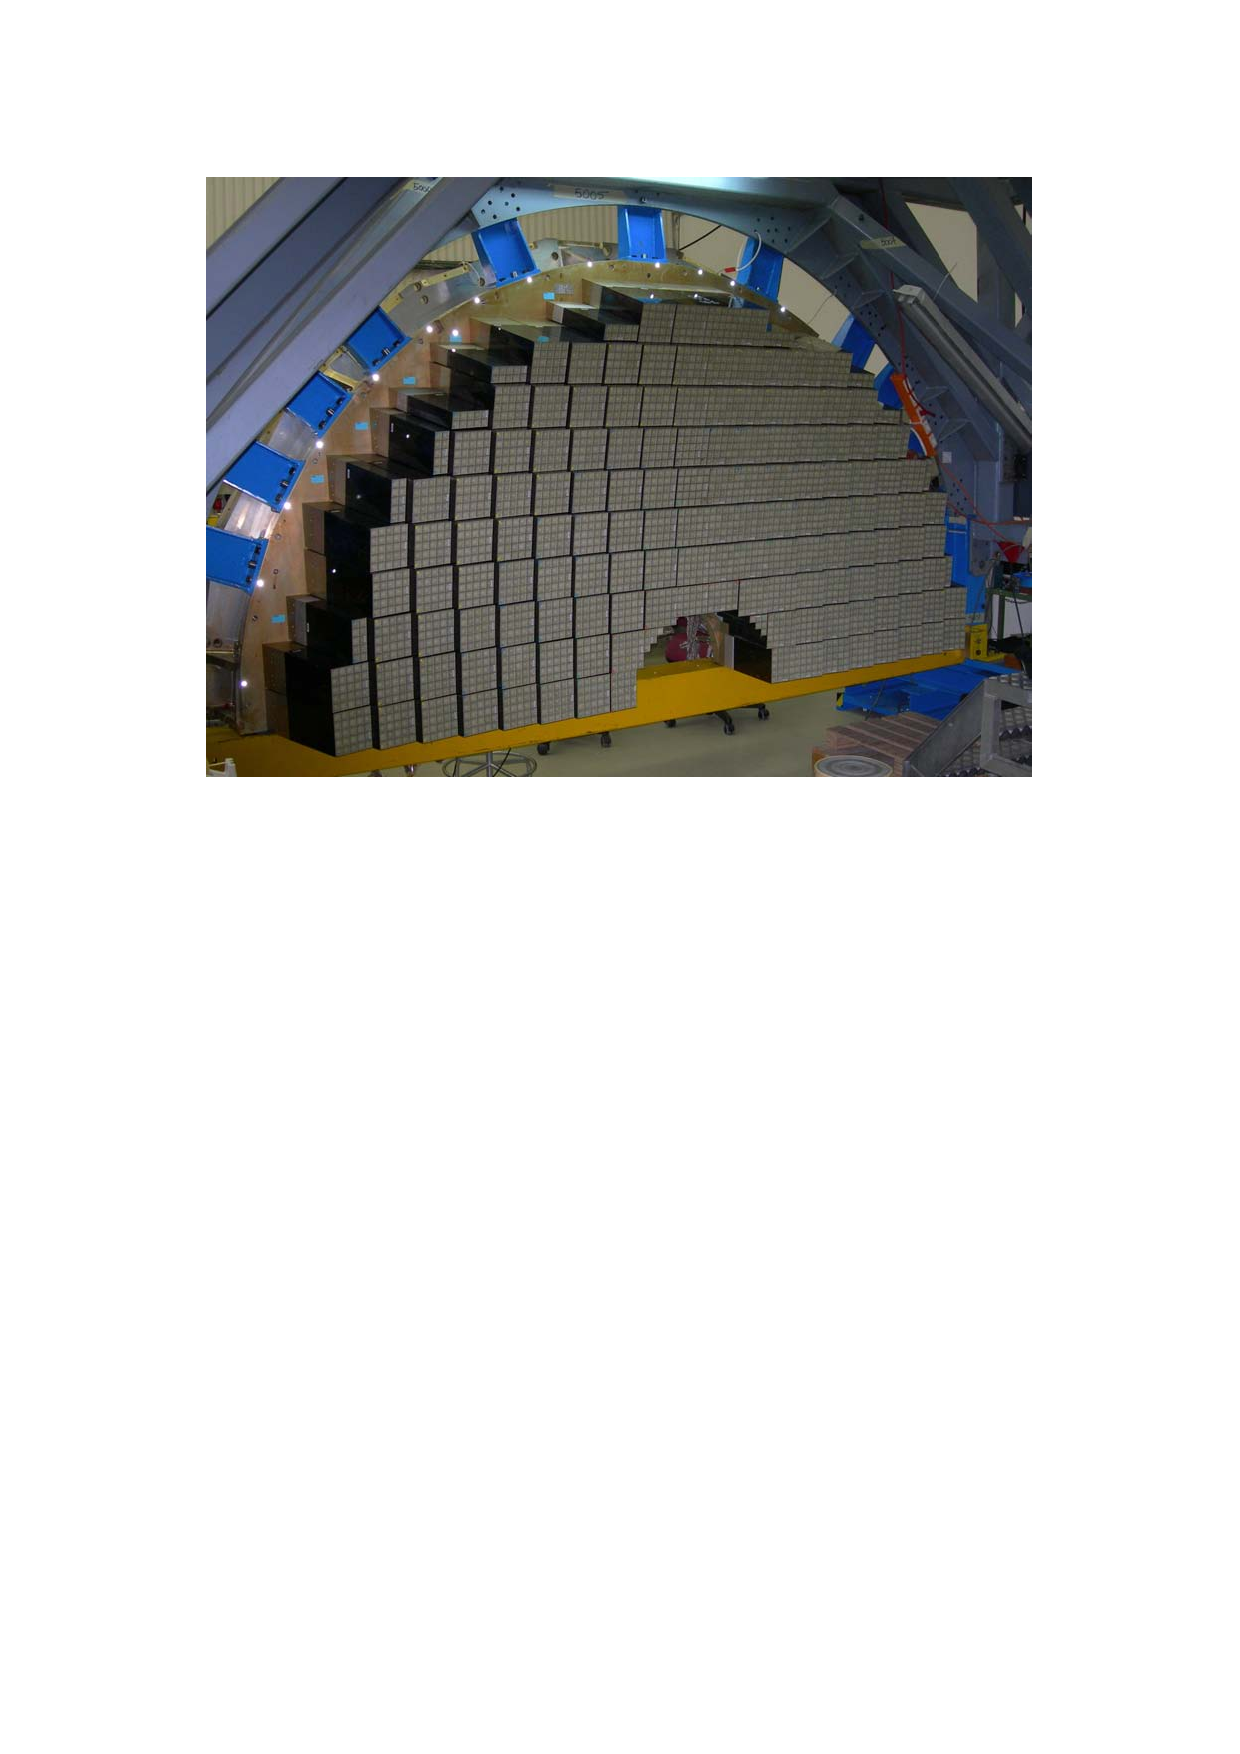
\includegraphics[width=\cmsFigWidth]{figures/cms-ecal-supercrystal}
    \caption{(\cmsLeft) Module from the ECAL barrel. (\cmsRight) Supercrystals mounted on an ECAL endcap Dee.~\cite{1748-0221-3-08-S08004}}
    \label{fig:cms-ecal-super}
  \end{center}
\end{figure}

Sandwiched between the barrel and each endcap disk is a disk-shaped sampling calorimeter with a thickness of 20 cm; these two disks make up the preshower detector. Its main purposes are neutral pion identification and rejection in the fiducial region 1.653 $<$ $\abs{\eta}$ $<$ 2.6, identify electrons against the background of minimum ionizing particles, and improve the position resolution of electrons and photons in the ECAL. The preshower is two layers thick; each layer consists of a layer of lead radiators for initiating electromagnetic showers, followed by a layer of silicon strip sensors for detecting the showers.

To take advantage of total internal reflection for the collection of scintillation light, all the ECAL crystals (Figure~\ref{fig:cms-ecal-crystals}) have been precisely polished during production. The crystals have a truncated pyramidal shape, which tends to cause nonuniform light collection along their length; thus, in the barrel, one crystal face is left unpolished to compensate for this effect. This technique is not used in the endcaps because the endcap crystal faces are nearly parallel to one another, thus resulting in more uniform light collection. The different magnetic field configuration and particle flux in the barrel and endcaps led to different choices of photodetectors for those two systems: avalanche photodiodes (APDs) for the barrel and vacuum phototriodes (VPTs) in the endcaps. At 18$^{\circ}$ C, approximately 4.5 photoelectrons per MeV of deposited energy are collected by both APDs and VPTs. 

As the number of scintillation photons produced by the crystals and the amplification provided by the photodiodes both tend to decrease with increasing temperature, the temperature of the ECAL detector needs to be maintained at a steady operating temperature during its operation. This is done by a cooling system that uses water as a coolant, maintaining the ECAL at a stable temperature of 18$^{\circ}$ C with an uncertainty of $\pm$0.05$^{\circ}$ C.

For electron or photon energies below 500 GeV, the ECAL energy resolution can be estimated as follows:

\begin{equation}
(\frac{\sigma}{E})^2 = (\frac{S}{\sqrt{E}})^2 + (\frac{N}{E})^2 + C^2
\label{eq:ECAL-resolution}
\end{equation}

In this equation, $S$ is the stochastic term, $N$ is the noise term, and $C$ is the constant term. The stochastic term $S$ comes from stochastic fluctuations in electromagnetic shower containment, a photostatistics contribution of 2.1\% coming from the uncertainty on the number of primary photoelectrons produced per MeV of deposited energy, and fluctuations in the energy deposited in the preshower absorber. The term $N$ accounts for noise due to electronics, the signal digitization process, and energy deposited by pileup particles. Finally, the constant term $C$ covers various sources of systematic error including the nonuniformity of light collection due to crystal shape, intercalibration errors, and leakage of energy from the back of the crystal.

\begin{figure}[hbtp]
  \begin{center}
    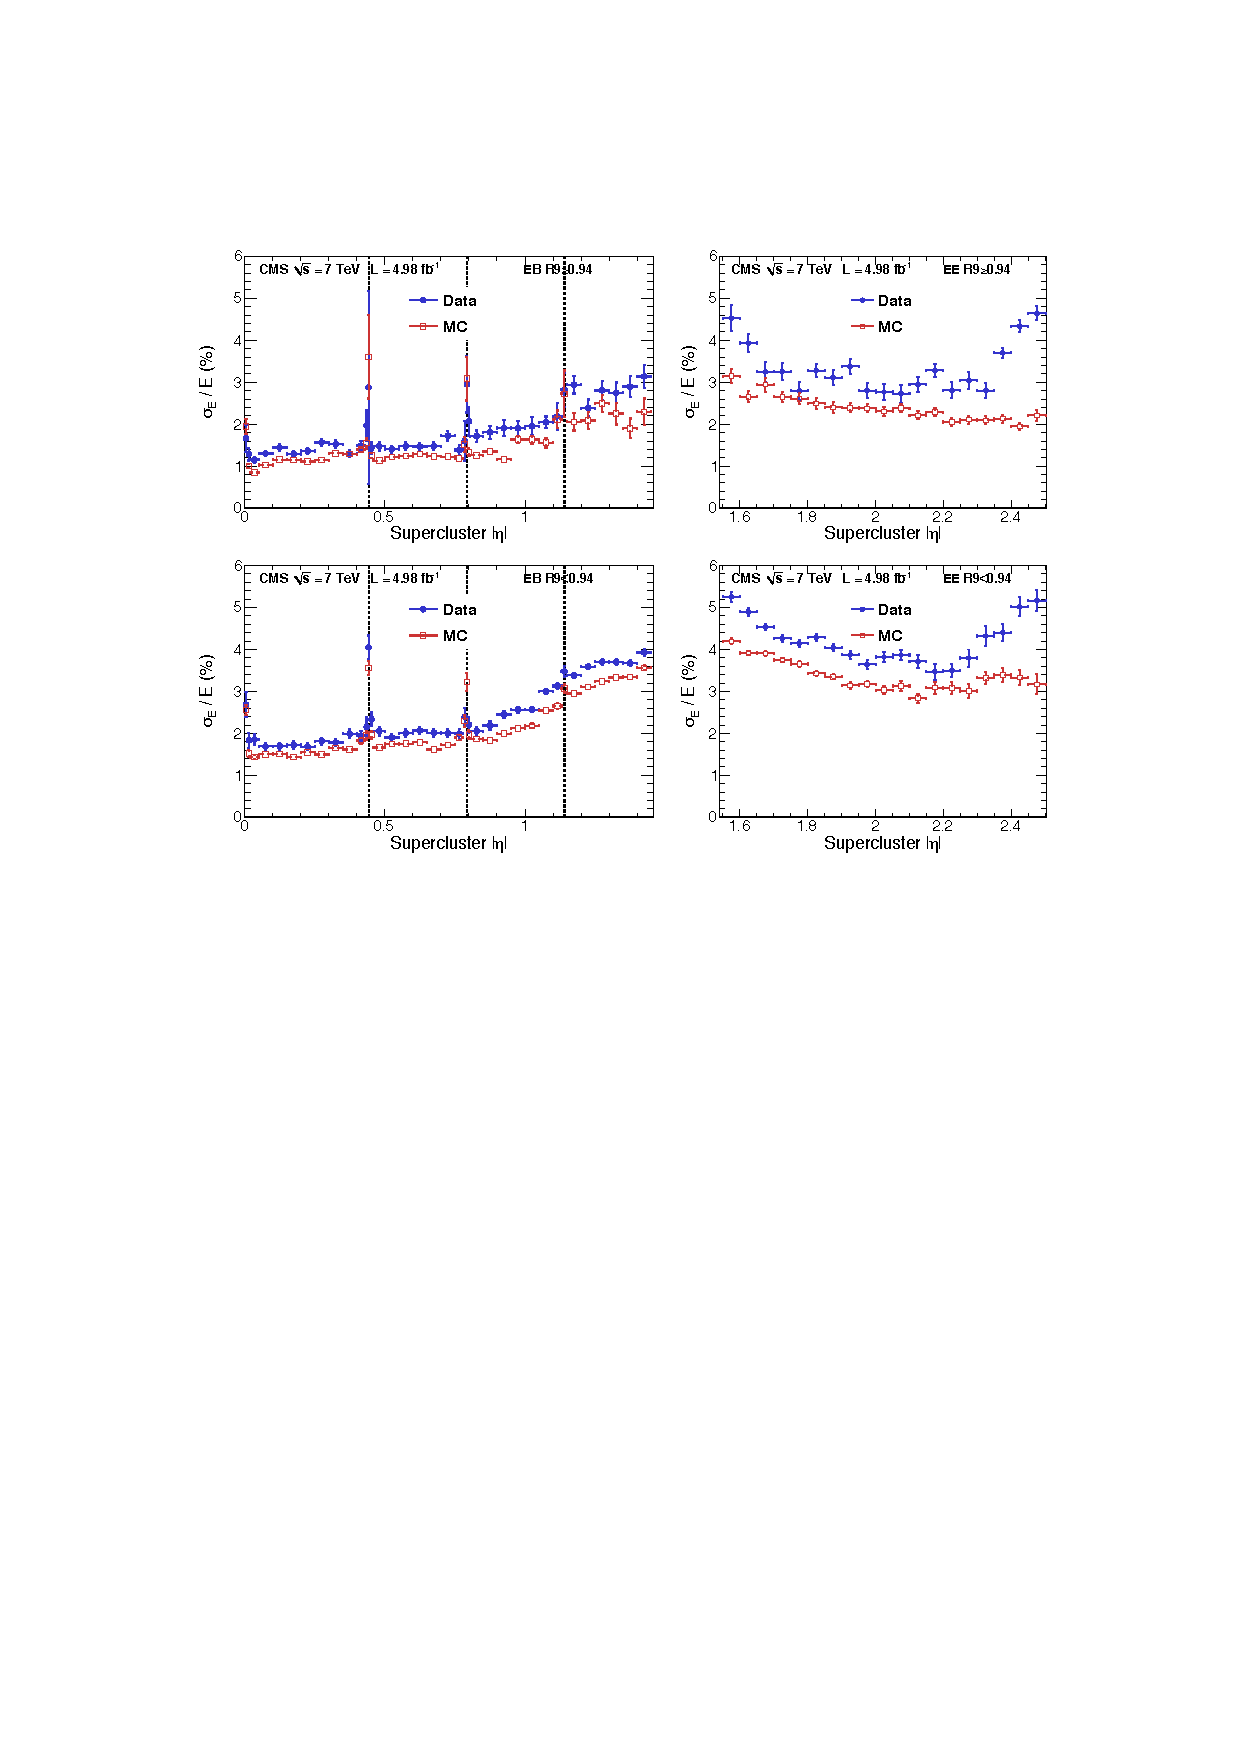
\includegraphics[width=2.0\cmsFigWidth]{figures/cms-ecal-performance}
    \caption{Relative energy resolution in the CMS ECAL detector as a function of supercluster $\abs{\eta}$, measured from $Z\rightarrow$$e^{+}e^{-}$ events~\cite{Chatrchyan:2013dga}. Blue points: data. Red circles: MC events. The term R9 is an ECAL cluster shape parameter used to differentiate between photons that convert in the tracker material (R9$<$0.94) and those that do not (R9$\ge$0.94). (Top \cmsLeft) Barrel, R9$<$0.94. (Top \cmsRight) Endcap, R9$<$0.94. (Bottom \cmsLeft) Barrel, R9$\ge$0.94. (Top \cmsRight) Endcap, R9$\ge$0.94.}
    \label{fig:cms-ecal-performance}
  \end{center}
\end{figure}

Studies done on 7 TeV proton-proton collision events in LHC data and Monte Carlo simulation have measured energy resolutions of less than 2\% for $\abs{\eta} <$ 0.8 in the ECAL barrel, and between 2-5\% everywhere else. These results are shown in Figure~\ref{fig:cms-ecal-performance}.

\subsection{Hadronic calorimeter\label{sec:cms-hcal}}
% HB, HE, HO, HF -- scintillator, absorber, readout

Because proton beams are collided in the LHC and therefore hadronic processes feature in every event, the identification of jets is a crucial part of event selection and reconstruction at CMS. The main goal of the CMS hadronic calorimeter (HCAL) is to measure the energy and direction of hadronic jets. It is also useful for measuring the missing energy in each event, which is needed to identify final states involving not only neutrinos but also possibly exotic particles that do not interact significantly with the detector material, such as neutralinos or dark matter candidates.

The HCAL is a sampling calorimeter extending radially from 1.77 m to 2.95 m from the beam line. Its main goals are to measure the energy deposited by hadronic jets in each event, and to measure indirectly the missing energy in an event. Jet identification is an important part of event selection and reconstruction, and the determination of missing energy is useful not only for final states with neutrinos but also for in the search for final states with exotic particles that can pass through the detector without interaction, such as neutralinos and some dark matter candidates. The HCAL is split up into four subsystems, of which the innermost are the HCAL barrel and endcaps. To provide enough calorimeter material to absorb hadronic showers for jet and missing energy measurement while respecting the spatial constraints from ECAL within and the superconducting solenoid without, the barrel and endcaps are supplemented respectively by the outer calorimeter outside the solenoid and the forward calorimeters outside the muon endcaps. Altogether, these four subsystems provide coverage up to $\abs{\eta} <$ 5.2; their positions are illustrated in Figure~\ref{fig:cms-hcallayout}.

\begin{figure}[hbtp]
  \begin{center}
    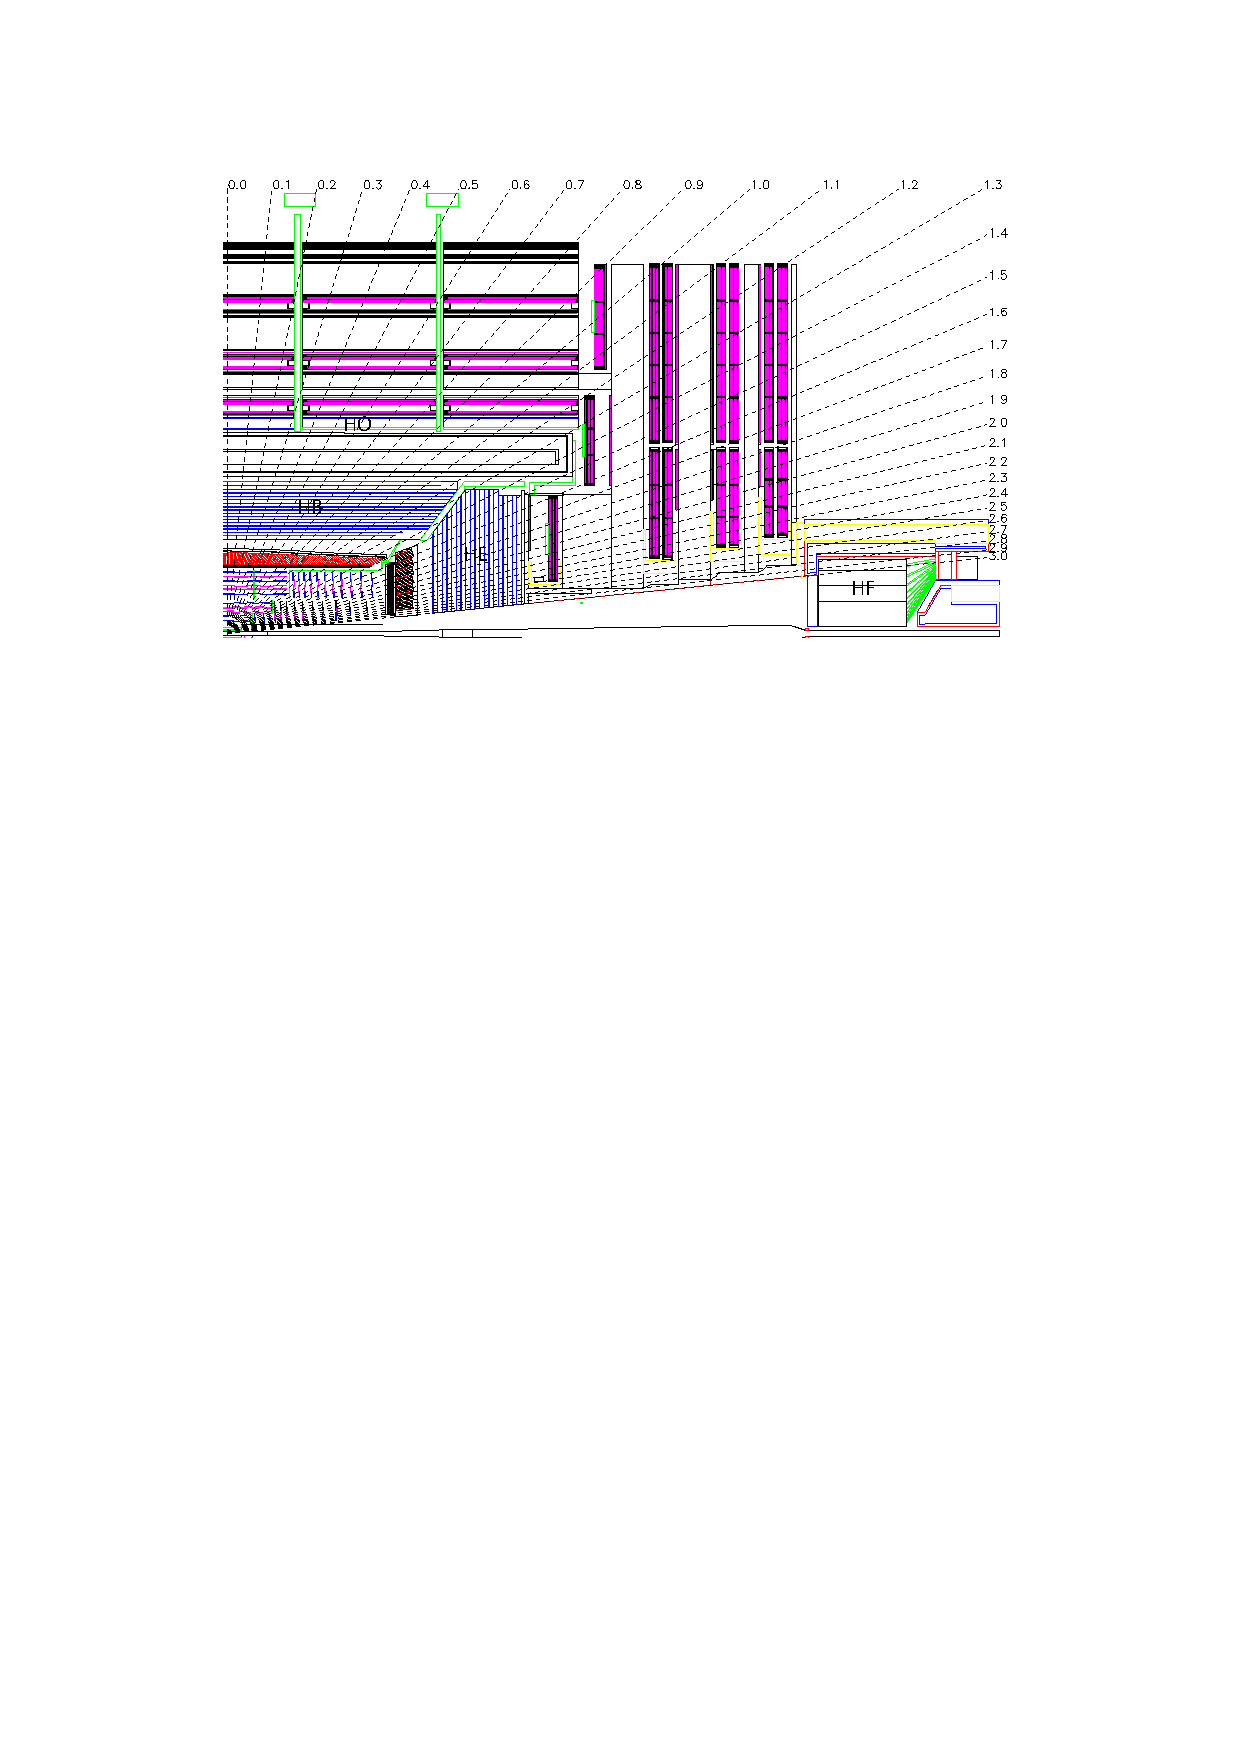
\includegraphics[width=1.75\cmsFigWidth]{figures/cms-hcallayout}
    \caption{Cross-sectional view in the r-z plane of one quadrant of the CMS detector, showing the layout of the CMS hadronic calorimeter and the positions of the HB, HE, HO, and HF~\cite{1748-0221-3-08-S08004}.}
    \label{fig:cms-hcallayout}
  \end{center}
\end{figure}

The barrel system (HB) covers up to $\abs{\eta}$ $<$ 1.3. It is subdivided longitudinally into two half-barrels, each of which consists of 18 identical wedges, making a total of 36 HB wedges. The wedges are subdivided into 4 azimuthal sectors staggered for optimum coverage, and they hold the absorber plates and scintillator material. The HB absorber is made up of an innermost 40-mm-thick steel front plate, eight 50.5-mm-thick brass plates, six 56.5-mm brass plates, and an outermost 75-mm-thick steel back plate. Passing hadrons interact with the nuclei of the absorber, producing hadronic showers of quarks and gluons. The energy in these showers is deposited in and measured by 17 layers of scintillator material that are interspersed between the absorber plates; layers in azimuthal sectors 1 and 4 fit into slots in the edges of a wedge, while layers in azimuthal sectors 2 and 3 fit into slots in the middle of a wedge. Besides the division into 18 sectors in $\phi$, the scintillator material is also split into 16 sectors in $\eta$, resulting in a granularity of (0.087, 0.087) in ($\eta$, $\phi$).

\begin{figure}[hbtp]
  \begin{center}
    %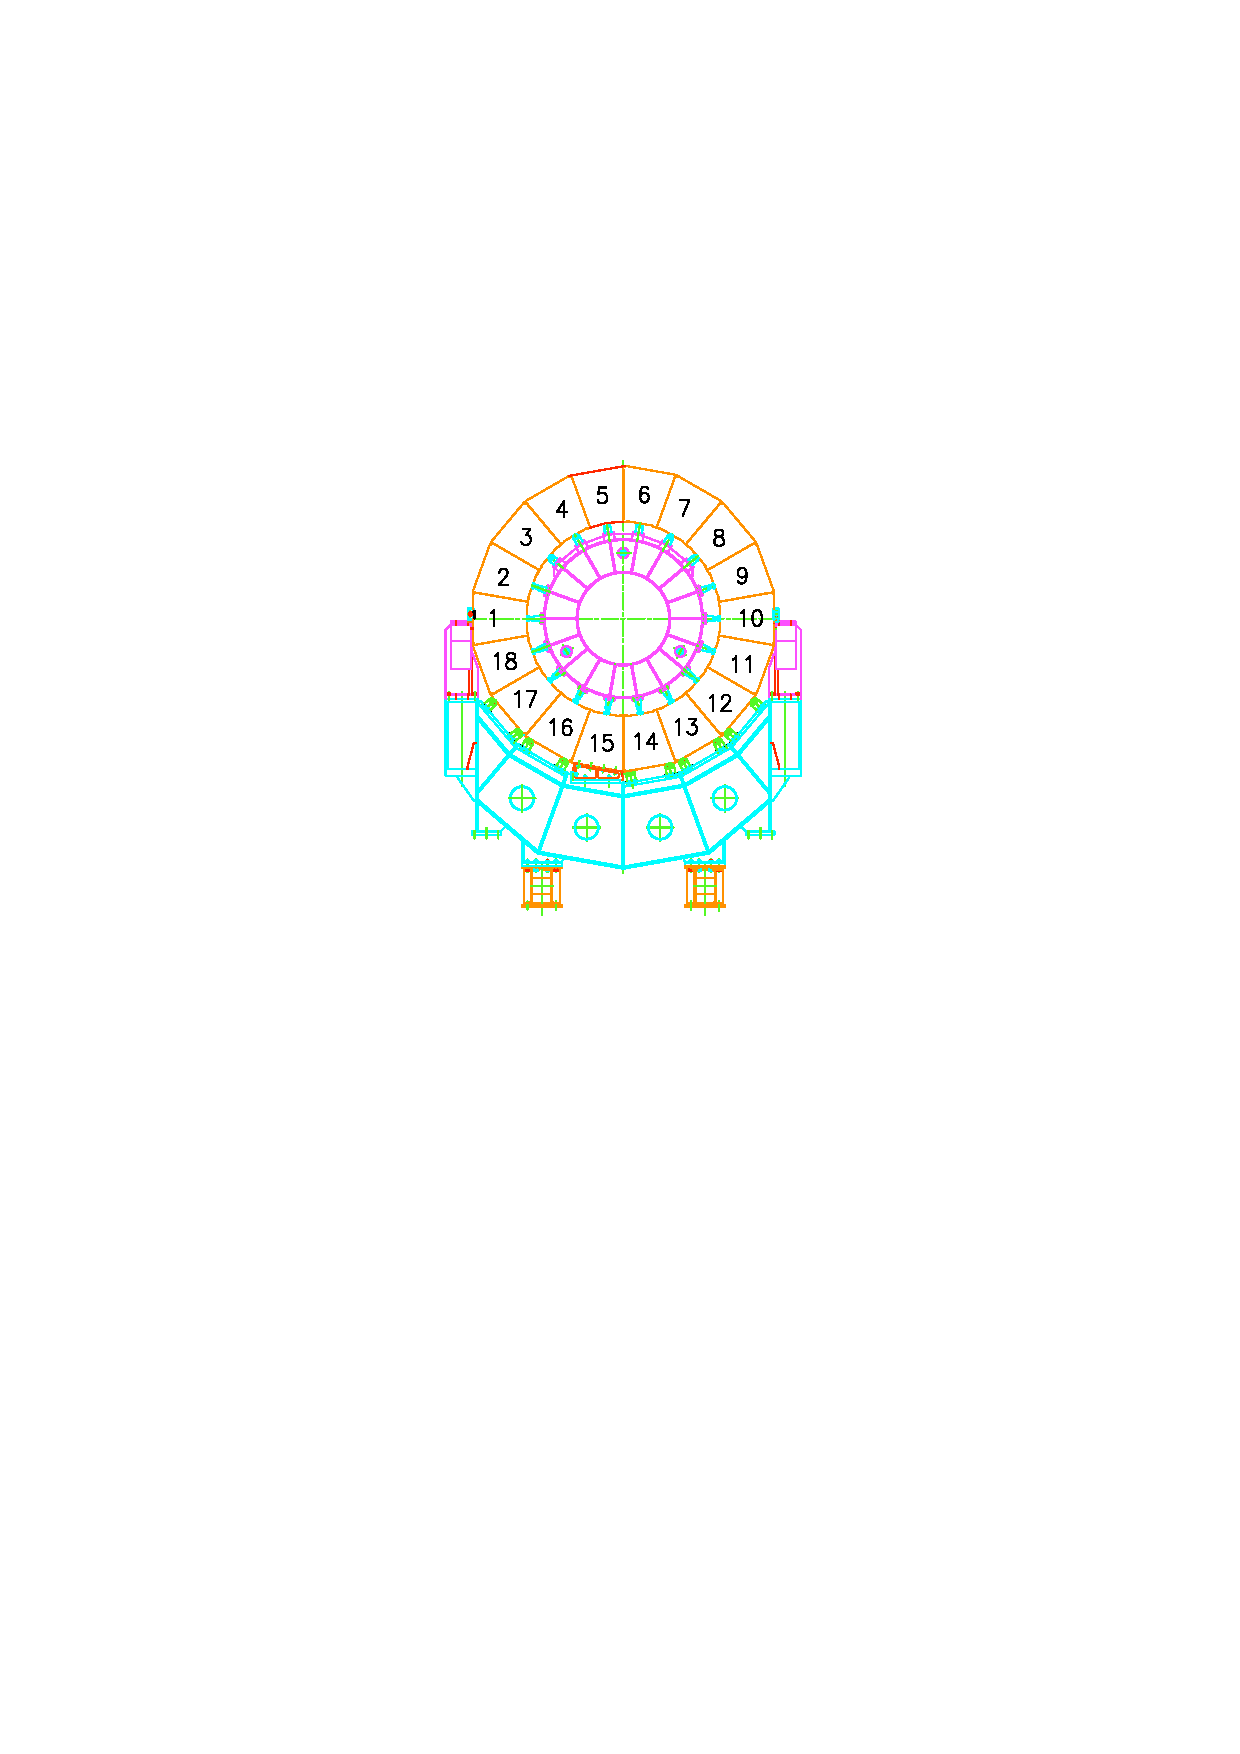
\includegraphics[width=0.9\cmsFigWidth]{figures/cms-hcal-HBnumbering}
    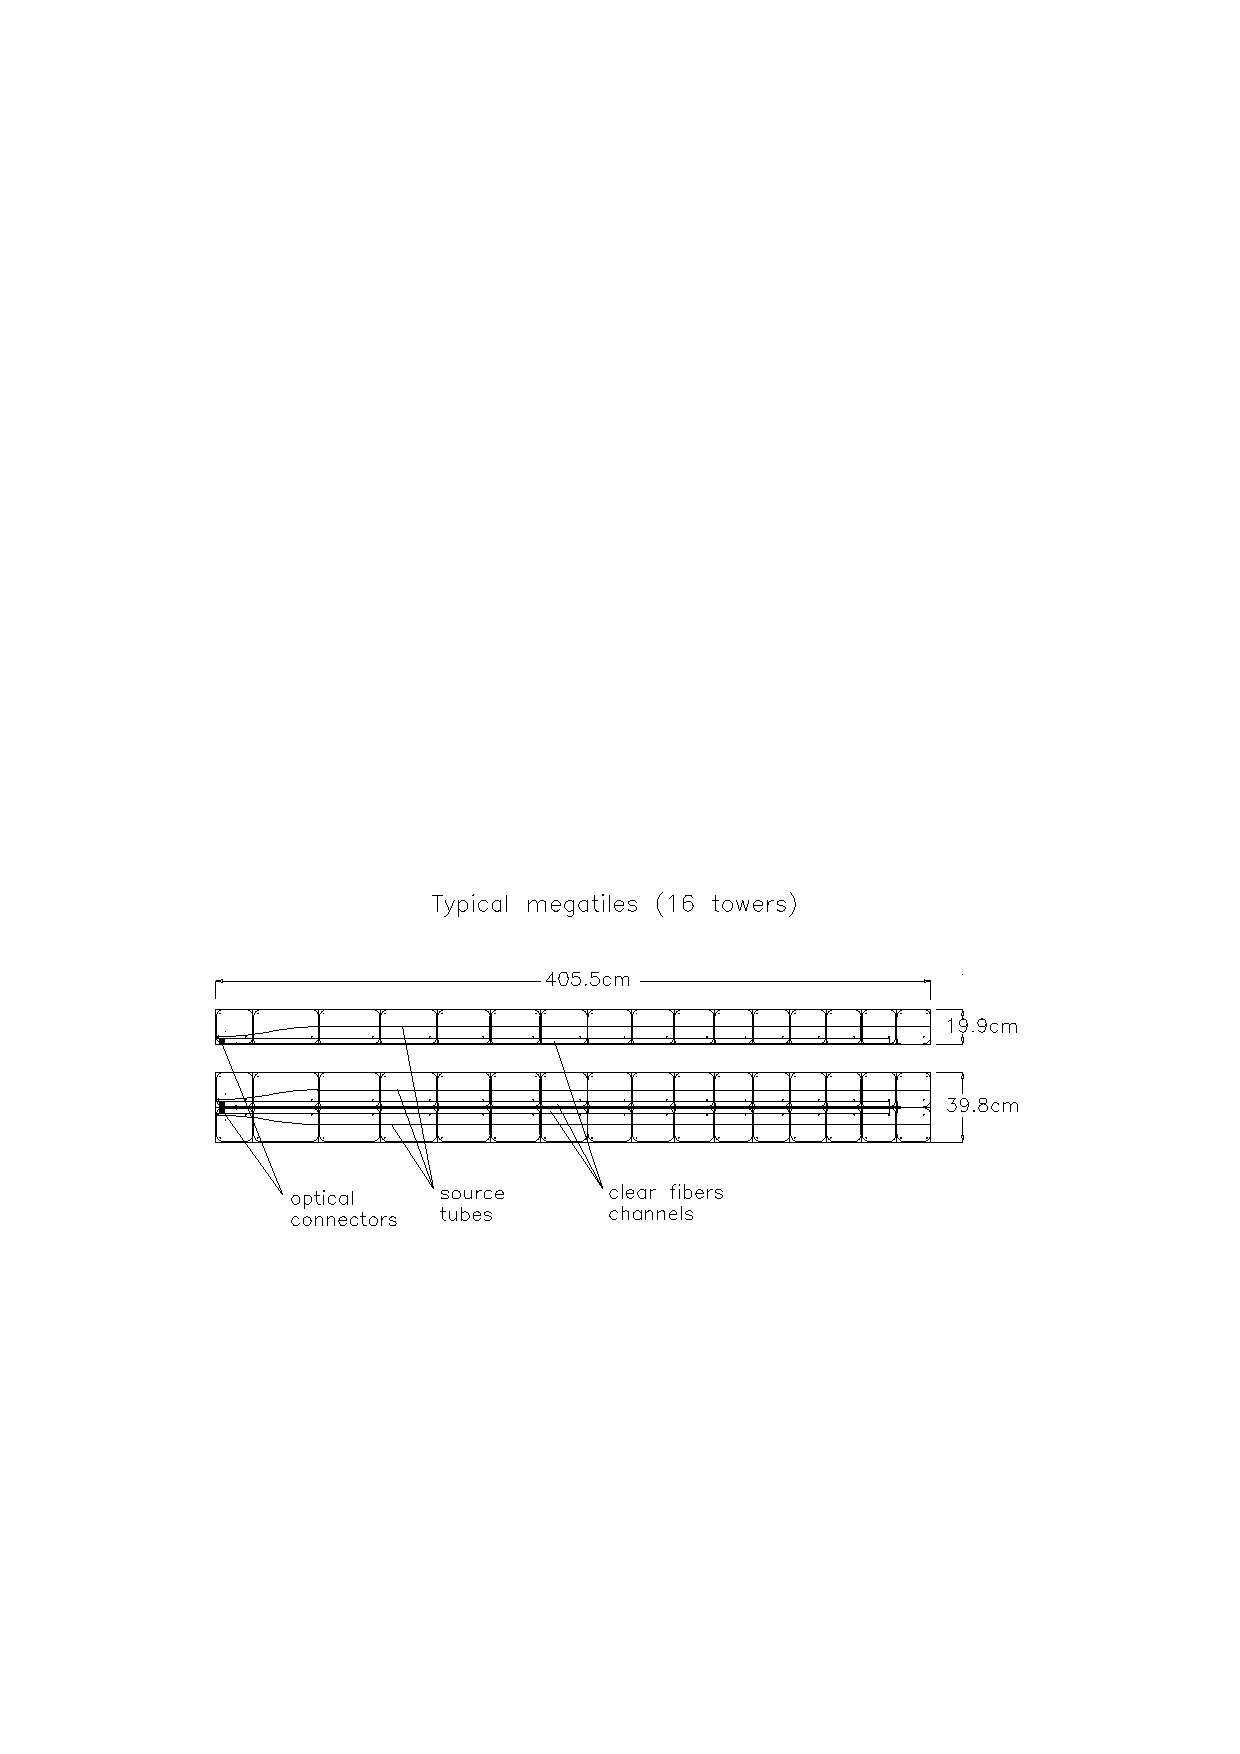
\includegraphics[width=\cmsFigWidth]{figures/cms-hcal-HBtray}
    %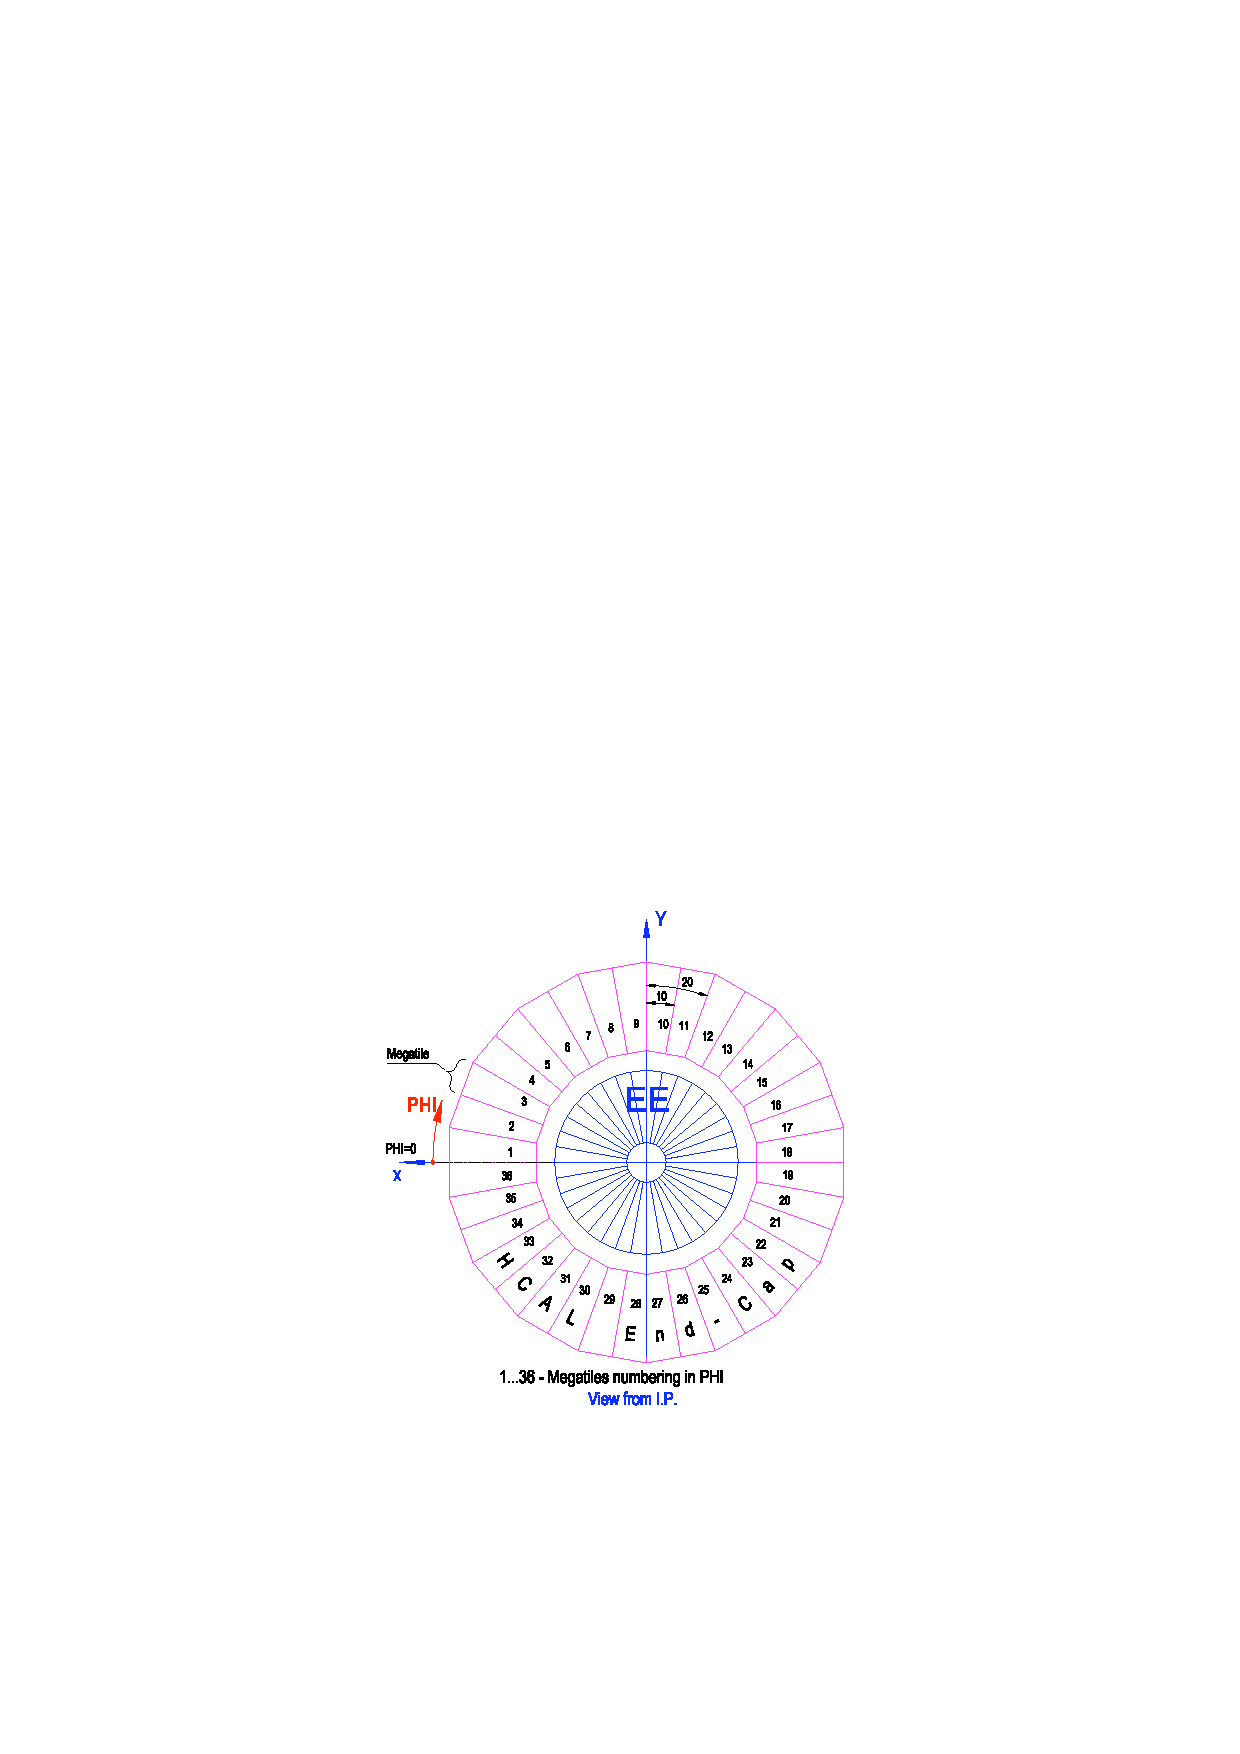
\includegraphics[width=0.9\cmsFigWidth]{figures/cms-hcal-HEnumbering}
    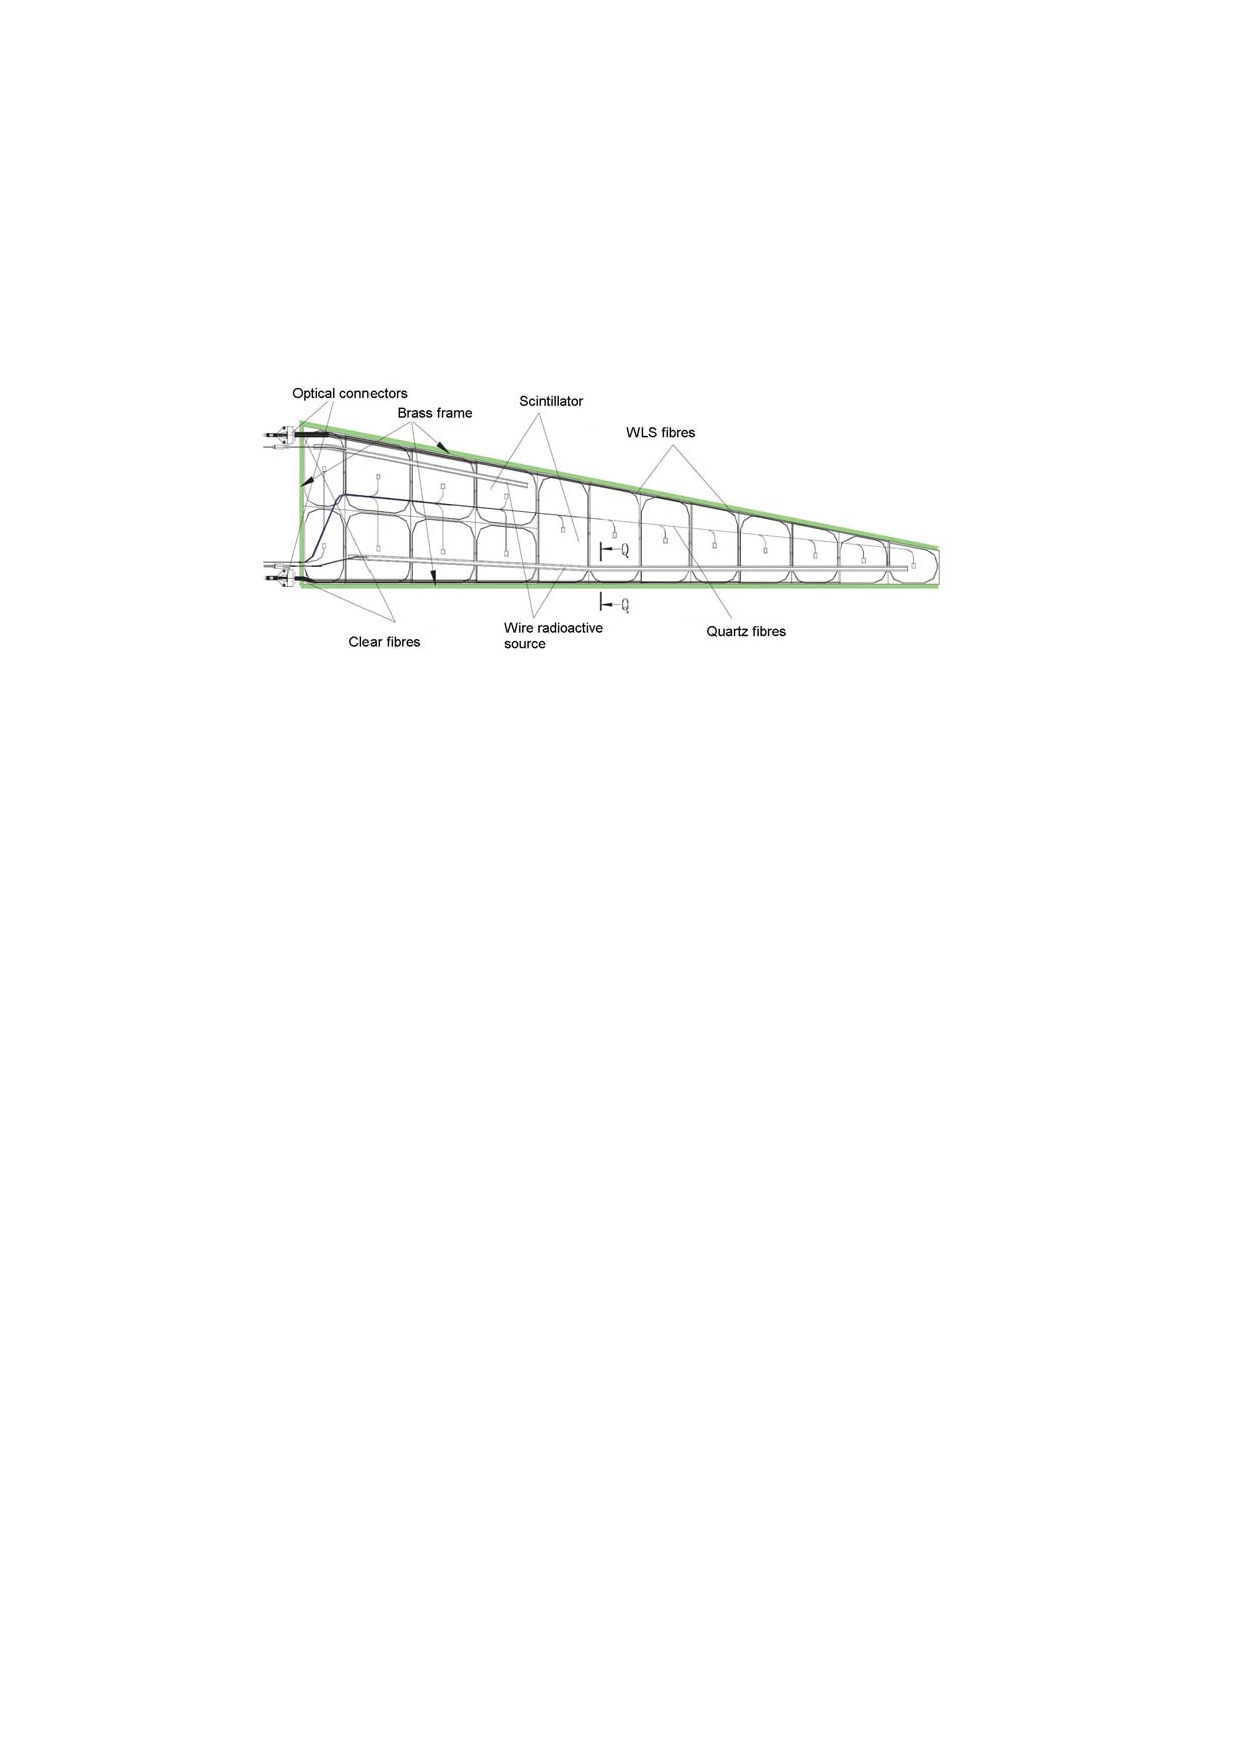
\includegraphics[width=\cmsFigWidth]{figures/cms-hcal-HEtray}
    \caption{(\cmsLeft) HB scintillator tray. (\cmsRight) HE scintillator tray.~\cite{1748-0221-3-08-S08004}.}
    \label{fig:cms-hcal-numbertray}
  \end{center}
\end{figure}

The smallest scintillator unit is called a tile; tiles in layer 0 are made of Bicron BC408 and primarily serve to sample hadronic showers that develop between the HB and the ECAL barrel, while tiles in layers 1-16 are made of of Kuraray SCSN81 plastic scintillator. Tiles in a given azimuthal layer are grouped into units called trays for ease of assembly, access, and individual testing; each barrel layer contains a total of 108 trays. The scintillation light produced in each tile is collected by a Kuraray Y-11 wavelength-shifting (WLS) fibre. Each WLS fibre is spliced to a clear Kuraray double-clad fibre that serves all the tiles in the tray and delivers the collected light to an optical decoding unit, which arranges the clear fibres into readout towers and transmits their signals to a hybrid photodiode (HPD) for amplification and readout. Multipixel HPD's were chosen because of the wider range of wavelengths that they can detect and their low sensitivity to magnetic fields; those used in the HB, HE, and HO have a gain of roughly 2000.

The endcap system (HE) disks on either side of the HB are mounted onto the iron yoke of the muon endcap system and span the pseudorapidity range 1.3 $<$ $\abs{\eta}$ $<$ 3. The disks are subdivided azimuthally into 36 identical wedges and 18 layers, with 79-mm-thick brass absorber plates. The HE contains a total of 20916 trapezoidal scintillator tiles, arranged into 1368 trays, with a granularity of (0.087, 0.087) in ($\eta$, $\phi$) for $\abs{\eta} <$ 1.6 and (0.087, 0.087) for $\abs{\eta}$ $\geq$ 1.6. The collection of scintillation light by WLS fibres and the transmission of the collected signal from tray to HPD for readout is similar to the design of the HB. Figure~\ref{fig:cms-hcal-numbertray} shows schematic diagrams of both HB and HE trays.

The cylindrical outer calorimeter (HO) is located outside the solenoid, taking advantage of the solenoid coil as an additional sampling layer for late-starting hadronic showers. The thickness in hadronic interaction lengths $\lambda_I$ of the HE + HB ensembles varies with $\eta$ between 7-11 $\lambda_I$; when the HO is considered, the total thickness varies from 10-15 $\lambda_I$. The HO layers are mounted within the iron yoke that returns the magnetic field of the solenoid; they are the first sensitive layer in each of the 5 rings of the yoke. Each layer of the HO is divided into 12 sectors in $\phi$, each separated by the dead space of 75-mm-thick steel beams that are part of the support structure of the return yoke and the muon system. The HO layers are 40 mm thick, of which 16 mm corresponds to the detector layer and the rest is occupied by aluminium support structures. The tiles in the HO (see Figure~\ref{fig:cms-hcal-HOtray}) are grouped into towers with a granularity of (0.087, 0.087) in ($\eta$, $\phi$) and have a similar WLS scintillation light collection and HPD readout to the HE and HB trays. Each HO tray spans 5$^{\circ}$ in $\phi$ and the entire range of a muon ring in $\eta$. Studies done to assess the effect of the HO on pion energy measurement by the HCAL have shown that the inclusion of energy measurements in the HO significantly recovers the effects of hadronic shower energy leakage and improves energy resolution (see Figure~\ref{fig:cms-hcal-performance}), which also directly improves the accuracy of missing transverse energy (MET) measurement in an event.

\begin{figure}[hbtp]
  \begin{center}
    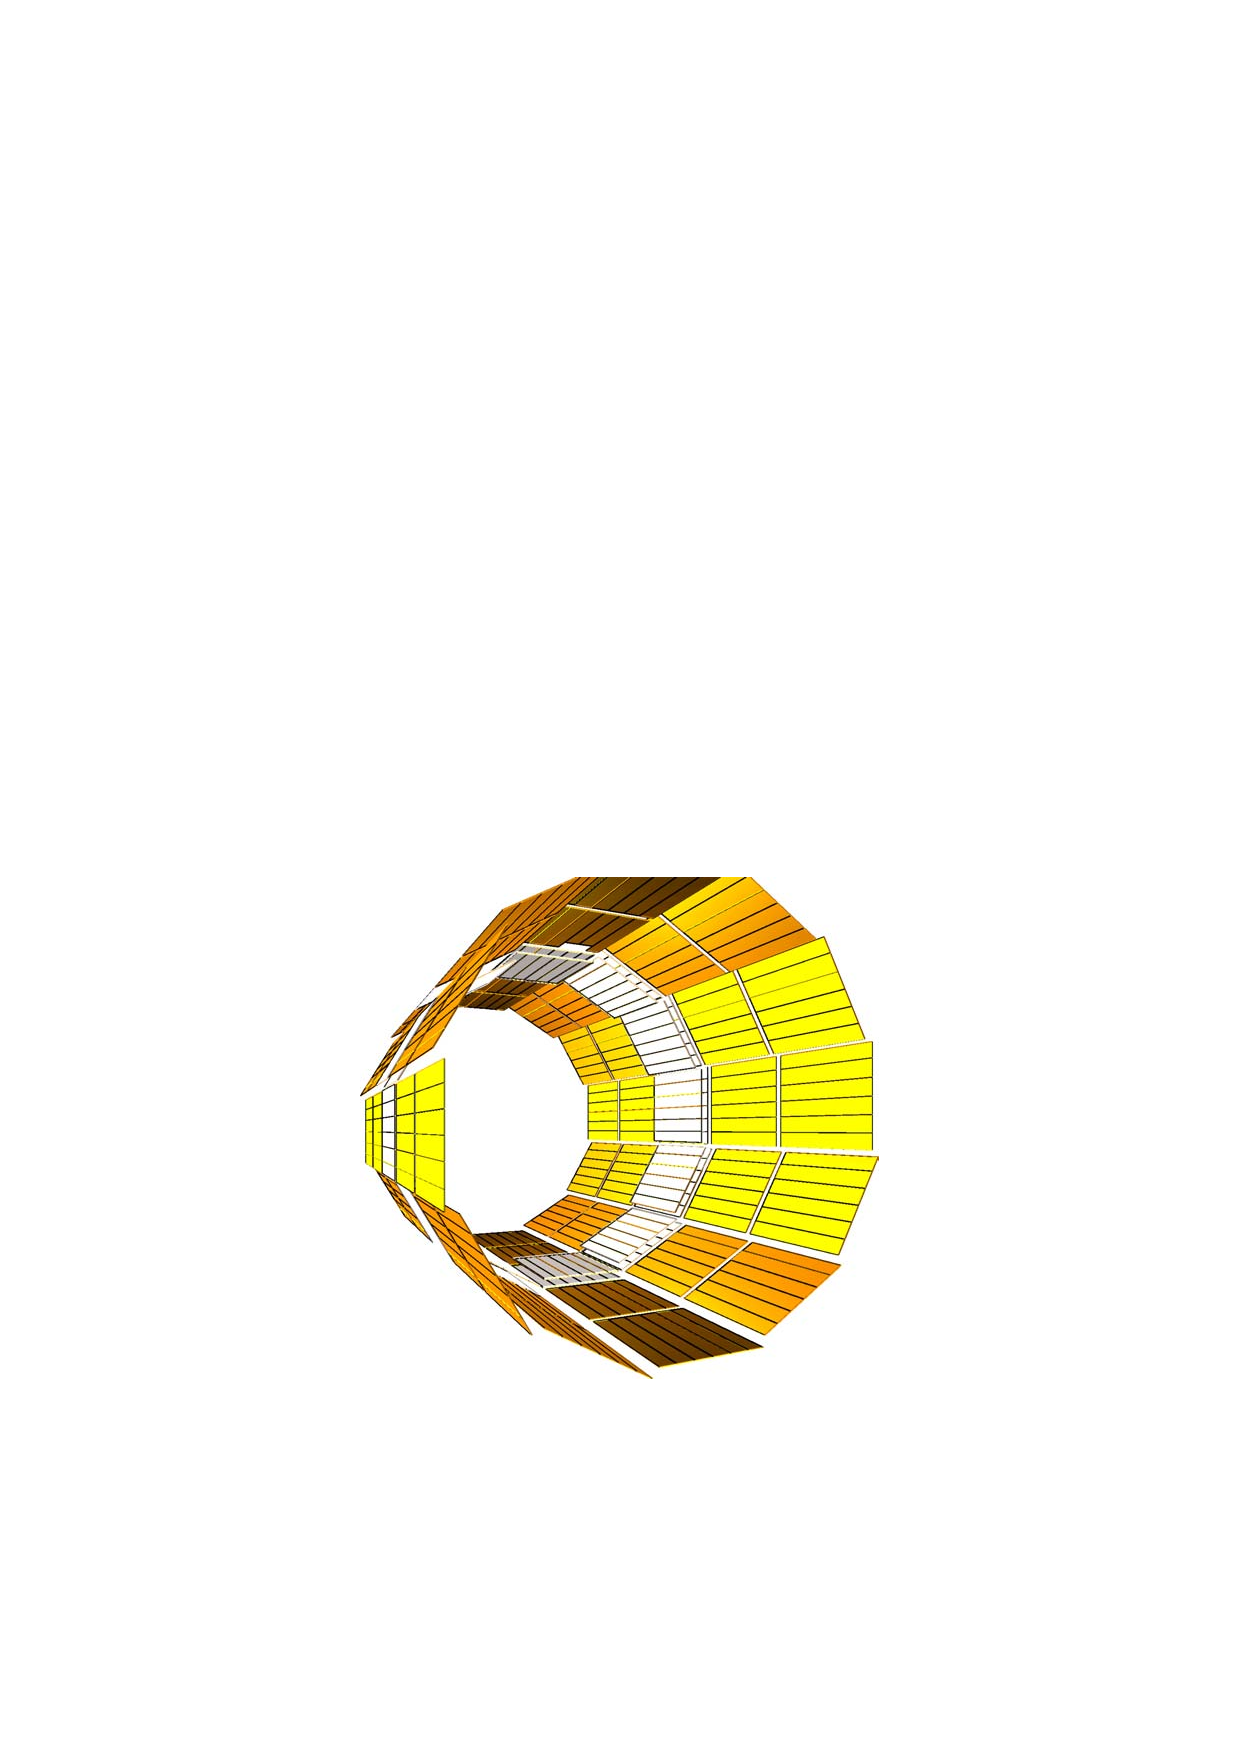
\includegraphics[width=\cmsFigWidth]{figures/cms-hcal-HOtray}
    
\includegraphics[width=\cmsFigWidth]{figures/cms-hcal-HOtile}
    \caption{(\cmsLeft) Positions of all the HO trays. (\cmsRight) Photo of a typical HO tile.~\cite{1748-0221-3-08-S08004}}
    \label{fig:cms-hcal-HOtray}
  \end{center}
\end{figure}

\begin{figure}[hbtp]
  \begin{center}
    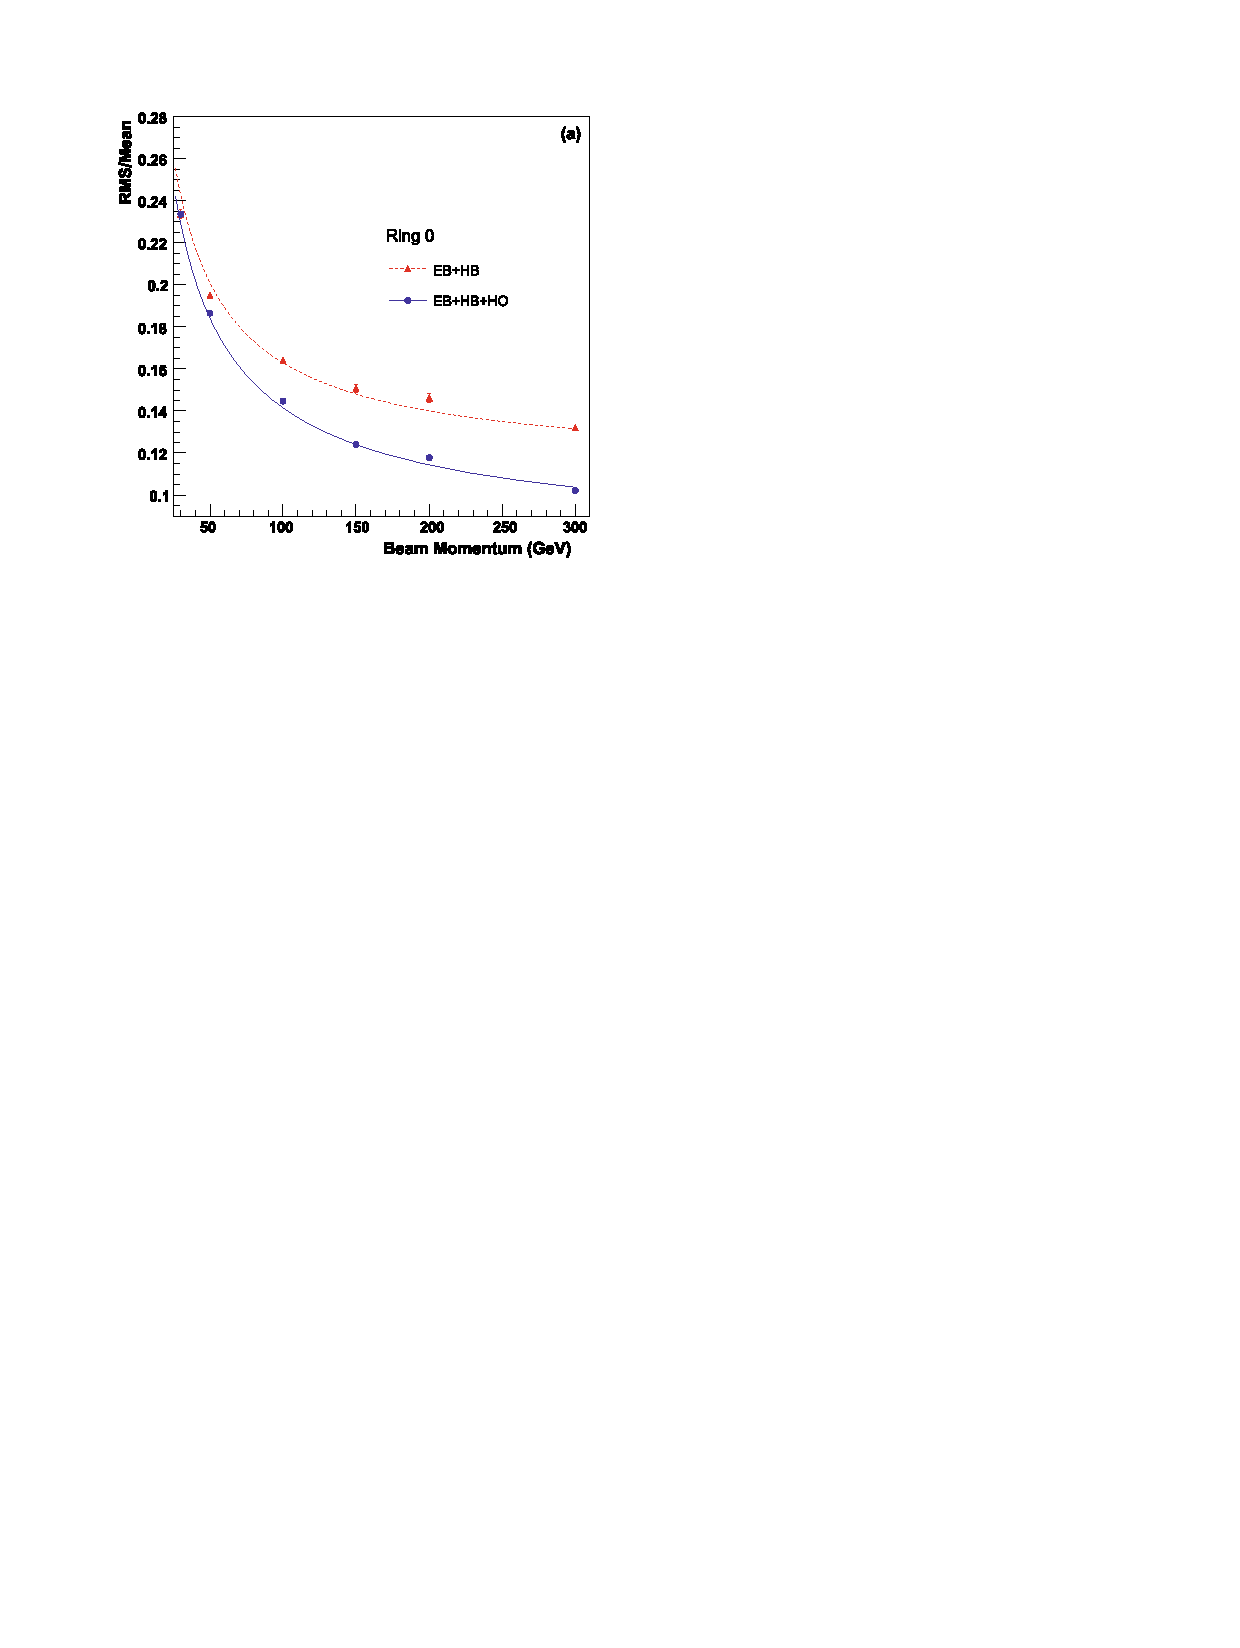
\includegraphics[width=1.2\cmsFigWidth]{figures/cms-hcal-performance1}
    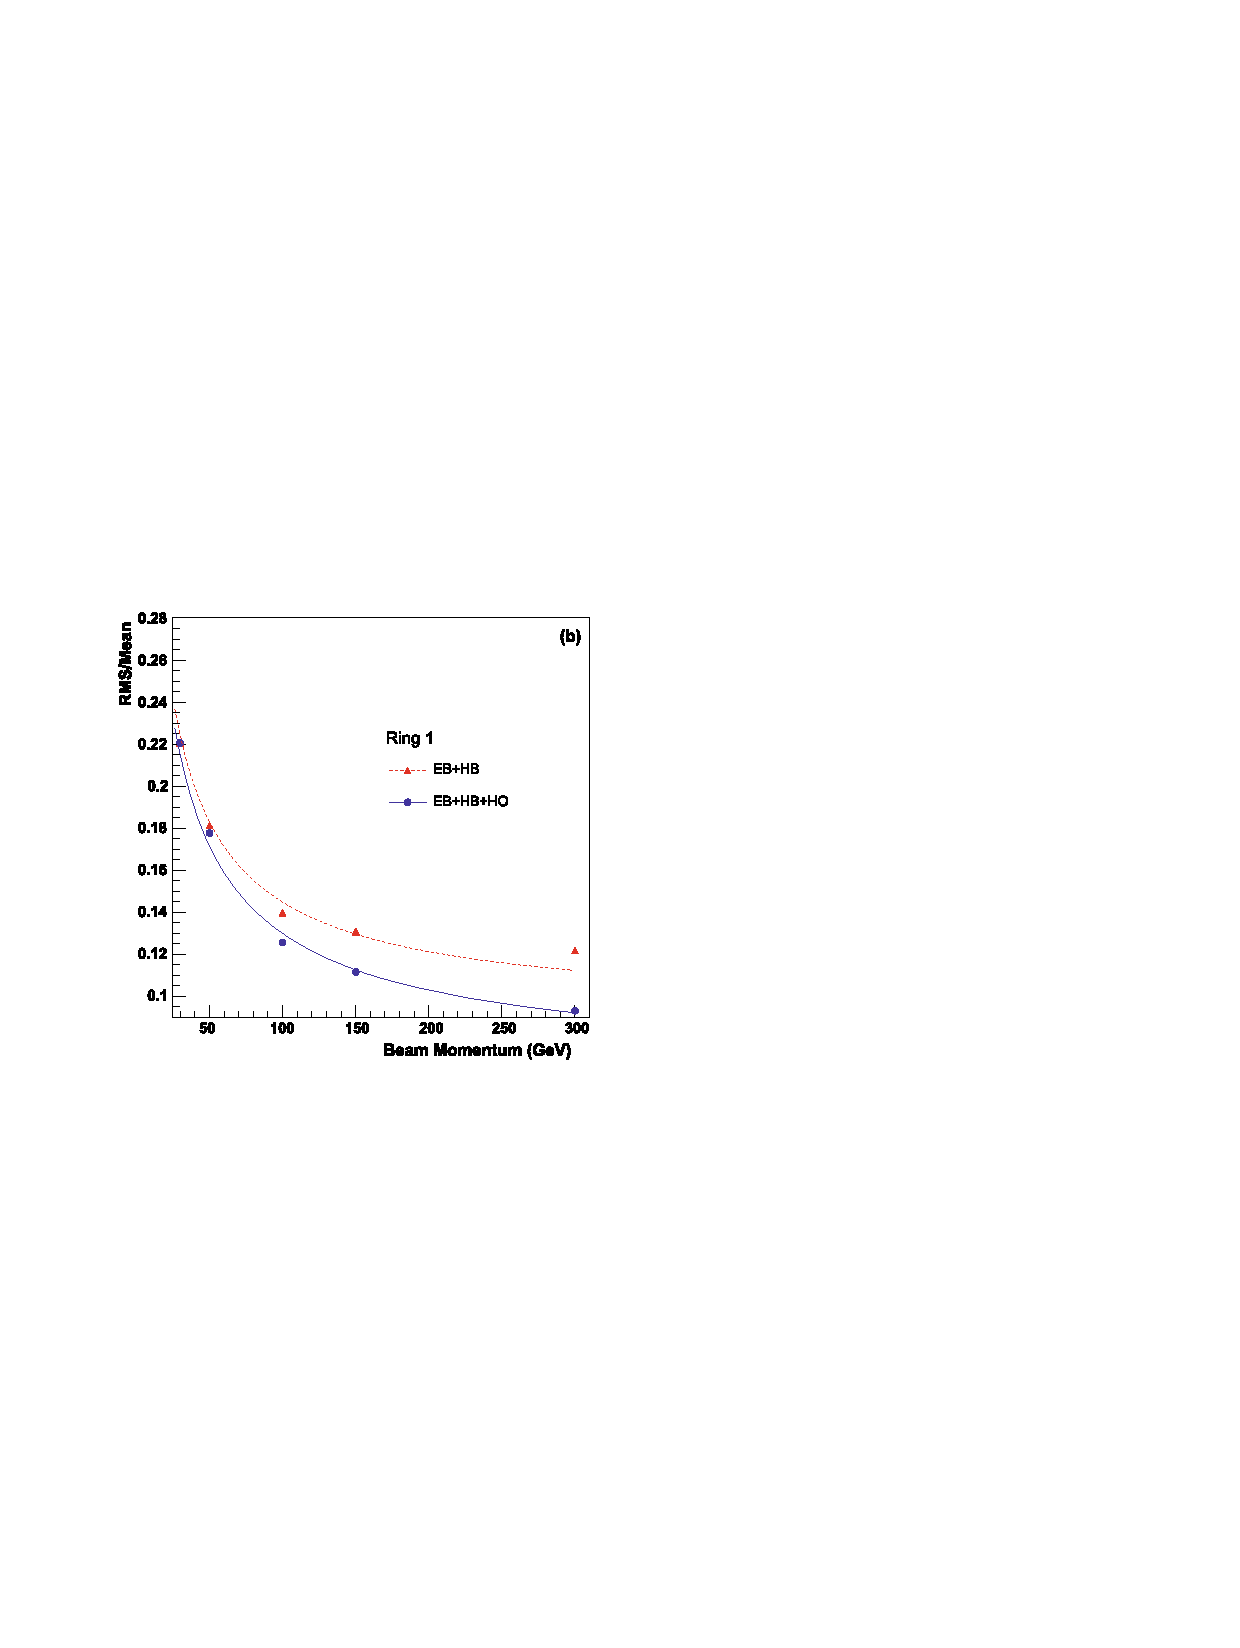
\includegraphics[width=1.2\cmsFigWidth]{figures/cms-hcal-performance2}
    \caption{Energy resolution for pions as a function of pion test-beam energy, measured for EB and HB only (red curve) and for EB, HB, and HO (blue curve)~\cite{Baiatian:951395}. The resolution visibly improves when HO energy measurements are included in the calculation. (\cmsLeft) Resolution measured for a pion beam fired at $\eta =$ 0.22. (\cmsRight) Resolution measured for a pion beam fired at $\eta =$ 0.56.}
    \label{fig:cms-hcal-performance}
  \end{center}
\end{figure}


The forward calorimeters (HF)  are located far down the beamline, with the front face of each cylinder at 11.2 m from the interaction point of the CMS detector; a cross-sectional view is shown in Figure~\ref{fig:cms-hcal-HF}. The inner radius is 12.5 cm from the beam line, and the outer radius is at 130 cm. Unlike the HB, HE, and HO, the HF calorimeters use quartz fibres rather than plastic as the scintillation medium, so as to withstand the heavy particle fluxes (an average deposited energy of 760 GeV per proton-proton interaction, compared with ~100 GeV for the rest of the HCAL) in the forward region that they occupy. Each HF cylinder is divided azimuthally into eighteen 20$^{\circ}$ wedges; the absorber is composed of 5-mm-thick steel plates with grooves into which the scintillation fibres are inserted. The absorber is subdivided into two parts in $\eta$; in one half, the fibres run through the full depth of the absorber, while in the other half, the fibres start at a depth of 22 cm from the front of the detector. With this design, the HF can distinguish between electromagnetic and hadronic showers, since the former tend to deposit most of their energy within the first 22 cm and the latter deposit nearly equal energy in both segments. 

\begin{figure}[hbtp]
  \begin{center}
    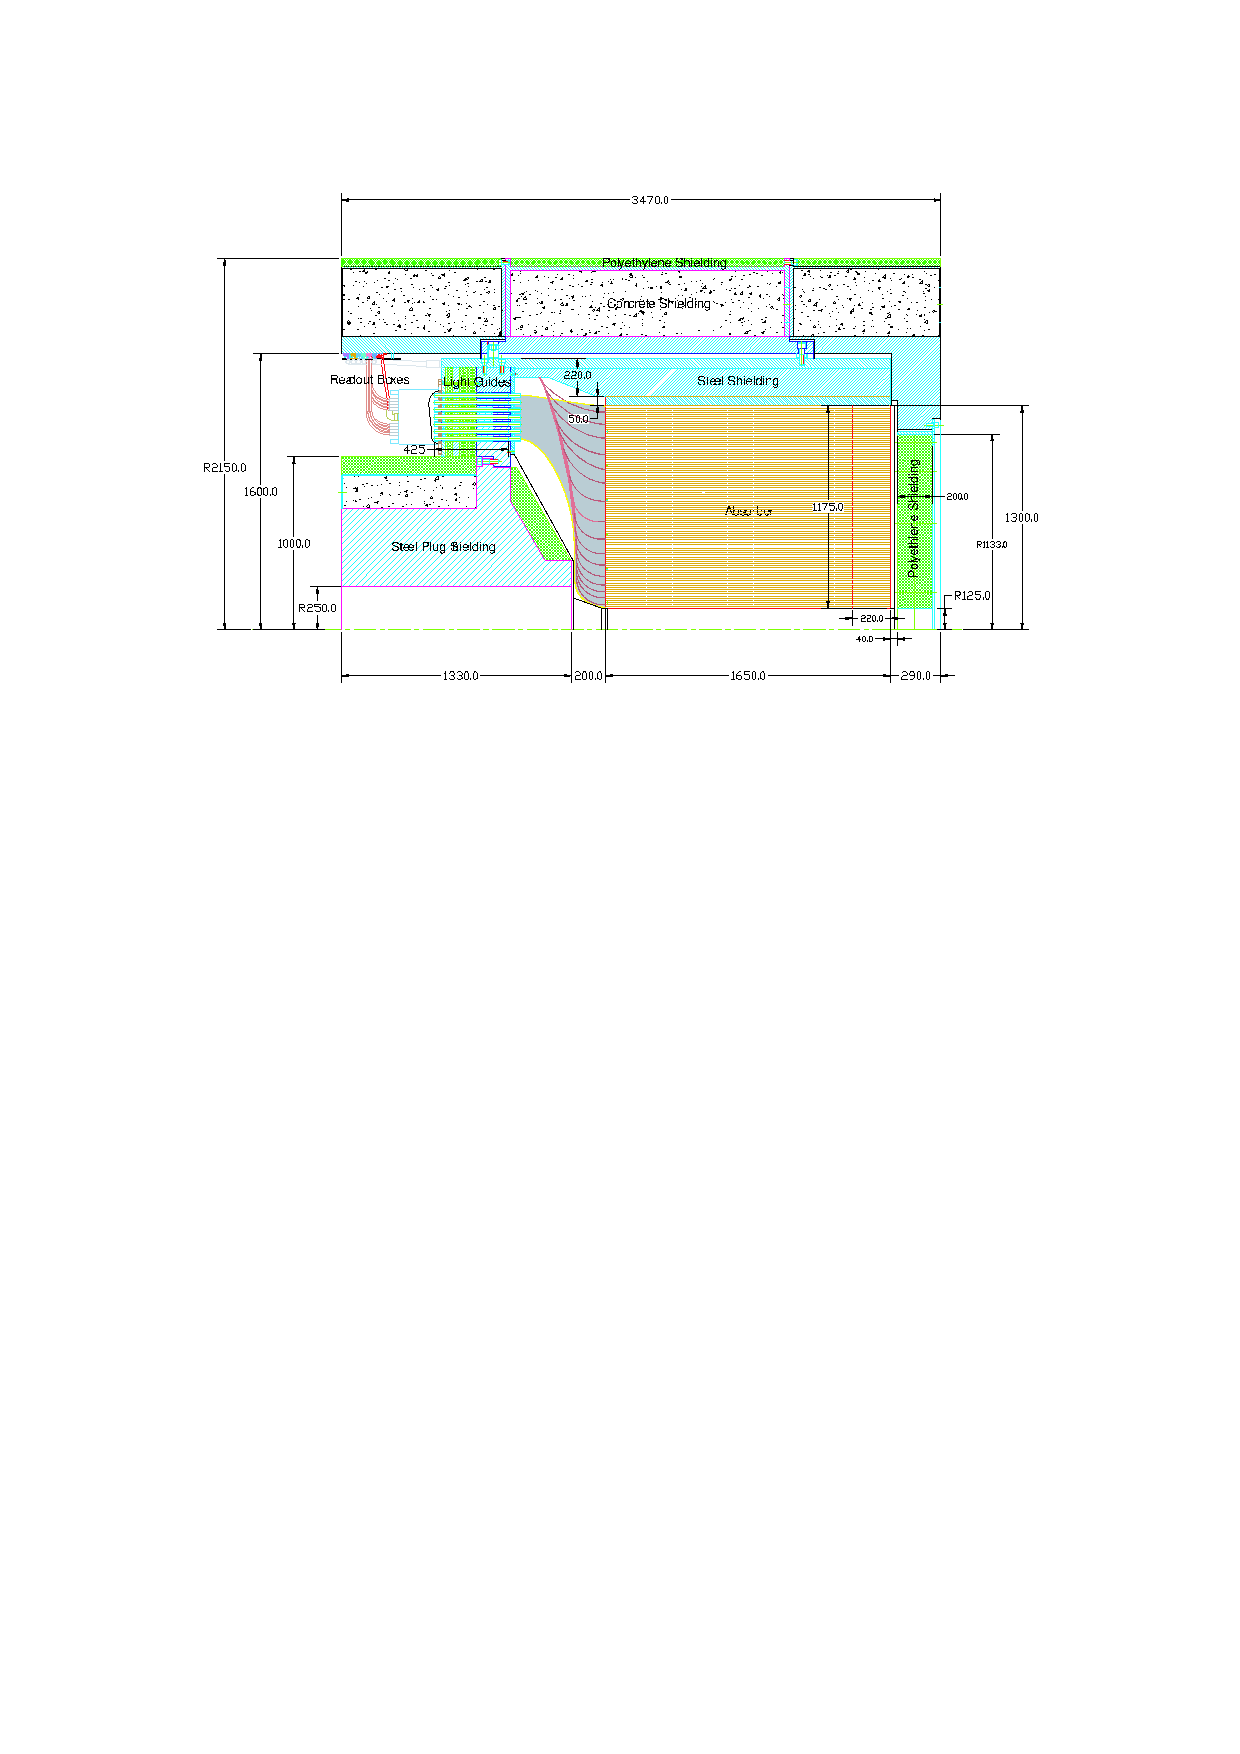
\includegraphics[width=1.5\cmsFigWidth]{figures/cms-hcal-HFxsec}
    \caption{Cross-sectional view of the HF and surrounding support structures~\cite{1748-0221-3-08-S08004}.}
    \label{fig:cms-hcal-HF}
  \end{center}
\end{figure}

The quartz fibres are made of a fused-silica core with polymer hard-cladding. Charged particles passing through the crystals with energy above the Cherenkov threshold (roughly 190 keV for electrons) will generate Cherenkov radiation, which is captured by the quartz fibres. The fraction of light $f_{trap}$ captured by a crystal is equal to NA/2n$_{core}^2$, where NA is the numerical aperture and n$_{core}$ is the refractive index of the quartz core. The light that hits the core-cladding interface at an angle larger than the critical angle of 71$^{\circ}$ can contribute to the calorimeter signal, while the rest is lost. The fibres run in bundles parallel to the beam line, forming towers with a granularity of (0.175, 0.175) in ($\eta$, $\phi$). Bundles of fibres emerging from the back of the calorimeter are routed to air-core light guides protected by a shielding matrix of steel, lead, and polyethylene. The interior of a light guide is coated with highly reflective metal and guides the received light from the quartz fibres to a photomultiplier for readout; one readout box holds 24 photomultipliers and services half of a wedge.

In addition to contributing to hadronic shower energy measurement, the HF is also used to monitor the luminosity of the LHC. The average number of empty towers in the HF is related to the mean number of interactions per bunch crossing, and there is also a linear relationship between luminosity and the average transverse energy per tower.

\subsection{Magnet\label{sec:cms-magnet}}
% solenoid, yoke, cryogenics, vacuum system

The superconducting solenoid magnet of CMS encloses the tracker detector, ECAL, and part of the HCAL inside a cylindrical bore 6.3 m in diameter and 12.5 m long, weighing 220 tonnes. The solenoid is composed of a 4-layer winding of coils made of NbTi, which is mechanically reinforced by being mixed with an aluminium alloy, an innovative method that makes the coils serve both as conductors and as their own self-stabilizing structural support.

At full current, the solenoid carries 19.14 kA, producing a nearly uniform 3.8 T magnetic field through the volume enclosed by the bore, containing 2.6 GJ of stored electromagnetic energy at full current. The magnetic flux is returned through an iron yoke, consisting of a system of barrel wheels and endcap disks arranged outside the volume of the solenoid in a cylindrical pattern and interleaved with the muon tracking system; the yoke is segmented longitudinally into 5 rings, each 2.536 m long in the z direction, with their centers positioned at z = -5.342 m, -2.686 m, 0 m, +2.686 m, and +5.342 m (rings number -2, -1, 0, 1, and 2 respectively).

\begin{figure}[hbtp]
  \begin{center}
    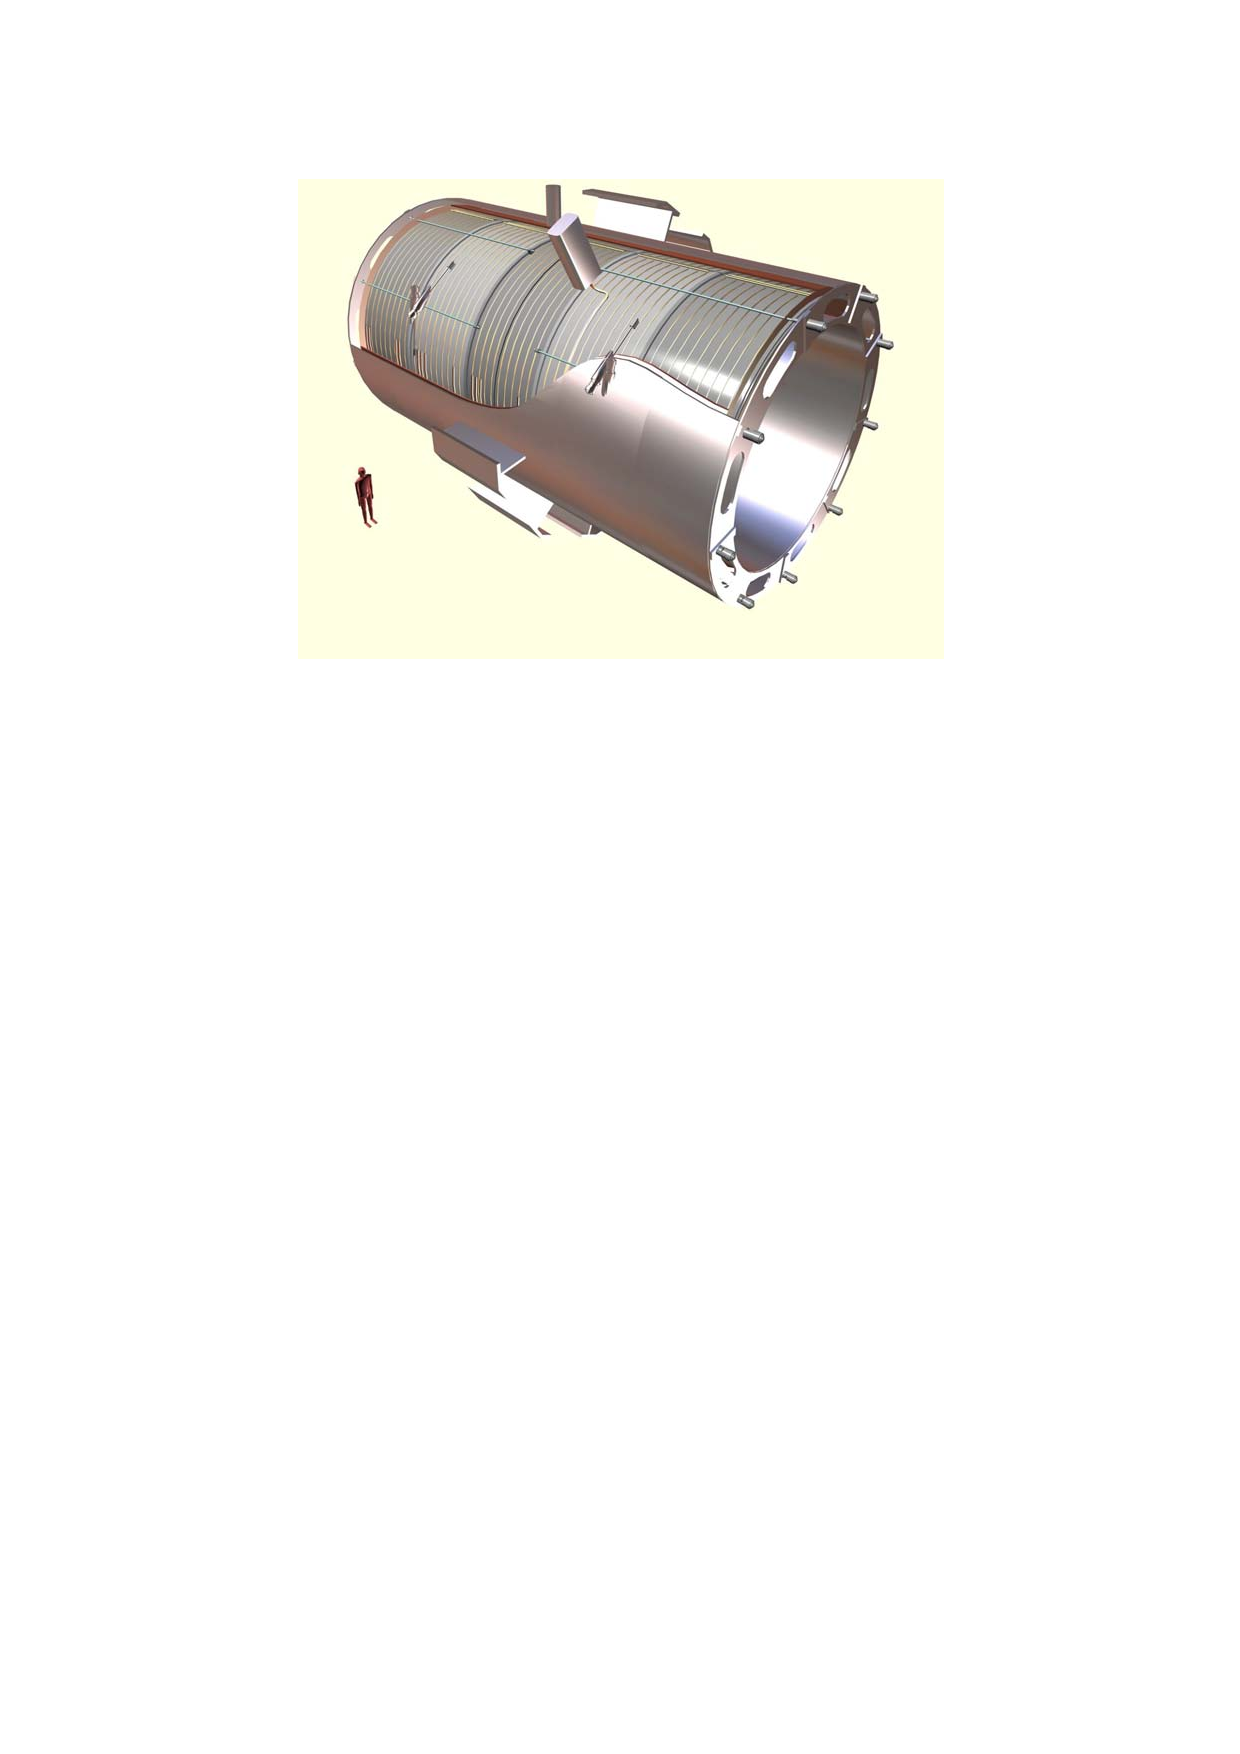
\includegraphics[width=1.24\cmsFigWidth]{figures/cms-magnetcoldmass}
    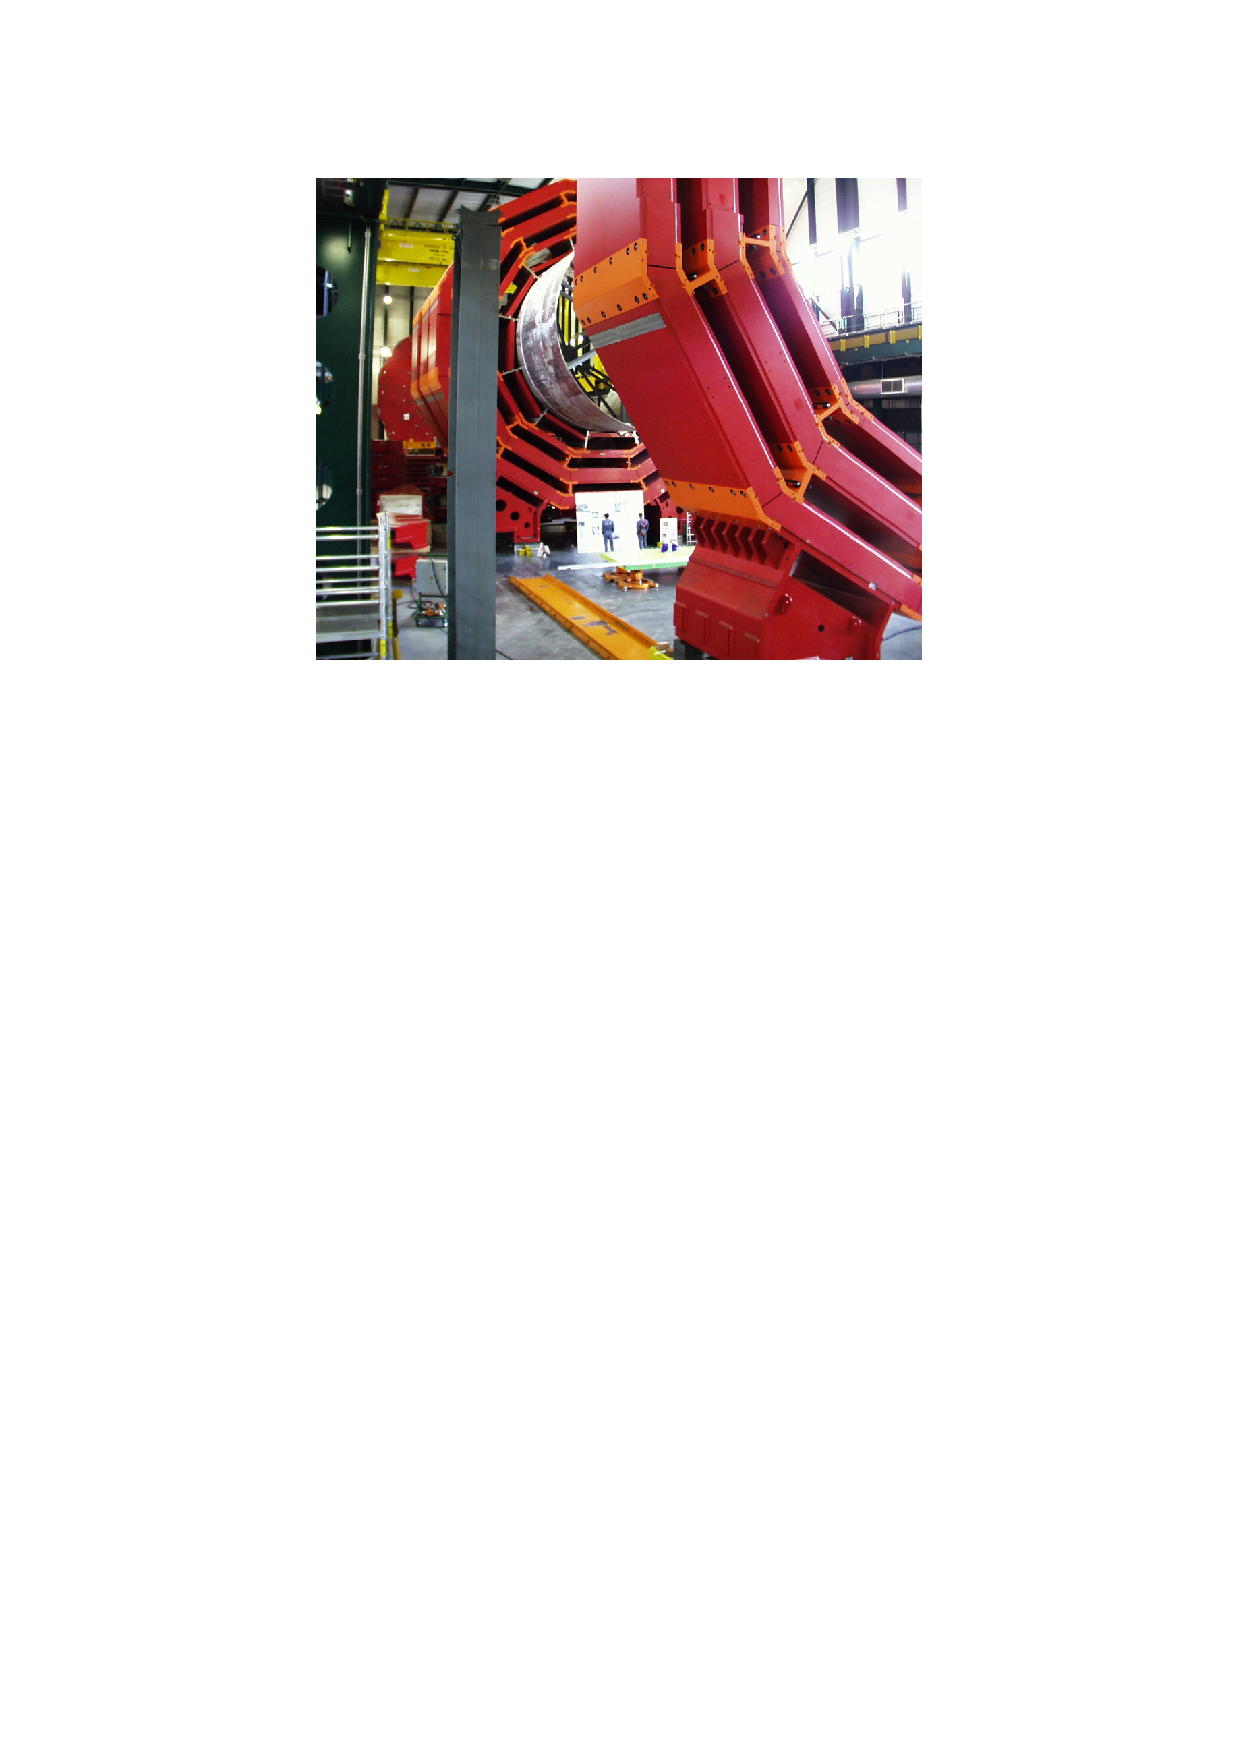
\includegraphics[width=1.24\cmsFigWidth]{figures/cms-magnetyoke}
    \caption{(\cmsLeft) Cold mass of the solenoid magnet, showing the five longitudinal segments. (\cmsRight) Image of the iron yoke of the solenoid magnet, also showing the central barrel that supports the vacuum chamber of the superconducting coil.~\cite{1748-0221-3-08-S08004}}
    \label{fig:cms-magnet}
  \end{center}
\end{figure}

\begin{figure}[hbtp]
  \begin{center}
    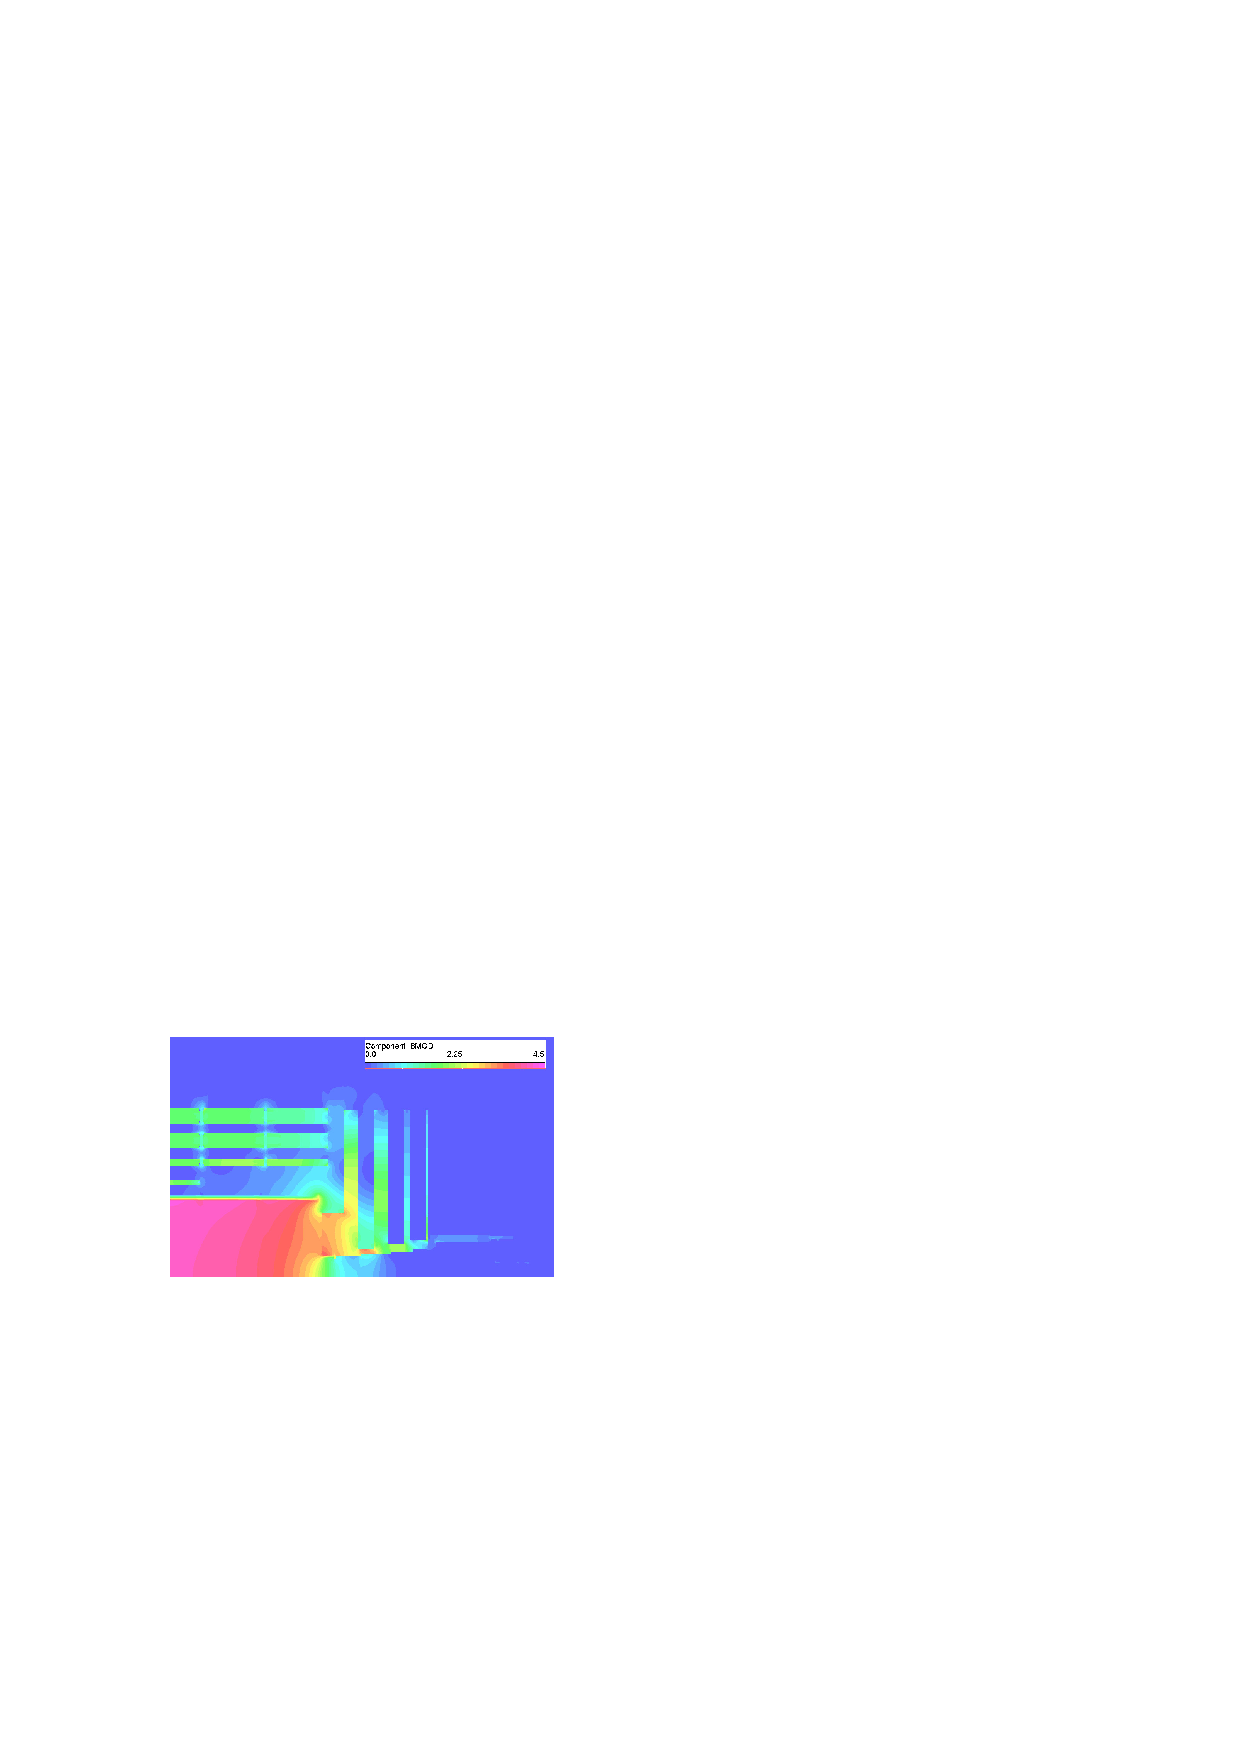
\includegraphics[width=1.24\cmsFigWidth]{figures/cms-magneticfield}
    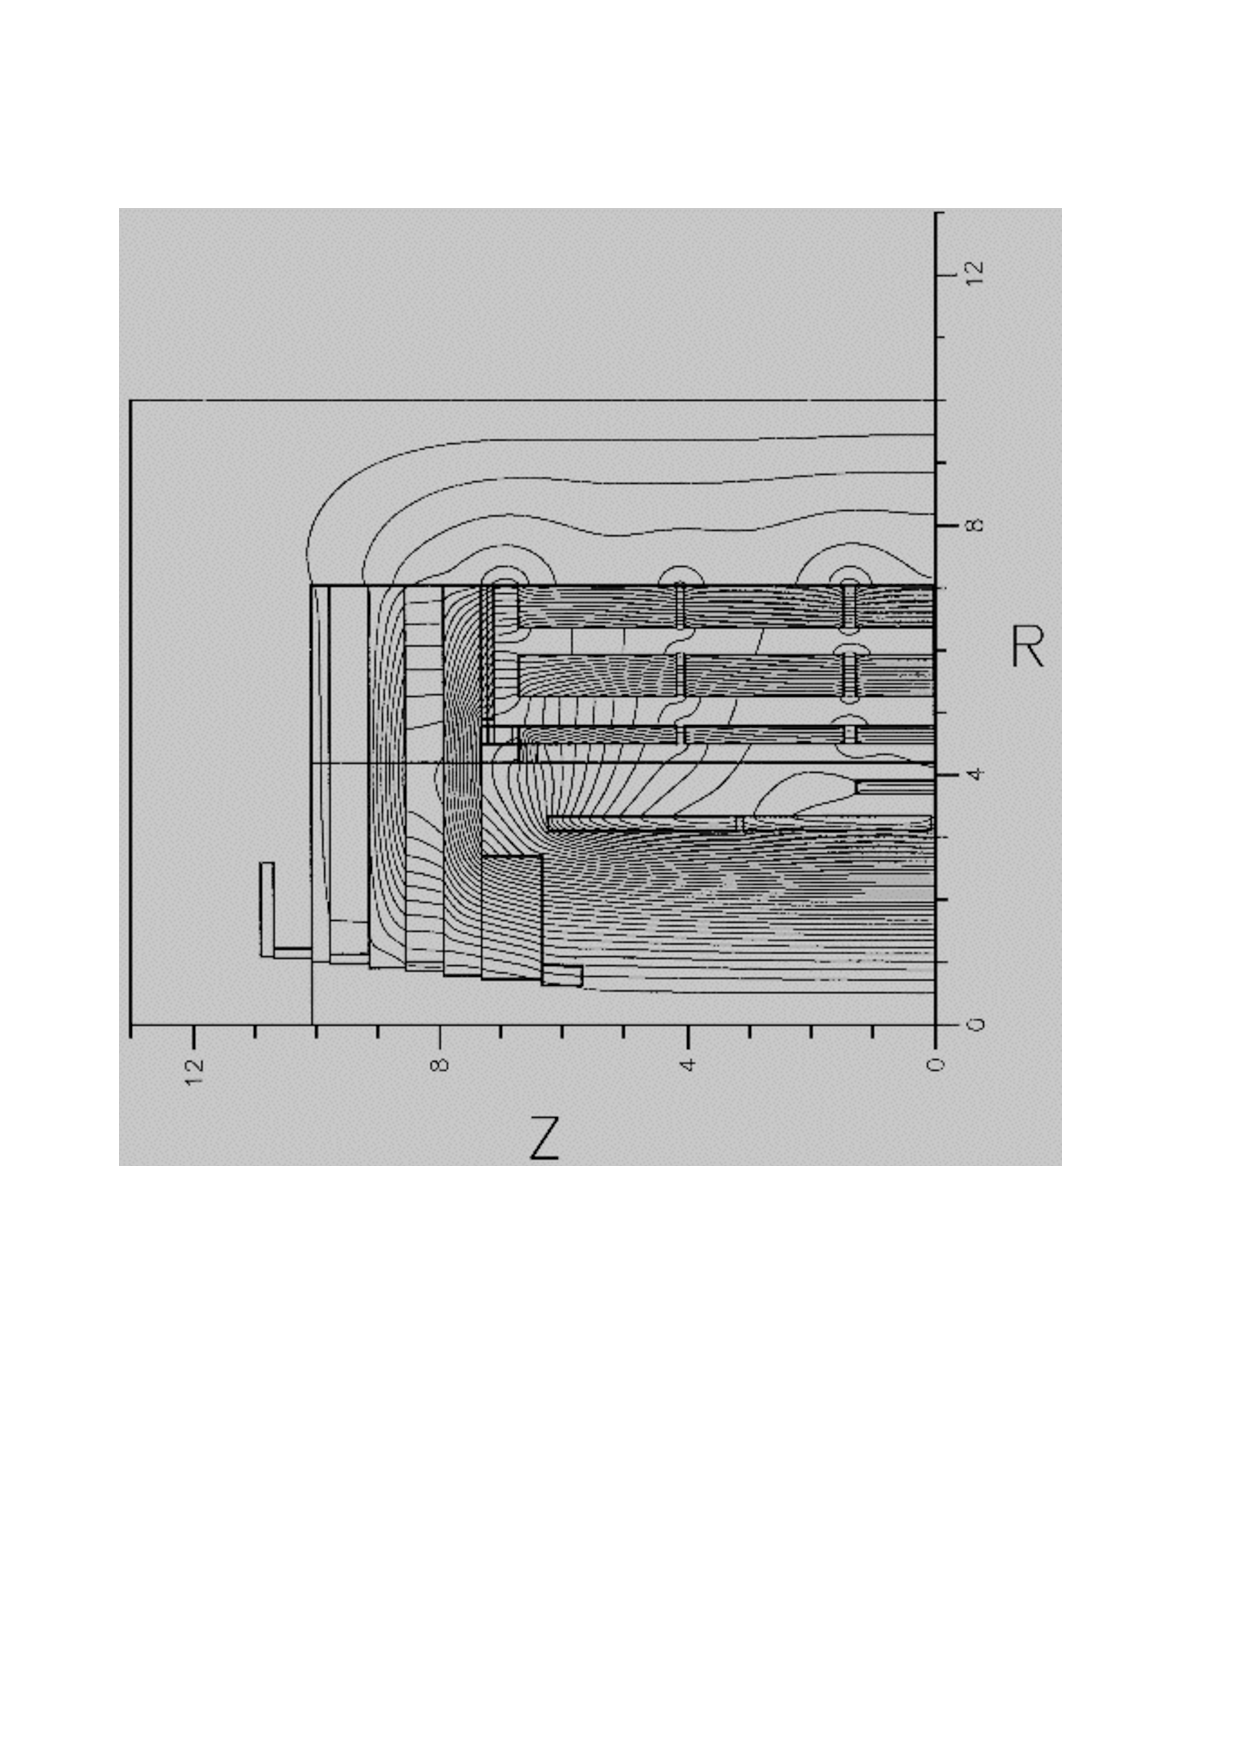
\includegraphics[width=1.24\cmsFigWidth]{figures/cms-magneticfluxinyoke}
    \caption{(\cmsLeft) Longitudinal cross-sectional view of one quarter of the CMS detector, showing a color plot of magnetic flux density (Tesla) in simulation~\cite{Amapane:883293}. (\cmsRight) Magnetic flux lines in the return yoke and muon system~\cite{Acquistapace:1997fm}.}
    \label{fig:cms-magneticfield}
  \end{center}
\end{figure}

The uniformity of the magnetic flux density inside the detector volume is illustrated in Figure~\ref{fig:cms-magneticfield}, which was obtained via simulation~\cite{Amapane:883293}. Within the solenoid volume, the field is nearly uniform at 3.8 T. The field lines becomes nonuniform at the end faces of the cylindrical solenoid volume, and the return flux is mostly confined to the iron yoke, though there is also a residual nonzero magnetic flux in the muon system volume.

\subsection{Muon system\label{sec:cms-muon}}
% DT, CSC, RPC, readouts for all
  
Muons tend to undergo far lower radiative losses in detector material than electrons with similar kinetic energy and are consequently cleaner to reconstruct. Because they are expected to be the only particles (not counting neutrinos) that survive past the tracker and calorimeter layers, the muon detector system is the outermost layer of the CMS detector, located outside the solenoid. Muons are part of many of the physics signatures sought at the LHC, such as the decay $H\rightarrow$$ZZ*\rightarrow$$4\mu$ or $H\rightarrow WW/ZZ$, and so the experiment benefits from having a muon system with wide angular coverage and efficienct reconstruction capabilities.

Like the rest of the CMS subsystems, the muon system is comprised of a barrel region and two endcap regions. The muon detector chambers are mounted on the flux return yoke system. The barrel is made of four layers called stations, and its longitudinal segmentation is dictated by the segmentation of the yoke into 5 rings, while the azimuthal segmentation comes from the iron ribs of the yoke that serve as support structures for the solenoid coil cryostat and the HCAL outer calorimeter~\cite{MuonTDR}.

The goals of the muon system are to provide reliable reconstruction of muon momentum and charge over the entire kinematic range of the LHC, as well as to provide the capability to trigger on events in the detector (the concept of triggering is explained in Section~\ref{sec:cms-triggerdaq}). To these ends, the muon system employs three different kinds of gas ionization detector technology: drift tubes (DTs), cathode strip chambers (CSCs), and resistive plate chambers (RPCs).

The DT system is located only in the barrel of the muon detector. The choice to use DTs was based on the low expected particle flux and low magnetic field in the barrel. The smallest sensitive element is the drift cell, with a transverse dimension of 21 mm and an anode wire of roughly 2.4 m in length. Figure~\ref{fig:cms-muon-DTcell} shows a cross-section of a DT cell. The cells contain an 85\%:15\% mixture of Argon and CO$_2$ gas; when a charged particle passes through, the ionization of the gas results in a charge carrier cascade that is picked up by the anode and cathode wires and amplified by the readout system.

\begin{figure}[hbtp]
  \begin{center}
    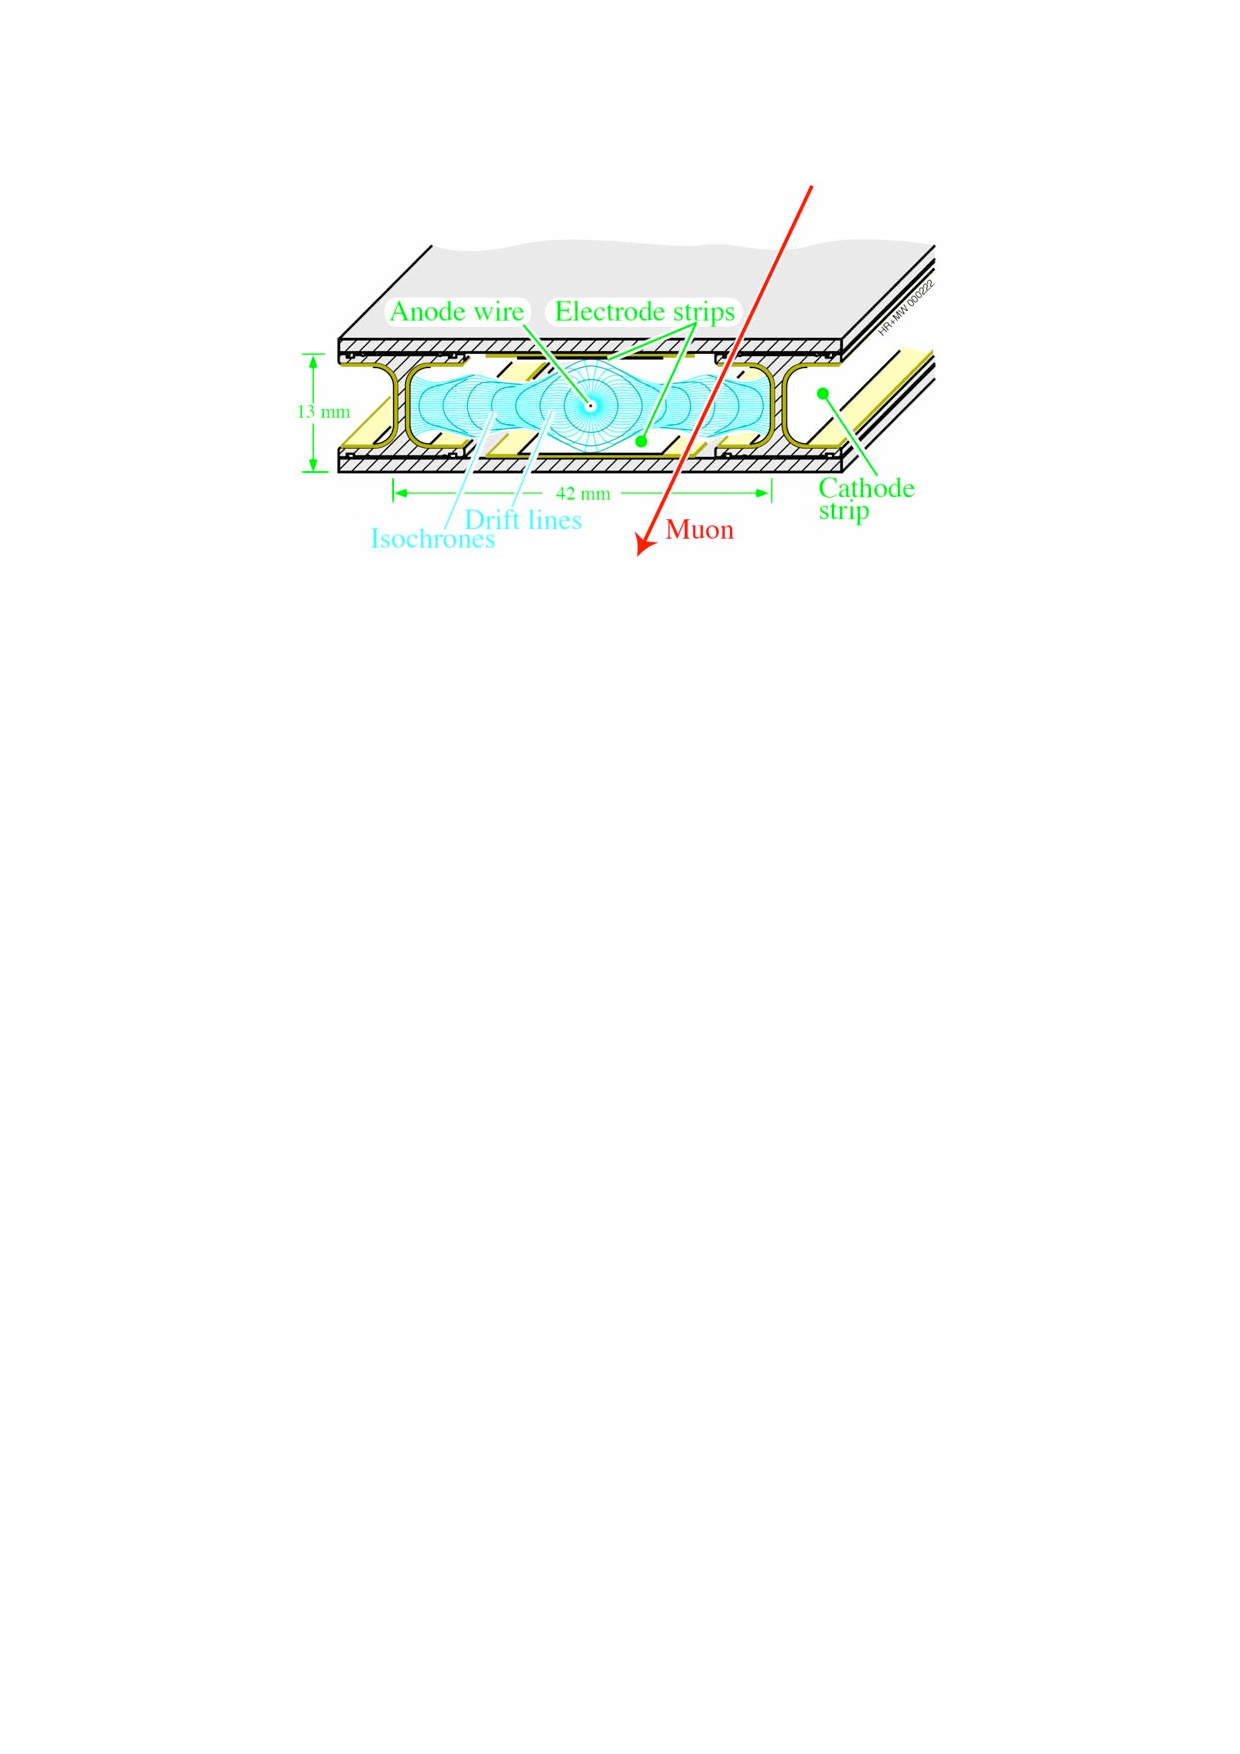
\includegraphics[width=1.5\cmsFigWidth]{figures/cms-muon-DTcell}
    \caption{Cross-sectional view of a DT cell, with drift lines indicated~\cite{1748-0221-3-08-S08004}.}
    \label{fig:cms-muon-DTcell}
  \end{center}
\end{figure}

\begin{figure}[hbtp]
  \begin{center}
    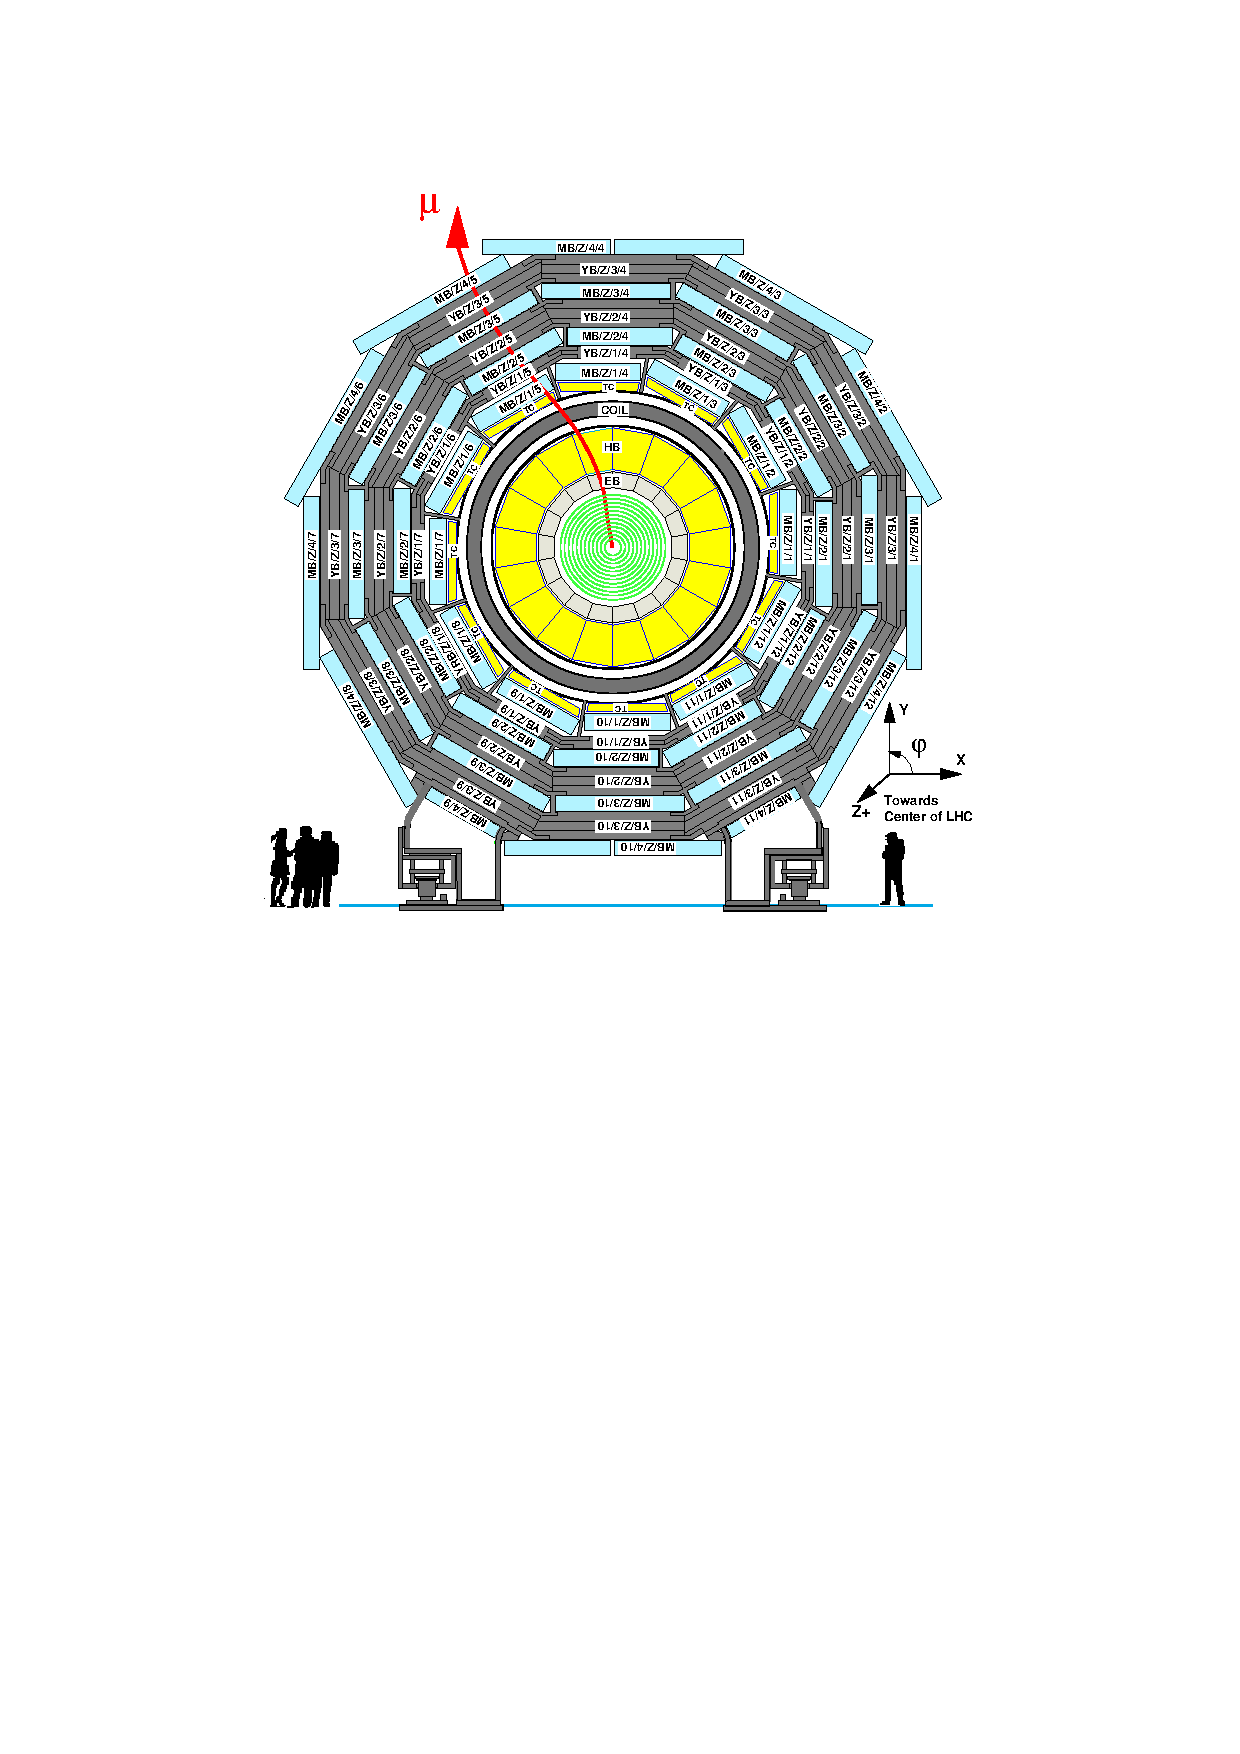
\includegraphics[width=1.5\cmsFigWidth]{figures/cms-muon-DTlayout}
    \caption{Layout of the DT chambers (light blue) in the iron yoke~\cite{1748-0221-3-08-S08004}.}
    \label{fig:cms-muon-DTlayout}
  \end{center}
\end{figure}

Drift cells are grouped into four layers staggered by half a cell; these groups of four layers are independent units known as superlayers (SLs). SLs are further grouped into groups of either 2 or 3 to form a drift chamber. Drift chambers with only SL's have wire anodes running only in the r-$\phi$ direction and provide only a measurement of the $\phi$ coordinate of a hit; these chambers are only located in the fourth muon station. In the inner three muon stations, the chambers are composed of 3 SL's, of which the outermost two have wire anodes running in the r-$\phi$ direction and the other has the wire running in the z direction, thus yielding both r-$\phi$ and z coordinates of a hit. The inner three muon stations have 60 drift tube chambers each, while the fourth station has 70; Figure~\ref{fig:cms-muon-DTlayout} depicts the layout of the DT chambers mounted in the iron yoke.

\begin{figure}[hbtp]
  \begin{center}
    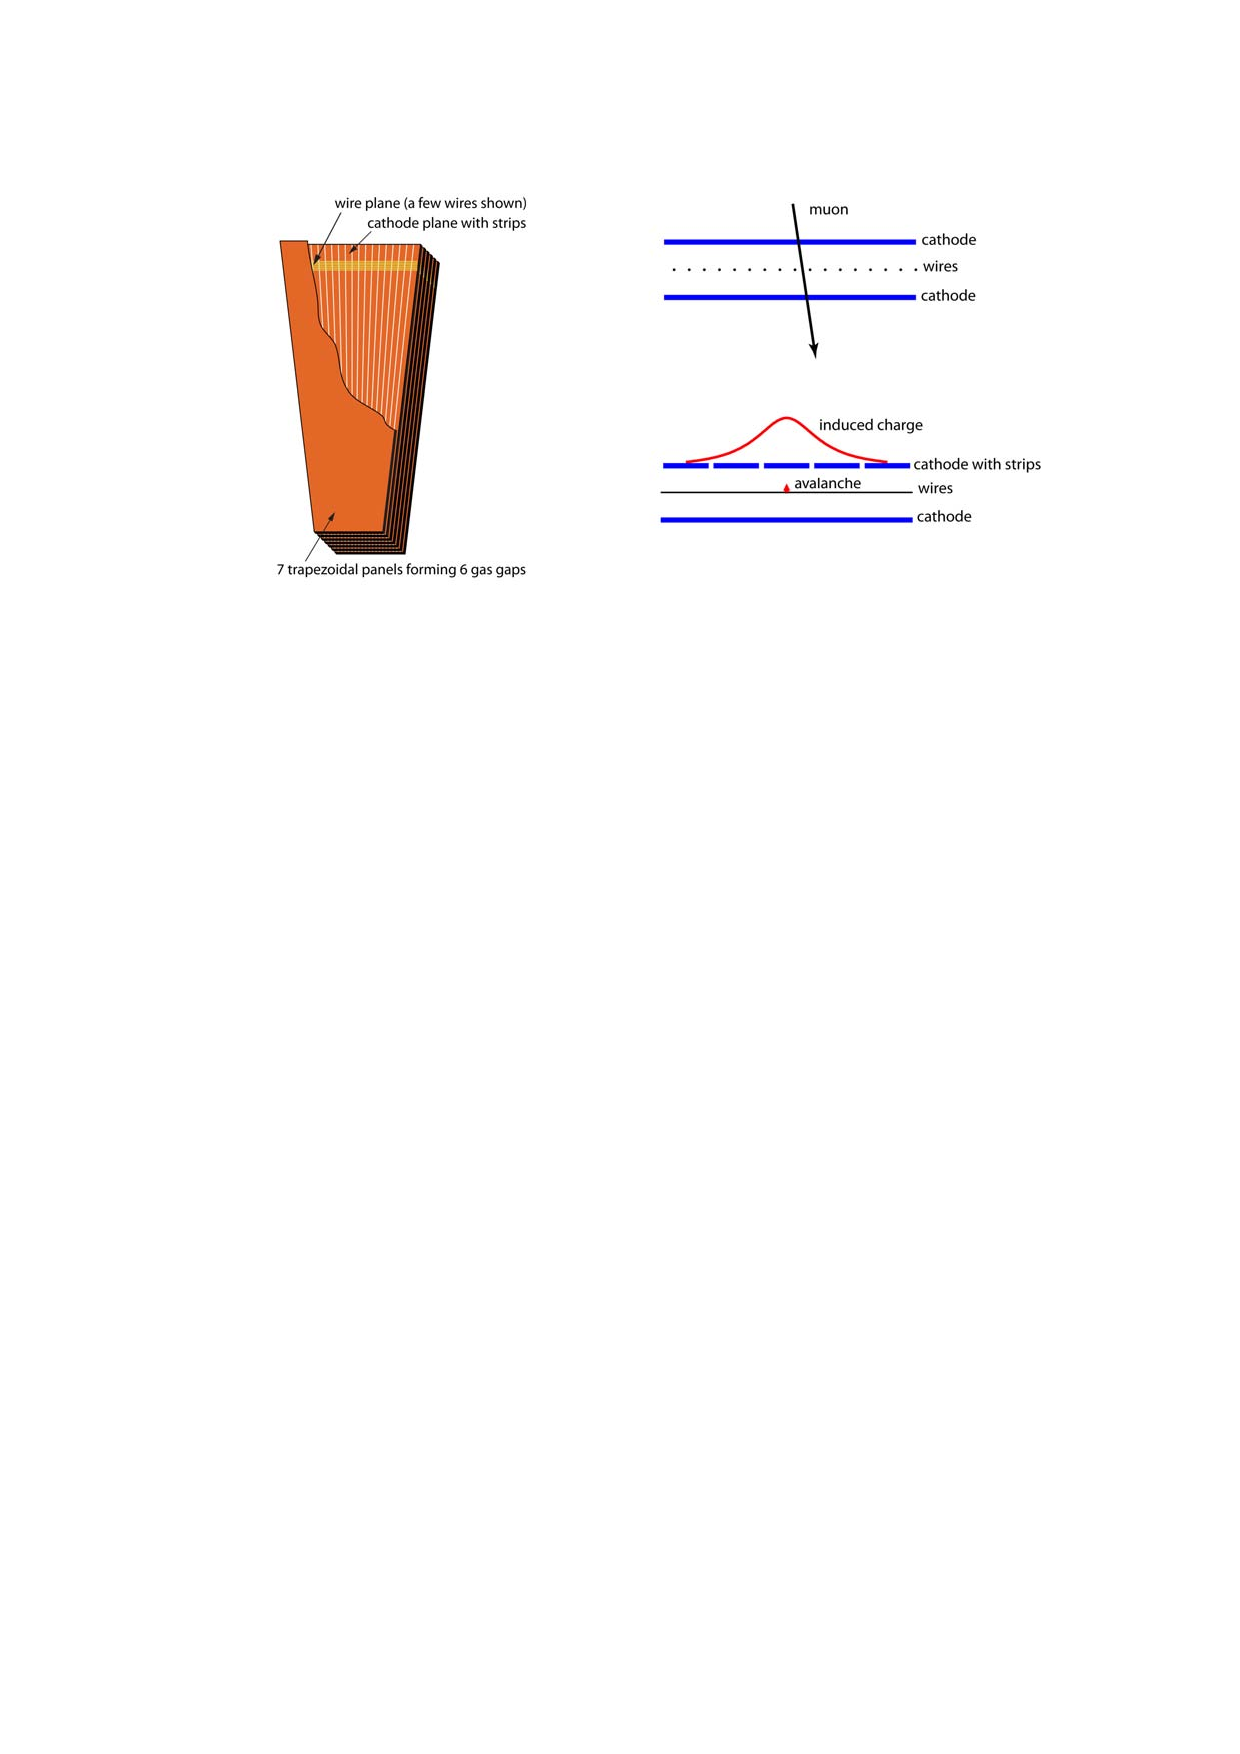
\includegraphics[width=1.24\cmsFigWidth]{figures/cms-muon-CSCcell}
    \caption{(\cmsLeft) Layout of a CSC, with the top panel peeled back to show anode wires and cathode strips. (\cmsRight) Diagram of charge induction in a CSC gap by a passing high-energy particle. By the same logic as for charge sharing in the pixel system, the interpolation of charges induced on cathode strips by an avalanche of positive charge carriers near a wire leads to better resolution of the avalanche position along the wire direction~\cite{1748-0221-3-08-S08004}}
    \label{fig:cms-muon-CSCcell}
  \end{center}
\end{figure}

\begin{figure}[hbtp]
  \begin{center}
    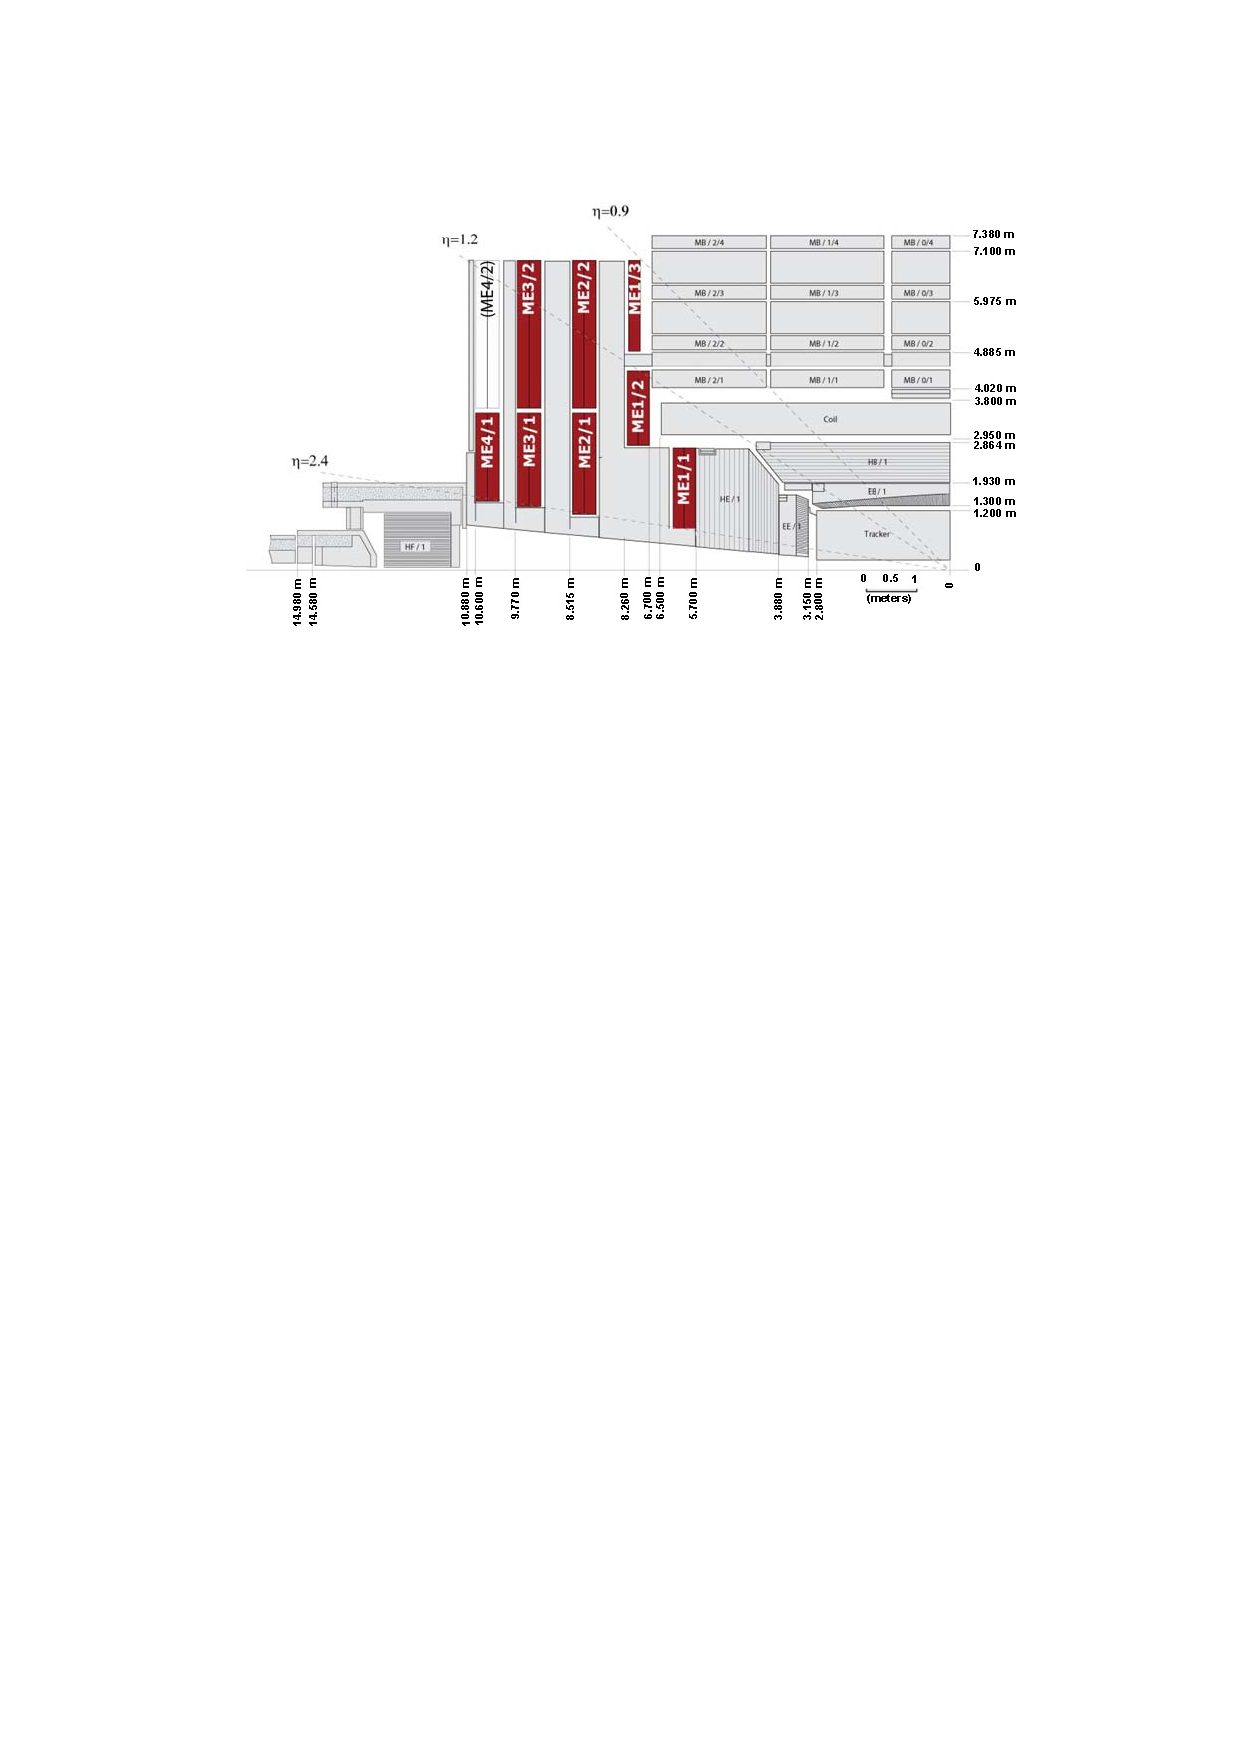
\includegraphics[width=1.24\cmsFigWidth]{figures/cms-muon-CSClayout}
    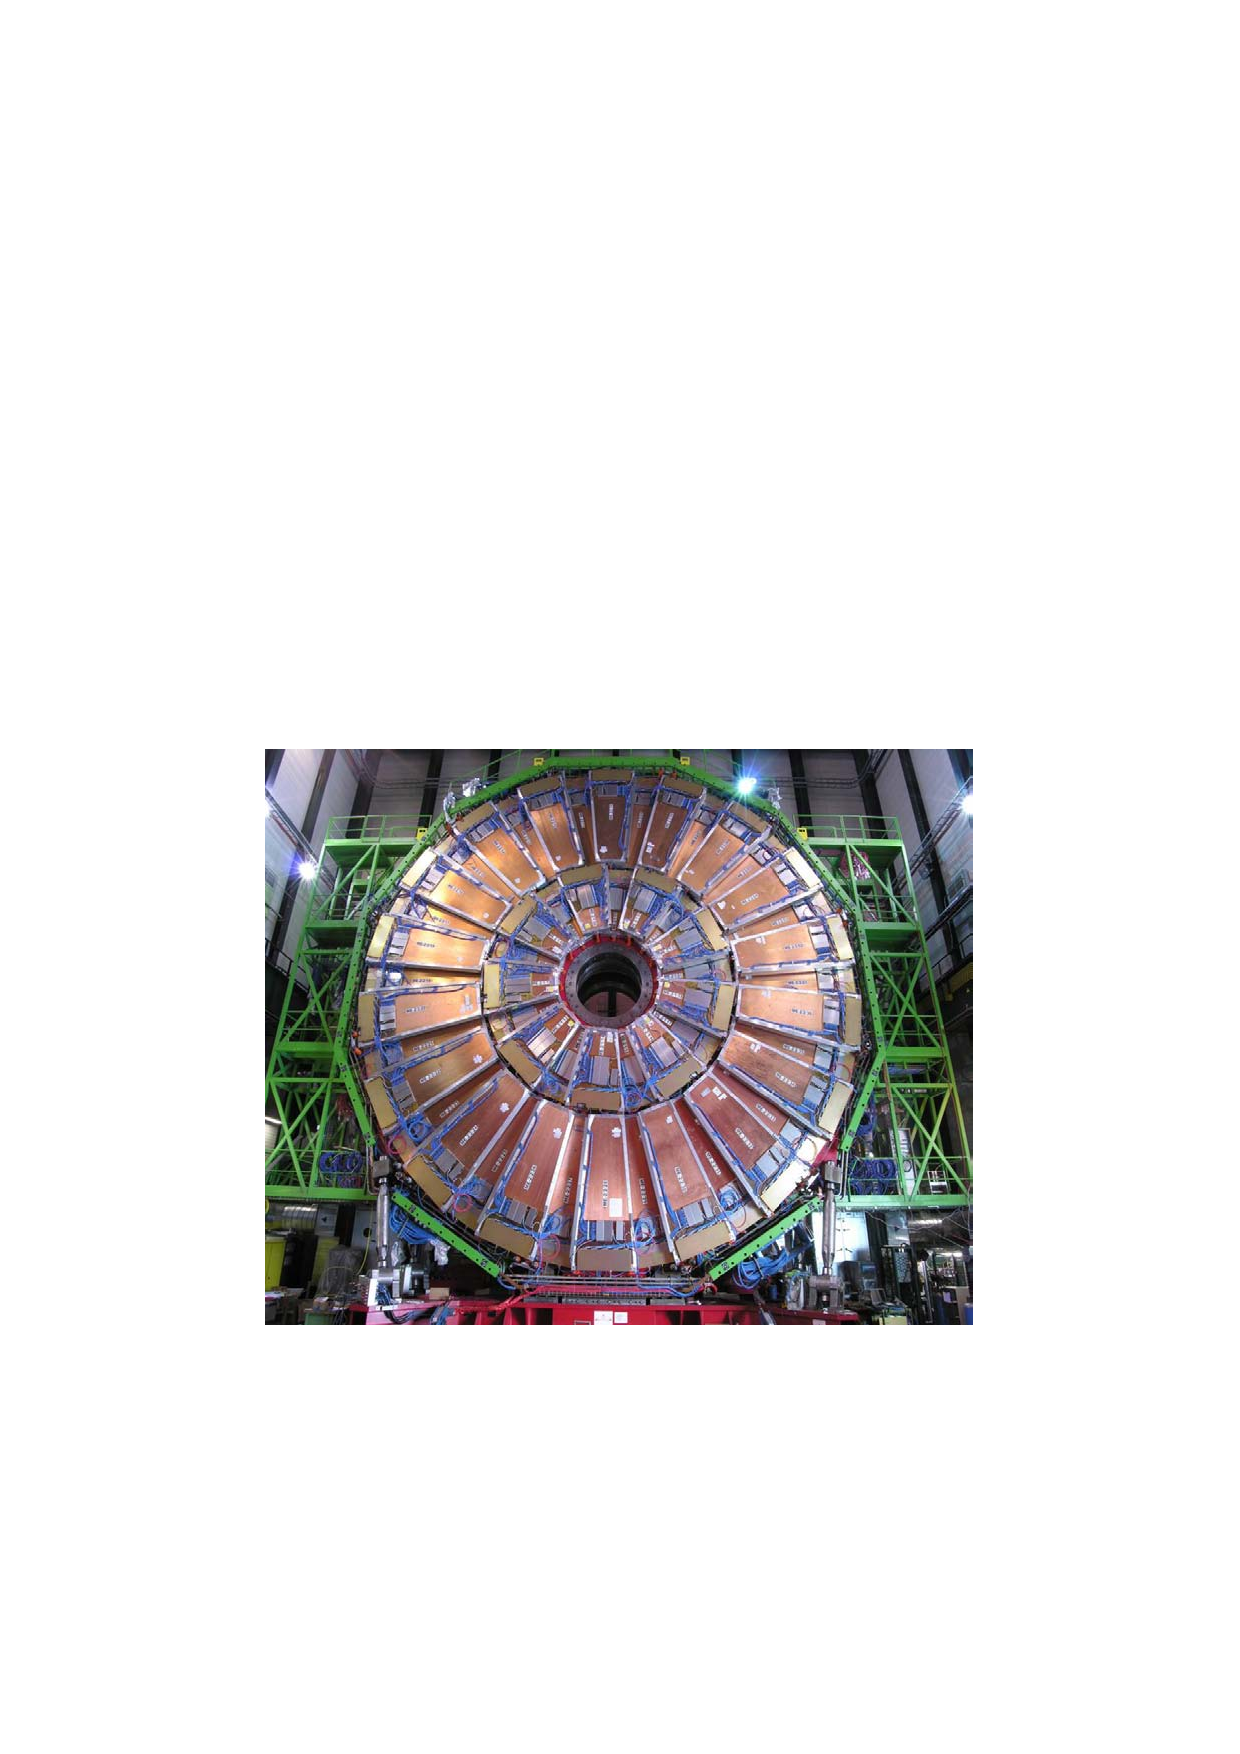
\includegraphics[width=1.24\cmsFigWidth]{figures/cms-muon-CSCchambers}
    \caption{(\cmsLeft) View of the CSC chambers (dark red) in the CMS detector. (\cmsRight) Photo of one of the CSC stations. The chambers in each ring (inner and outer) overlap to provide continous azimuthal coverage.~\cite{1748-0221-3-08-S08004}}
    \label{fig:cms-muon-CSClayout}
  \end{center}
\end{figure}

CSCs were chosen for the endcap region of the muon detector where the particle flux is higher. The cathode strip chambers are trapezoidal multi-wire proportional counters, with 6 anode wires running along the azimuthal direction and 7 cathode strips running perpendicular to the wires in the radial direction. Thus, the passage of a particle through a CSC will yield a measurement in both r and $\phi$ coordinates (from the charges induced in the anode and cathode strips respectively), with spatial resolution within 80 $\mu$m. The shape and structure of a CSC are shown in Figure~\ref{fig:cms-muon-CSCcell}, as well as a depiction of charge induction on cathode strips in a CSC.

There are 468 cathode strip chambers in total, providing coverage over the pseudorapidity range 0.9 $< \abs{\eta} <$ 2.4. The gas used in the chambers is a mixture of argon, CO$_2$, and CF$_4$ in a ratio of 40\%:50\%:10\%, with the CF$_4$ included to prevent polymerization on the wires. The CSC system has two purposes: to yield a precise measurement of muon tracks, and to provide information for triggering. Local charged track (LCT) boards sample all the anode and cathode strip readouts of all chambers in synchronization with every LHC bunch crossing. Algorithms seek patterns of hits in the output read out by the anode and cathode LCT boards; if patterns are found that are consistent with muon tracks, they serve as trigger primitives and are used for building muon track candidates.

\begin{figure}[hbtp]
  \begin{center}
    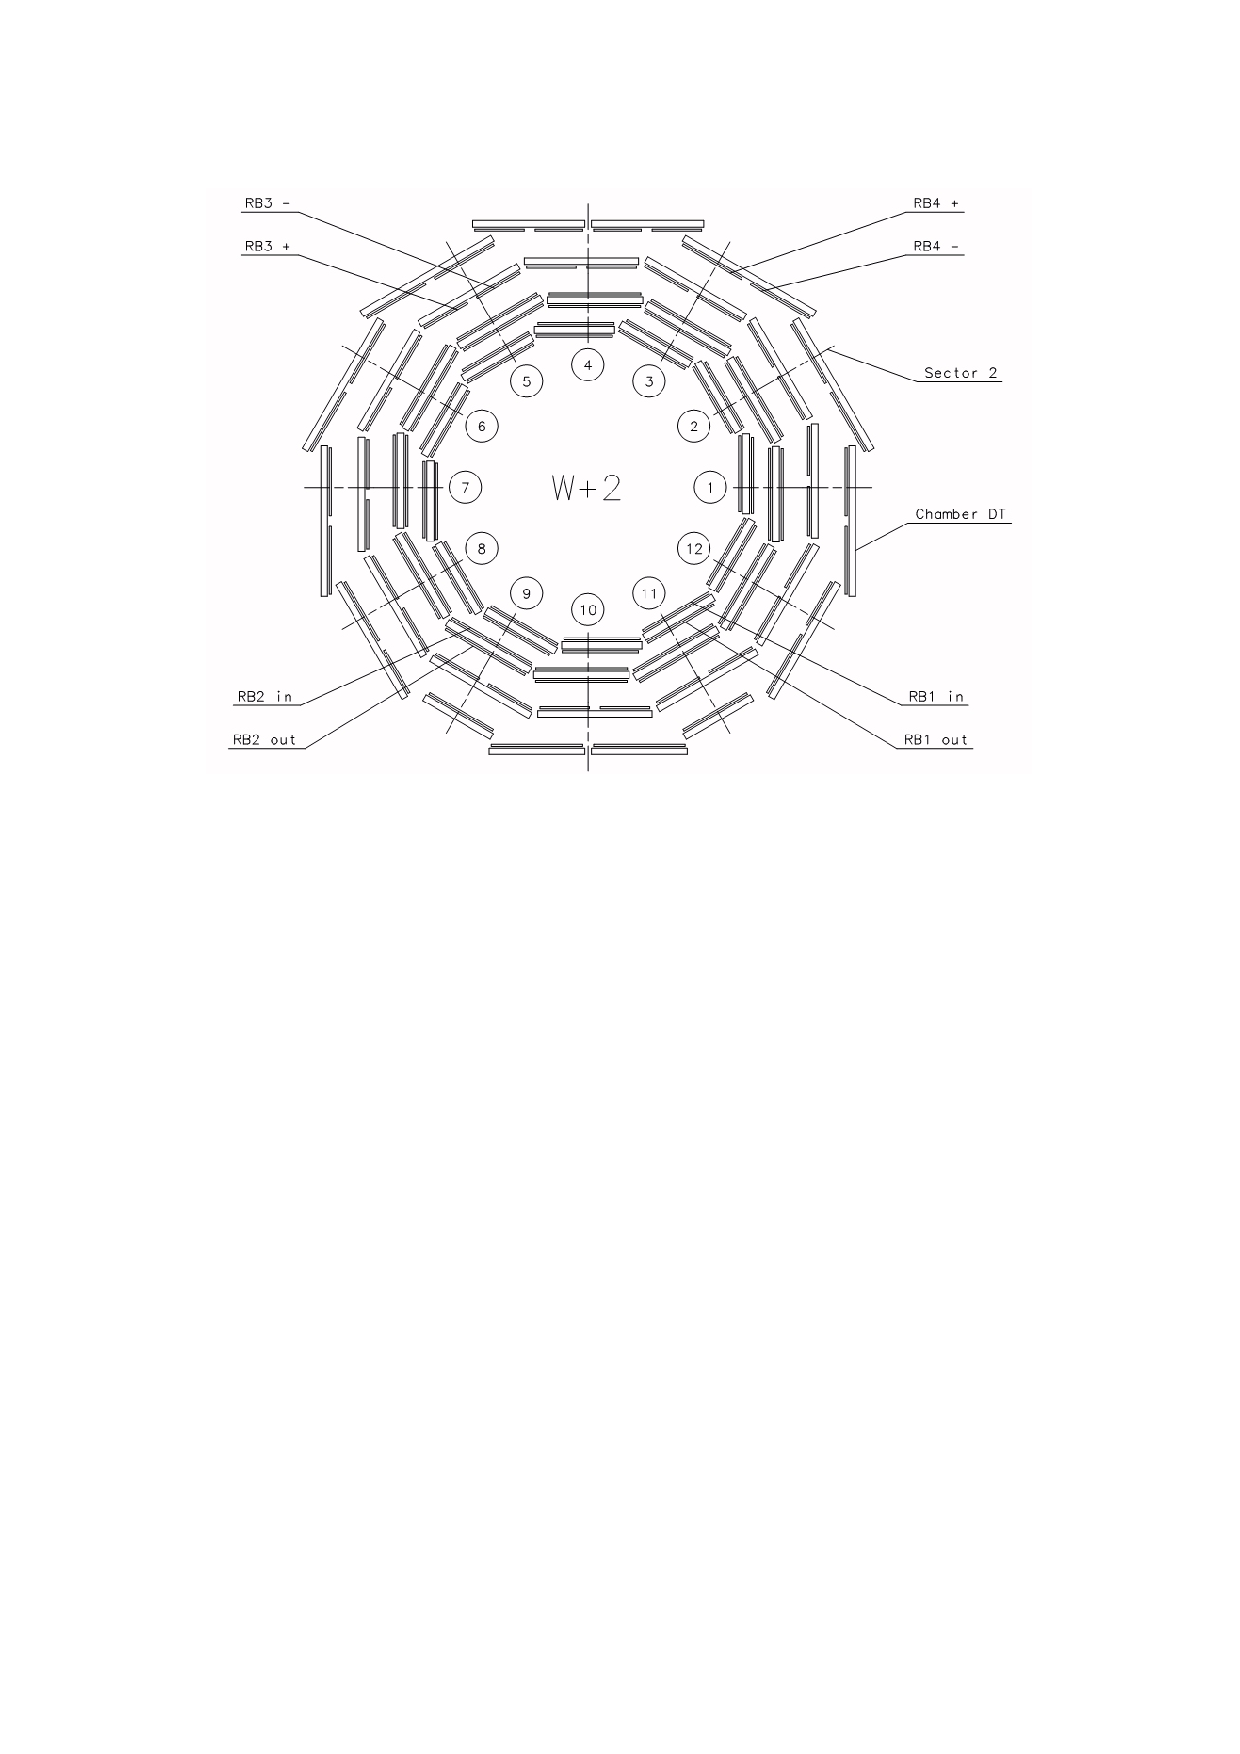
\includegraphics[width=1.24\cmsFigWidth]{figures/cms-muon-RPCbarrellayout}
    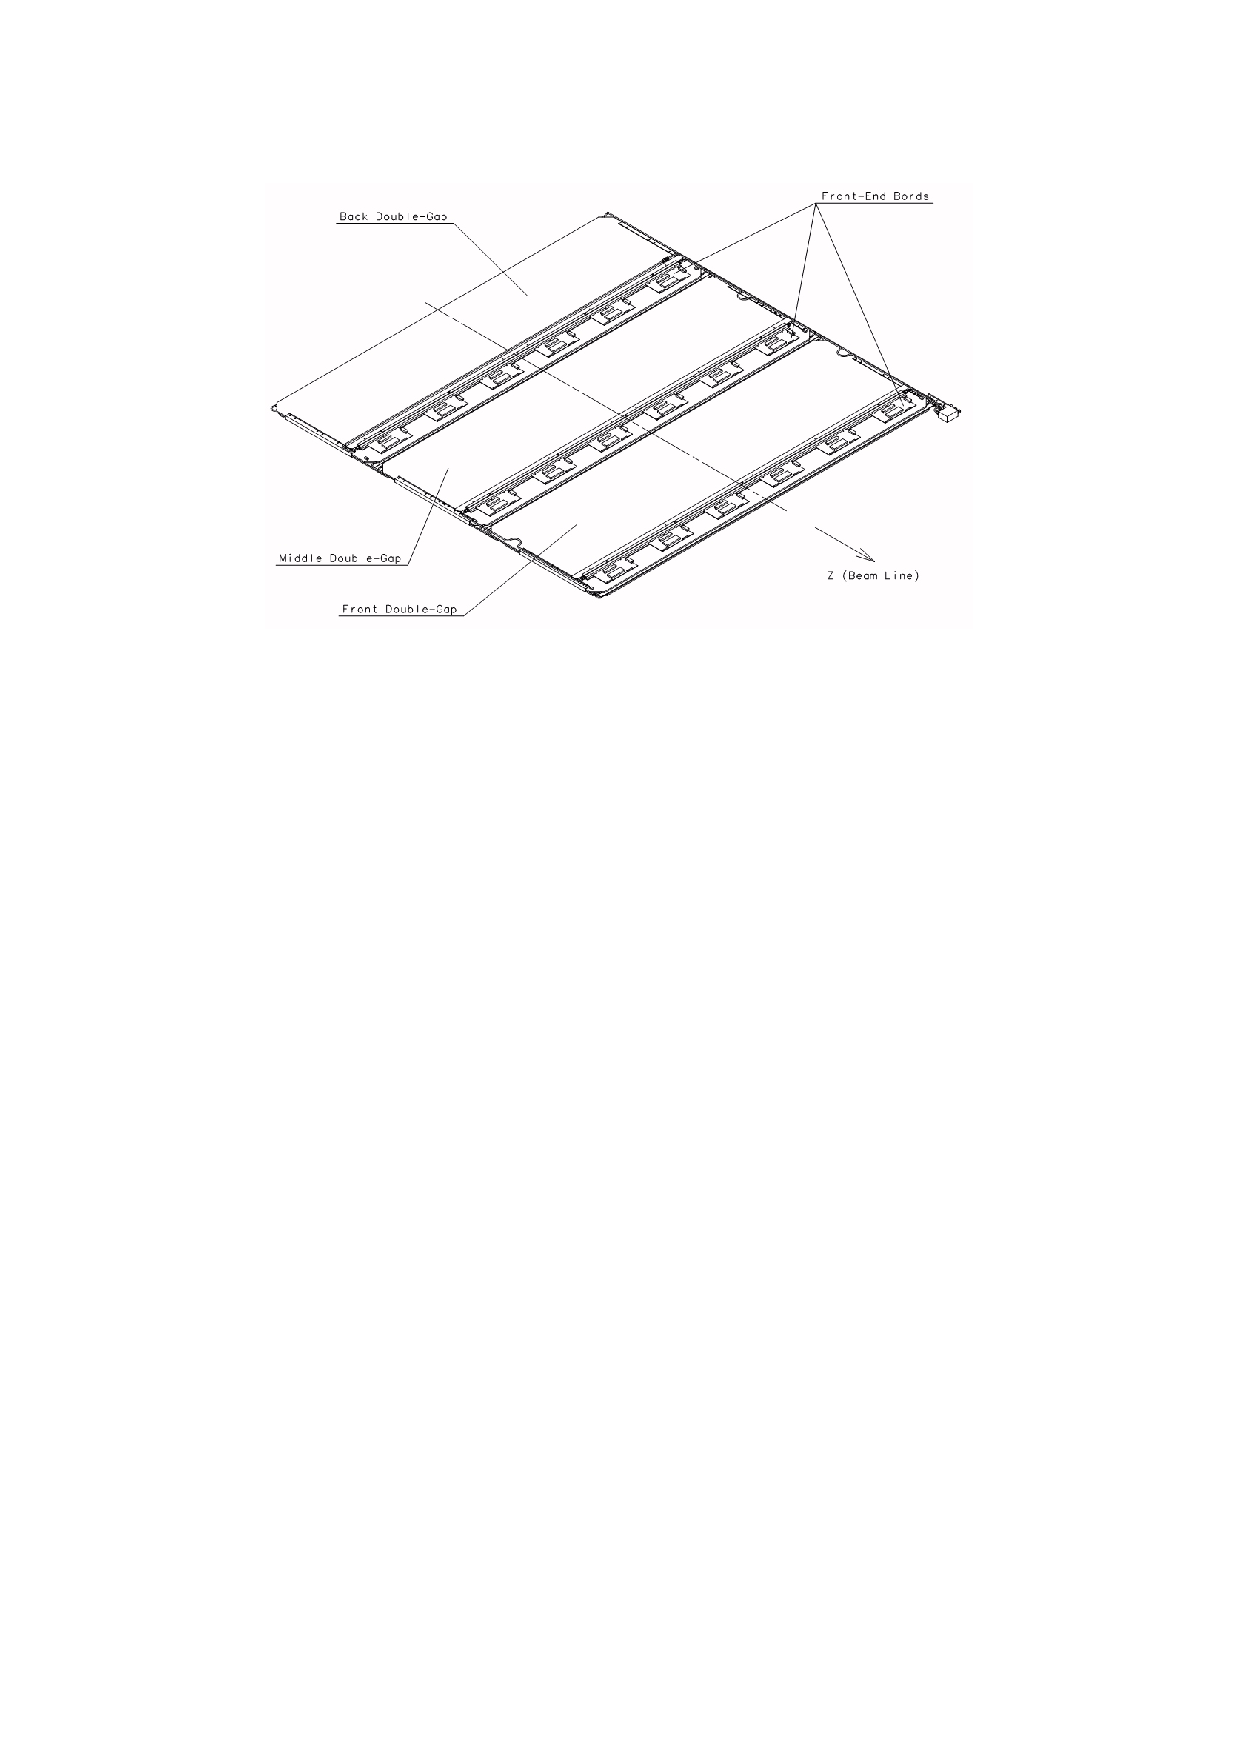
\includegraphics[width=1.24\cmsFigWidth]{figures/cms-muon-RPCmodule3}
    \caption{(\cmsLeft) Layout of the RPC barrel (dark grey) in the iron yoke. (\cmsRight) Barrel RPC module with 3 double-gaps.~\cite{1748-0221-3-08-S08004}}
    \label{fig:cms-muon-RPCbarrel}
  \end{center}
\end{figure}

\begin{figure}[hbtp]
  \begin{center}
    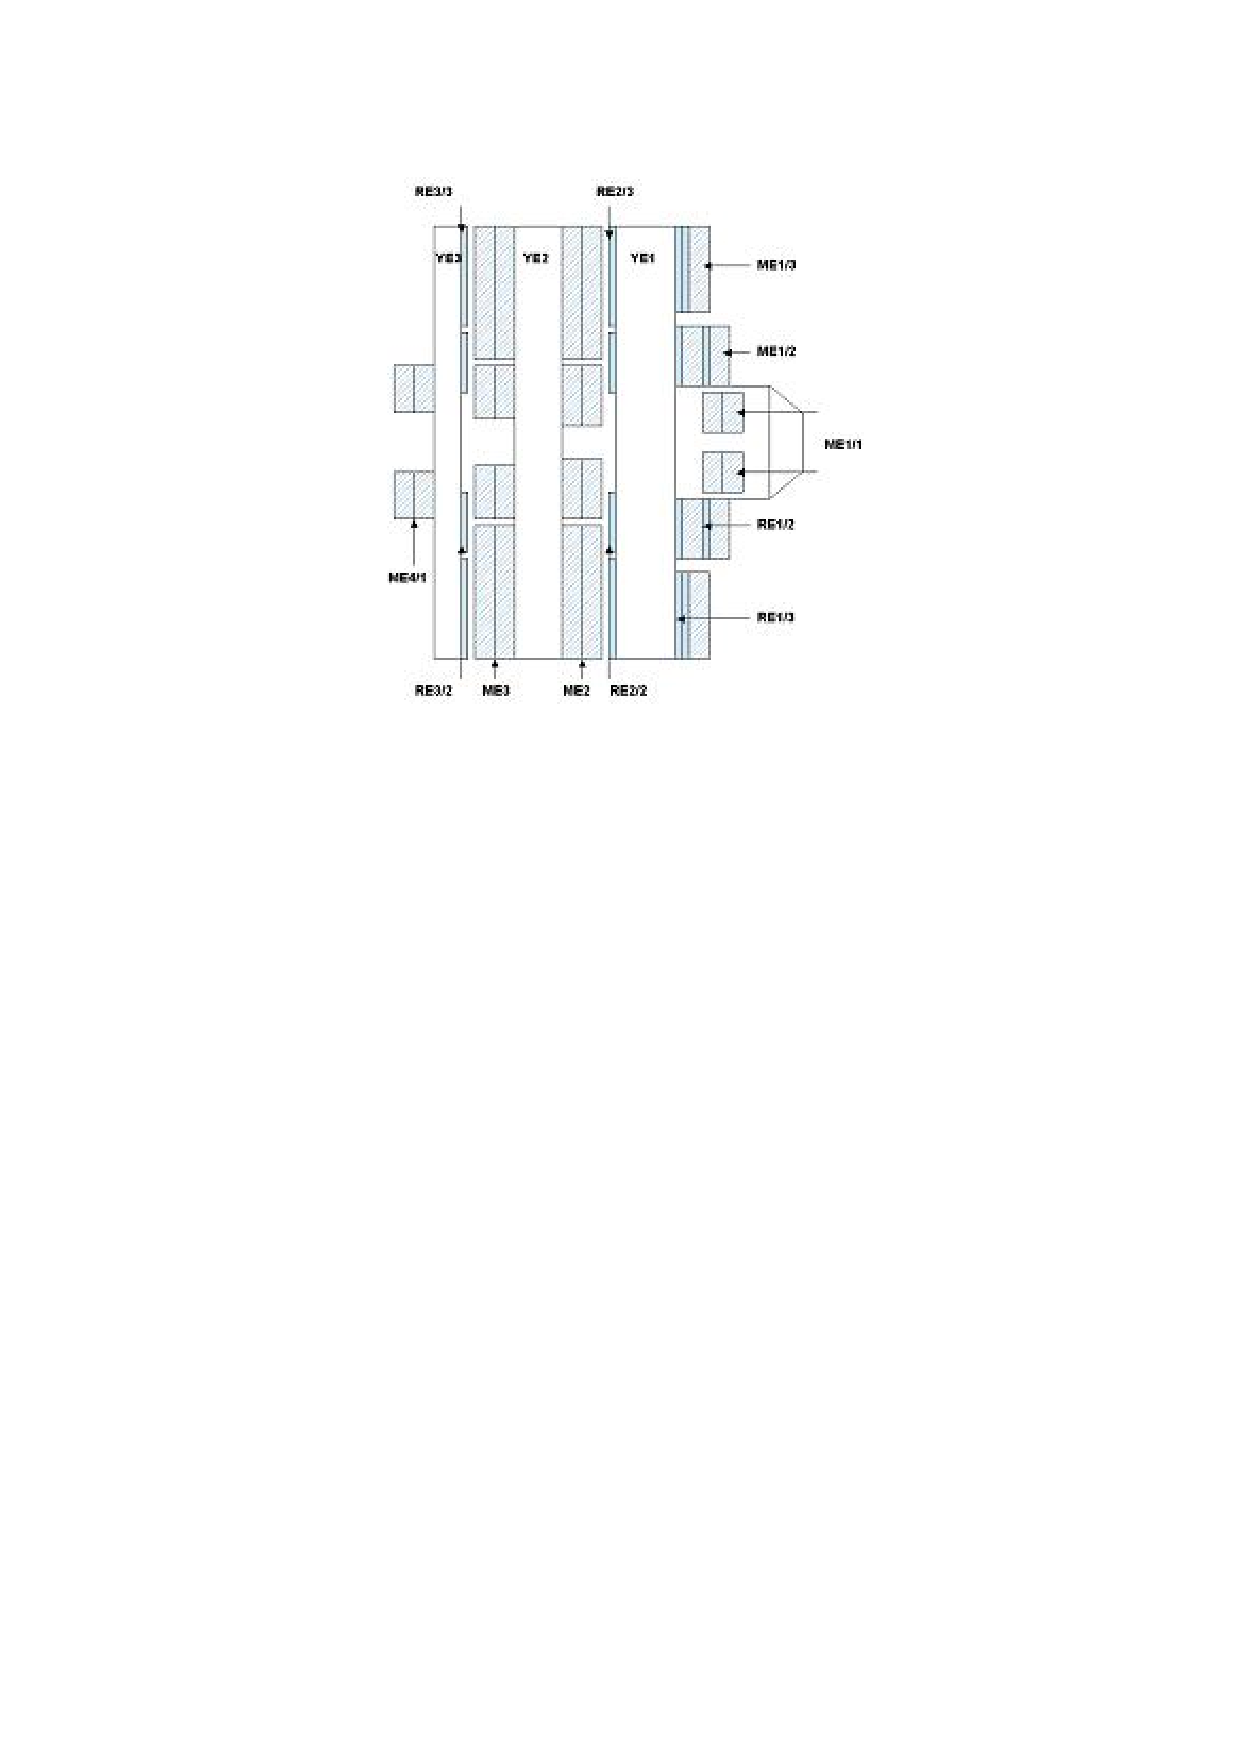
\includegraphics[width=\cmsFigWidth]{figures/cms-muon-RPCendcaplayout}
    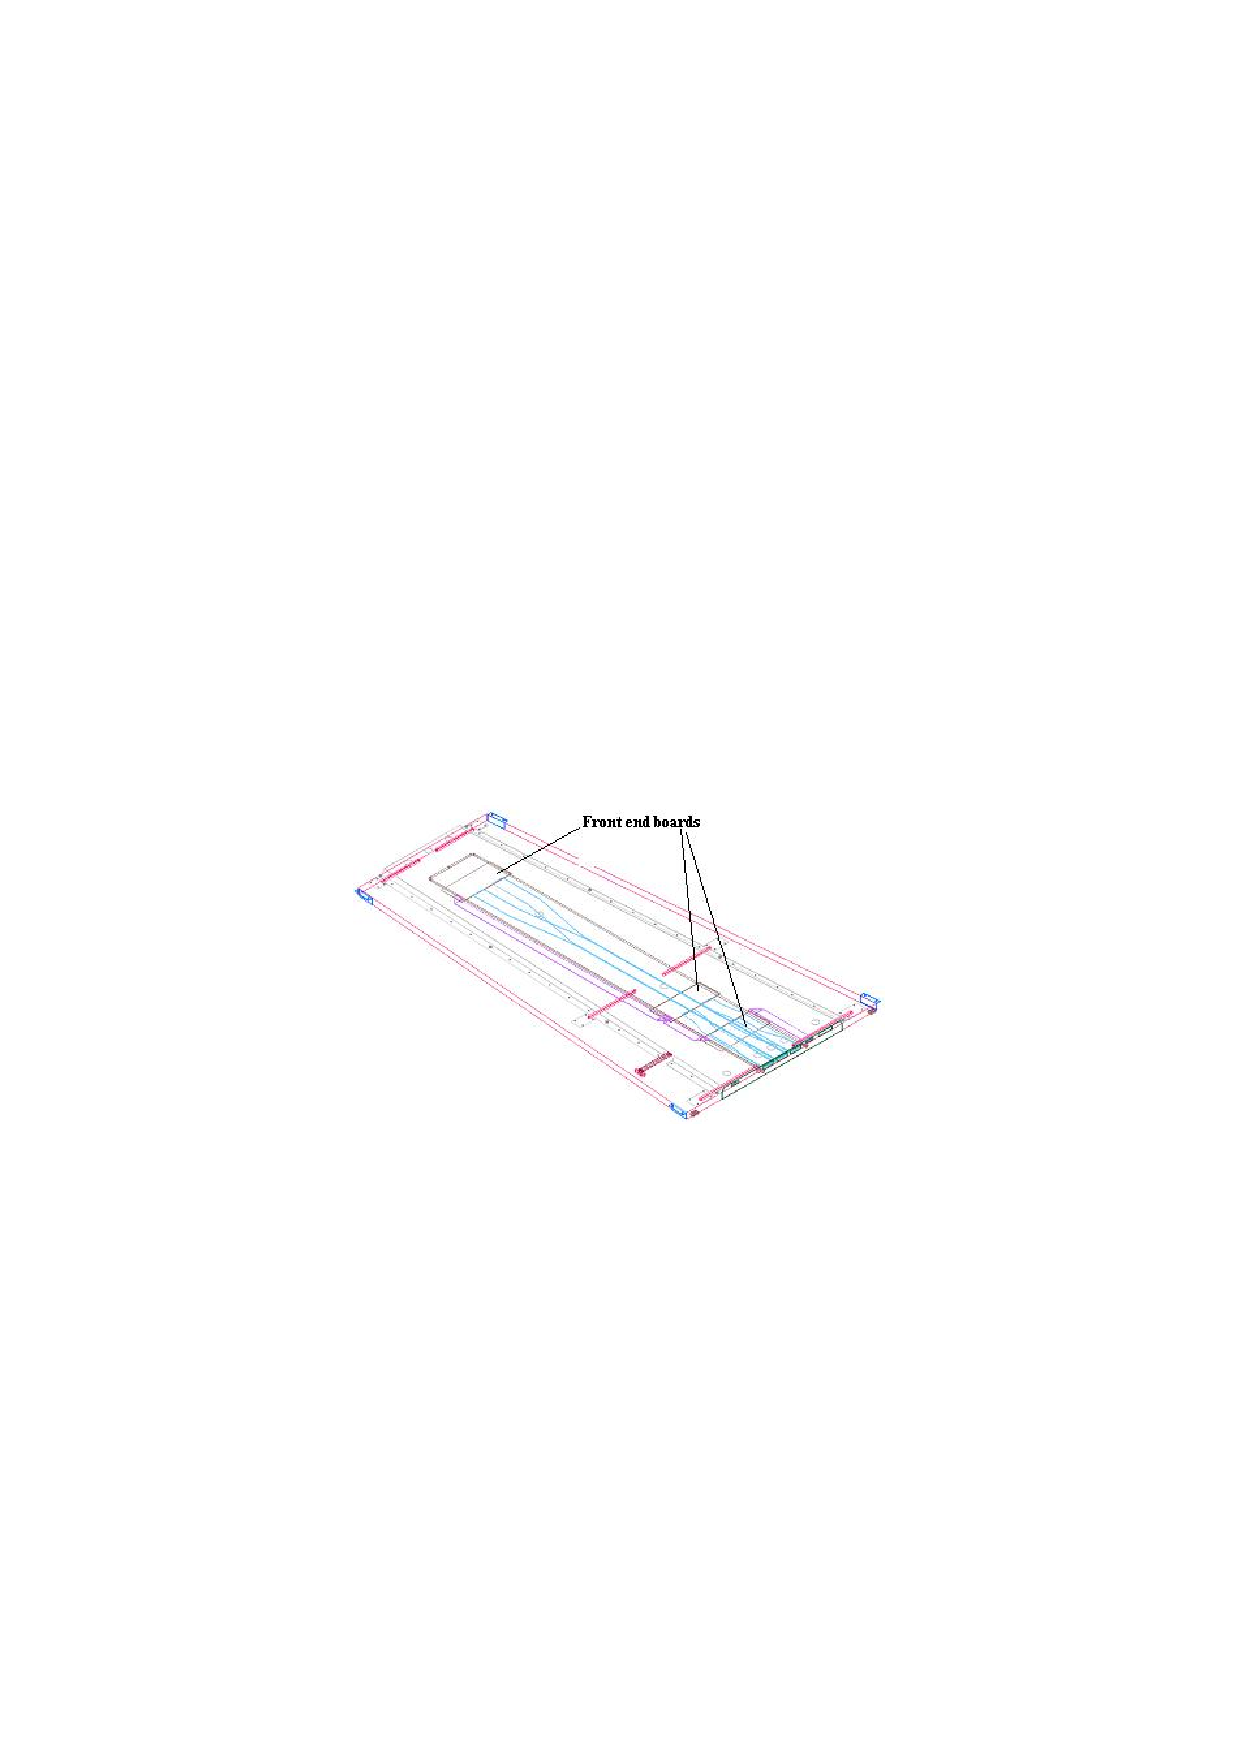
\includegraphics[width=\cmsFigWidth]{figures/cms-muon-RPCendcapchamber}
    \caption{(\cmsLeft) Layout of the RPC endcap. (\cmsRight) Endcap RPC chamber.~\cite{1748-0221-3-08-S08004}}
    \label{fig:cms-muon-RPCendcap}
  \end{center}
\end{figure}

Finally, there is the RPC system, which consists of gaseous parallel-plate detectors arranged into six barrel layers and three layers per endcap. The gas used in the chambers is a mixture of C$_2$H$_2$F$_4$, $i$C$_4$H$_{10}$, and SF$_6$ in a ratio of 96.2\%:3.5\%:0.3\%, with water vapour added to achieve 45\% relative humidity in order to avoid changes in the resistivity of the bakelite plates. The six RPC barrel layers (see schematic layout in Figure~\ref{fig:cms-muon-CSClayout}) are embedded in the iron yoke, with two in each of the first and second muon stations and one in each of the third and fourth stations. With the current endcaps, the RPC system extends out to $\abs{\eta}$ = 1.6, with future plans to install an additional fourth endcap layer that would provide coverage out to $\abs{\eta}$ = 2.1.

An RPC chamber in the barrel has a rectangular shape and consists of 2 or 3 double-gap modules with up to 96 strips per double-gap, in which the strips run parallel to the beam direction; there are a total of 480 barrel chambers. In the endcap, chambers also have a double-gap structure but are trapezoidal in shape; each chamber has 32 strips running radially and covers 20$^{\circ}$ in $\phi$ in the innermost ring and 10$^{\circ}$ in $\phi$ in the outermost ring. Figure~\ref{fig:cms-muon-RPCbarrel} shows the arrangement of the barrel RPCs in the iron yoke, as well as an example diagram of a 3-gap barrel RPC module. Figure~\ref{fig:cms-muon-RPCendcap} shows an analogous layout of the RPC endcap system, and a diagram of a typical RPC chamber.

Front-end electronics boards are always located at the strip end of both barrel and endcap chambers, to minimize the signal arrival time with respect to the interaction point. The RPCs provide timing resolution on the order of less than the 25 ns between bunch crossings, allowing the precise assignment of muon tracks to bunch crossings as well as transverse momentum measurement.

\begin{figure}[hbtp]
  \begin{center}
    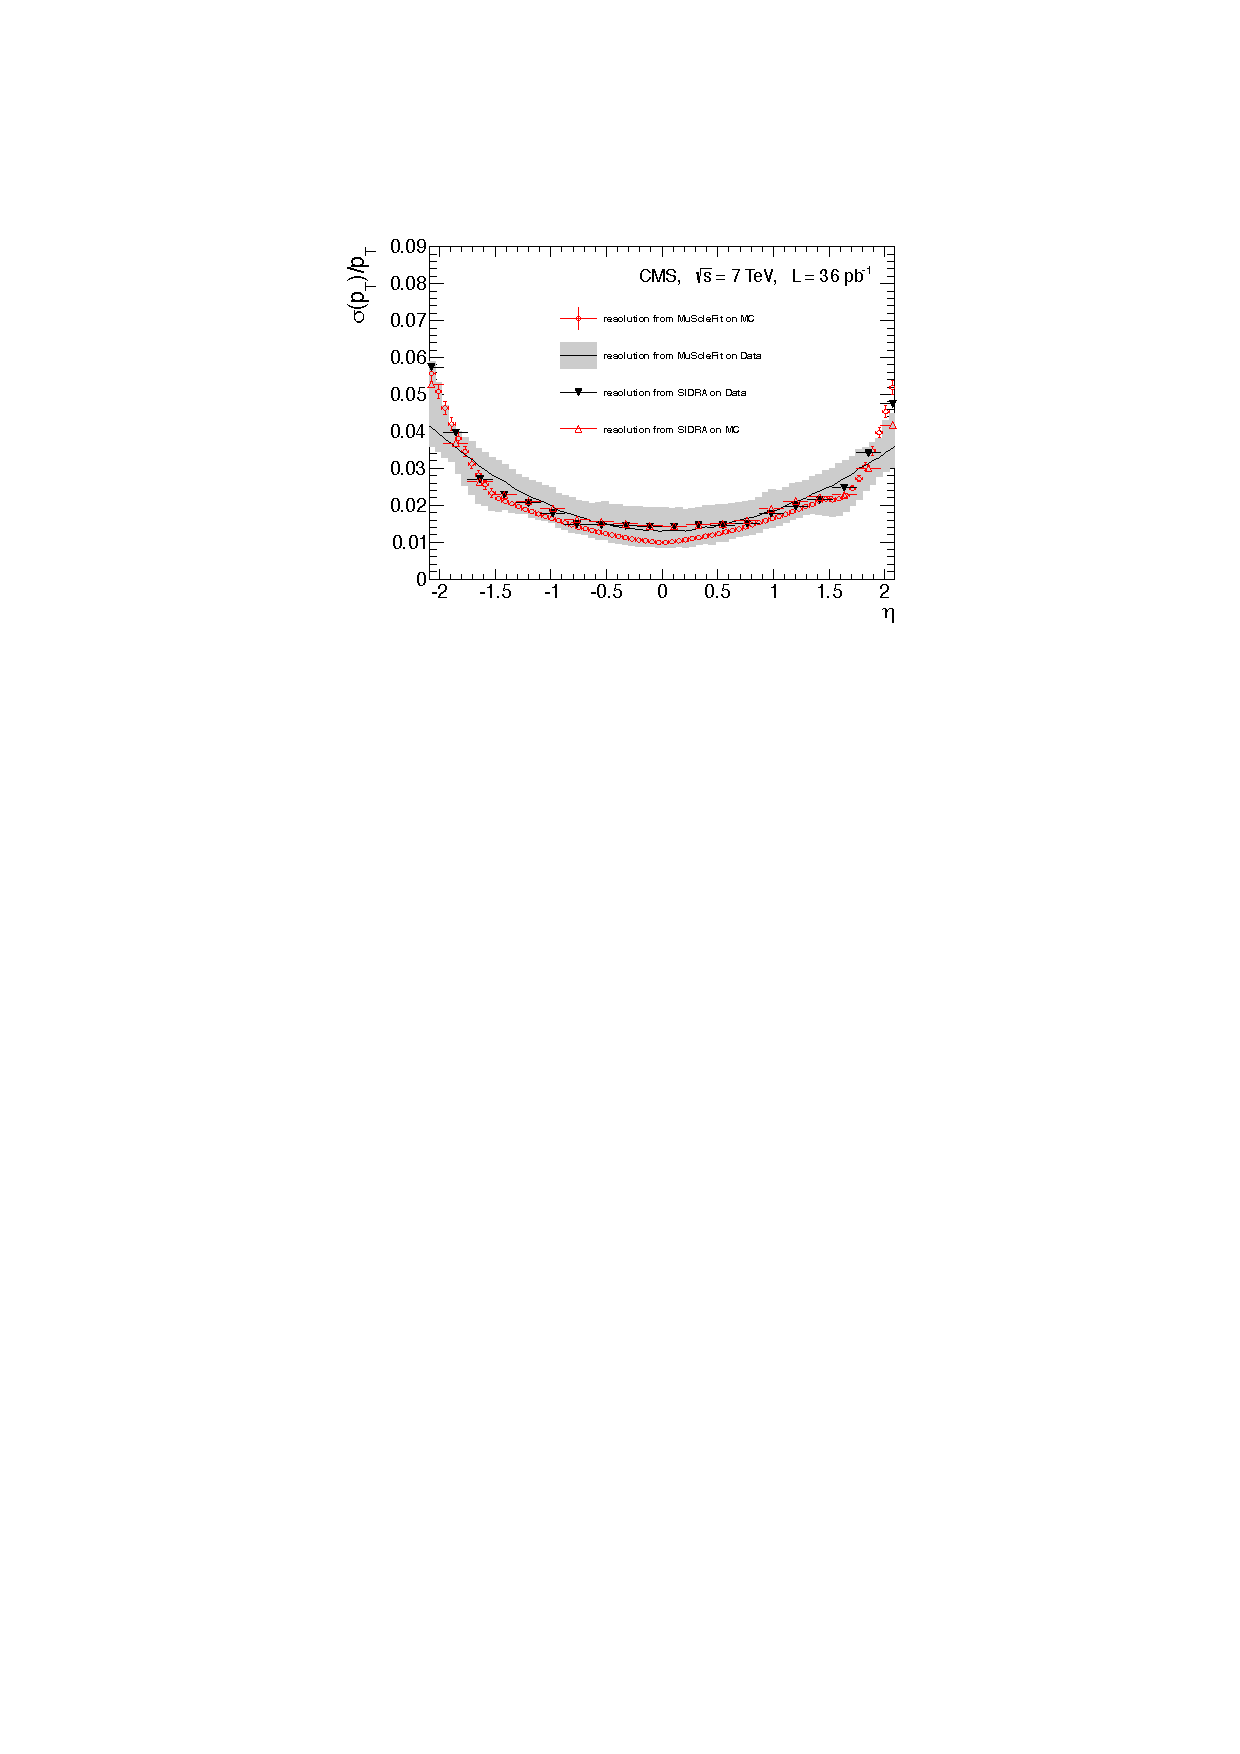
\includegraphics[width=2.0\cmsFigWidth]{figures/cms-muon-performance-Z}
    \caption{Relative $p_T$ resolution for muons from $Z$ decays, measured in 7 TeV LHC data (black curves) and in MC events (red curves), using two different algorithms, MuScleFit and SIDRA~\cite{Chatrchyan:2012xi}.}
    \label{fig:cms-muon-performance}
  \end{center}
\end{figure}

All in all, the muon system achieves a high relative $p_T$ resolution, measuring 1.3-2.0\% in the barrel and less than 6\% in the endcaps~\cite{Chatrchyan:2012xi}. The results of a study done in 7-TeV data and MC events are displayed in Figure~\ref{fig:cms-muon-performance}; in this plot of relative muon $p_T$ resolution versus $\eta$, the relative $p_T$ resolution is shown not to exceed 6\%.

\section{Triggering and data acquisition\label{sec:cms-triggerdaq}}
% rationale, L1, HLT; muon, calorimeter, global
Every collision of proton bunches at the CMS interaction points produces a large number of particles traversing the volume of the CMS detector. With protons colliding in the LHC tunnel at a rate of 40 MHz (1 bunch crossing every 25 ns) and about 20 proton-proton collisions per bunch crossing at the design luminosity of 10$^{34}$ cm$^{-2}$s$^{-1}$, a huge amount of data is generated at a high frequency. In order to save information from only the most important events and thus respect the limitations of the electronics and computer systems that process and store this data, a method for drastically reducing the rate of data acquisition is required. The trigger system of the CMS experiment performs a rapid assessment of each event recorded, storing the data from the event only if it passes certain criteria that mark it as an event of interest. Triggering is performed in two main steps, the Level 1 (L1) Trigger and the High Level Trigger (HLT). Together, these two steps provide a combined rate reduction factor of at least 10$^6$.

\begin{figure}[hbtp]
  \begin{center}
    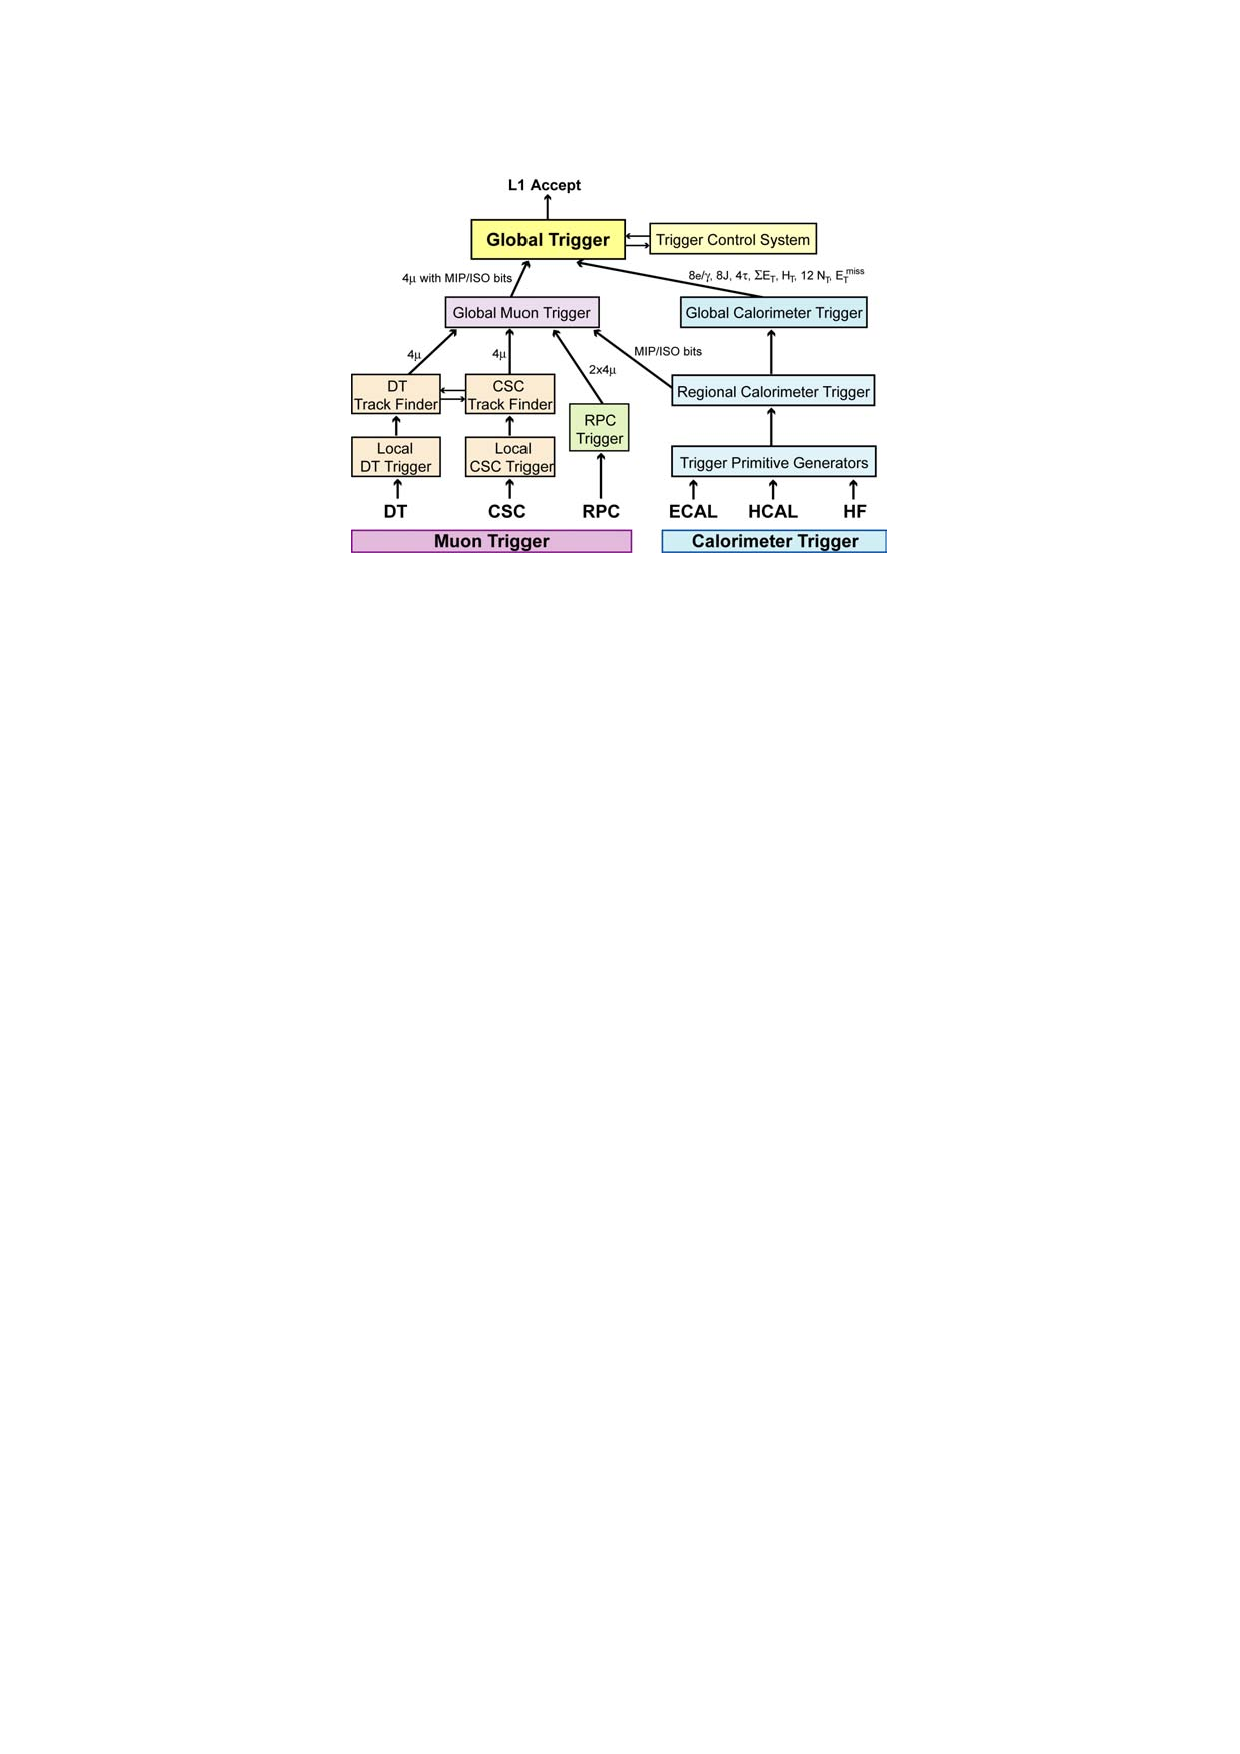
\includegraphics[width=1.5\cmsFigWidth]{figures/cms-L1flowchart}
    \caption{Flowchart of the steps and components in the L1 Trigger sequence~\cite{1748-0221-3-08-S08004}.}
    \label{fig:cms-L1flowchart}
  \end{center}
\end{figure}

The L1 Trigger consists of a system of programmable electronics, located partly in the CMS detector and partly in the underground control room near the experimental cavern. Energy deposits in calorimeter trigger towers serve as input to the local calorimeter trigger component of the L1, while track segments and hit patterns from the muon chamber serve as input to the local muon trigger component. Regional calorimeter triggers and DT and CSC track finders take the information from the local triggers and search for patterns in order to rank and sort trigger objects based on their energy or momentum and quality. Next, the global calorimeter trigger and global muon trigger take the output of their respective regional triggers and pick out the highest-ranking calorimeter and muon objects across the whole experiment. This information is finally passed to the global trigger at the end of the L1 decision chain, which uses various algorithm calculations to assess whether to reject the event completely or to accept it to be passed on to the HLT; if the event passes the L1 criteria and all the subdetectors and data acquisition (DAQ) systems are ready, then the event data are passed to the HLT.

The above steps are illustrated by the flowchart in Figure~\ref{fig:cms-L1flowchart}. The L1 Trigger analyzes every bunch crossing, with a latency period of 3.2 $\mu$s between one bunch crossing and the distribution of the trigger decision to the front-end electronics. Its design output rate limit without data recording is 100 kHz; in practice, the final rate is on the order of 30 kHz.

\begin{figure}[hbtp]
  \begin{center}
    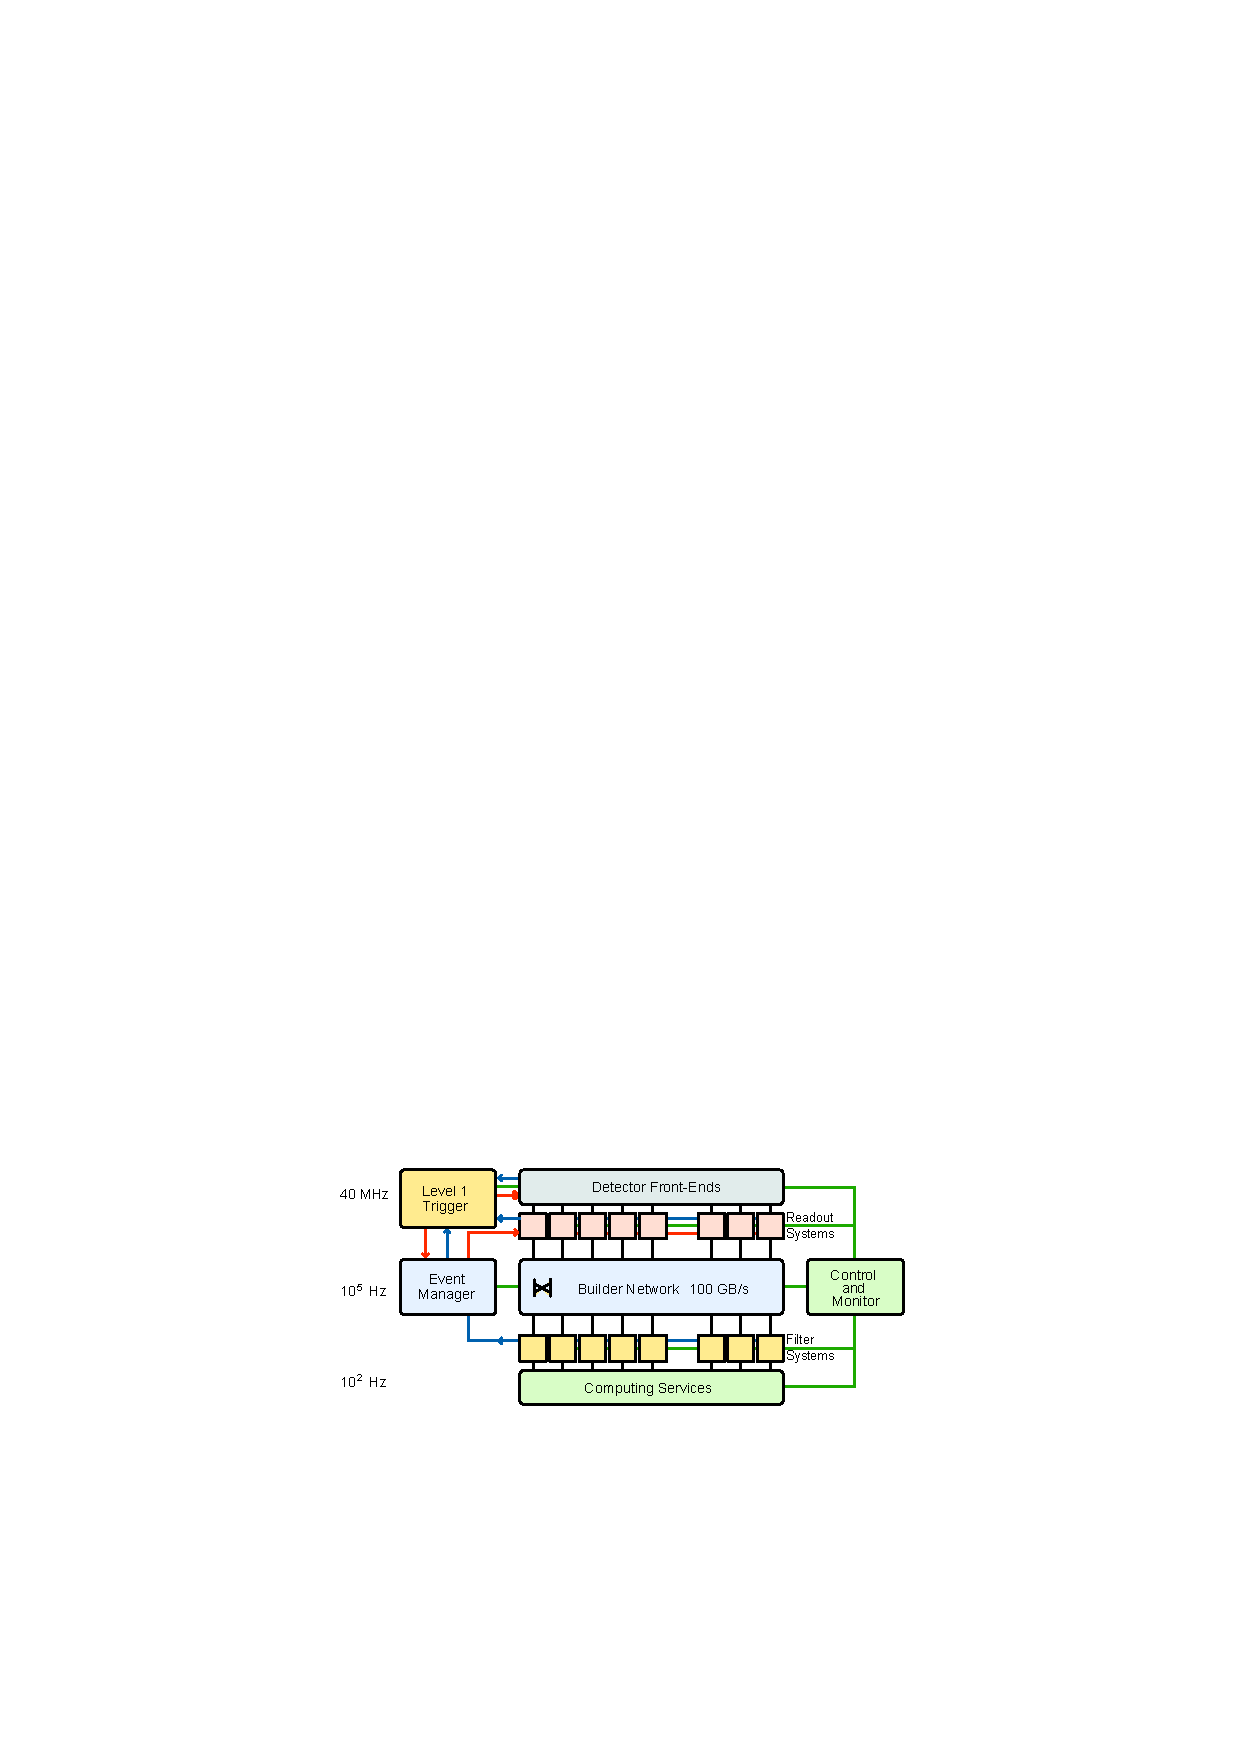
\includegraphics[width=1.5\cmsFigWidth]{figures/cms-DAQflowchart}
    \caption{Flowchart of the CMS DAQ architecture~\cite{1748-0221-3-08-S08004}.}
    \label{fig:cms-DAQflowchart}
  \end{center}
\end{figure}

When an event passes the L1 Trigger, the data is passed to the CMS DAQ system, which is schematically depicted in Figure~\ref{fig:cms-DAQflowchart}. The subdetector front-end systems store event data in buffers until the L1 Trigger decision allows them to release this data to the front-end drivers (FEDs) of the DAQ system. Event fragments from the FEDs are merged by a set of processors called the Event Builder to produce a data structure containing the complete event information, which is then passed to the Event Filter, a computer farm of about one thousand PC's. The Event Filter submits the event data to the HLT, a flexible software system implemented in the computers of the Event Filter, and also performs data quality monitoring (DQM) to assess the goodness of the data.

The HLT~\cite{Cittolin:578006} runs reconstruction and filtering algorithms on the event data. The reconstruction process builds physics objects (C++ data structures) from the raw data using a streamlined version of the CMS offline reconstruction software (which is described later in Section~\ref{sec:cms-reco}. The filtering process selects whether or not to keep an event, based on the criteria that classify it as having interesting physics content; these criteria define what is known as the HLT path, and they vary widely depending on the physics object or combinations of objects being selected. Many different HLT paths are used for the numerous physics searches carried out by the CMS experiment. One example of an HLT path is a single-muon trigger that stores events if they contain at least one muon with $p_T$ $>$ 24 GeV and whose isolation -- measured by summing the pixel tracks and calorimeter energy deposits in a cone of fixed radius about the direction of the muon's reconstructed four-momentum -- is lower than some maximum cutoff. Other examples of HLT paths include selections on the $p_T$, isolation, and multiplicity of electrons and muons, the energy and multiplicity of jets, and the amount of missing transverse energy in an event.

From the input rate of around 100 kHz from the L1 Trigger, the HLT ultimately reduces the rate of event processing to $\mathcal{O}$(100) Hz. Datasets of raw events passing the HLT are written to permanent storage and undergo further offline processing before they are ready for use in physics studies or for calibration and data monitoring.

\section{Luminosity measurement\label{sec:cms-lumi}}
% HF and pixel methods

The CMS experiment has two different systems for measuring the luminosity delivered by the LHC. One relies on the forward calorimeter HF, while the other uses the pixel detector~\cite{CMS-PAS-LUM-13-001}. These two methods have different strengths and can be used as cross-checks for one another.

The HF zero counting method calculates the average luminosity per bunch crossing to 1\% statistical accuracy by estimating the mean number of interactions per bunch crossing from the average number of empty HF towers. Because of its high accuracy and the fact that HF can operate even during unstable beam conditions, the official online luminosity measurement (i.e., measured while the detector is running) during Run I has been taken from the HF zero counting method. Figure~\ref{fig:cms-lumi2012} shows a plot of the total integrated luminosity per day delivered by the LHC and recorded by CMS during the proton-proton collisions at center-of-mass energy 8 TeV during the year 2012.

\begin{figure}[hbtp]
  \begin{center}
    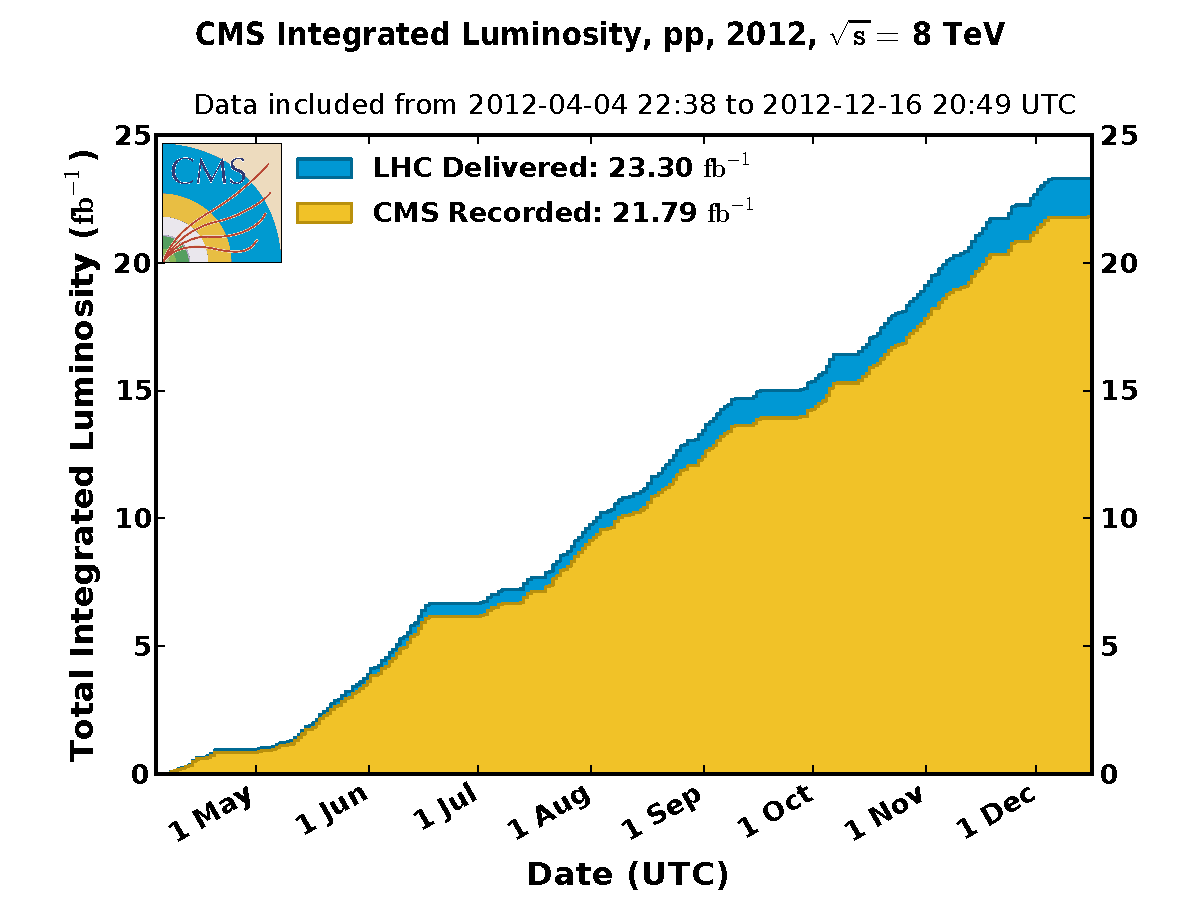
\includegraphics[width=1.5\cmsFigWidth]{figures/cms-lumi2012}
    \caption{Total integrated luminosity per day delivered by the LHC (blue) and recorded by CMS (yellow) for proton-proton collisions at 8 TeV in 2012~\cite{CMS-total-lumi}.}
    \label{fig:cms-lumi2012}
  \end{center}
\end{figure}

Offline measurements of luminosity are performed using information from the pixel system, which can only operate during stable beam conditions. The pixel-cluster counting method uses the average number of pixel clusters in a bunch crossing to calculate the instantaneous luminosity per bunch $L$ according to this formula:

\begin{equation}
L = \frac{\nu<n>}{\sigma_{vis}}
\label{eq:luminositycalculation}
\end{equation}
where $\nu =$ 11246 Hz is the beam frequency, $<n>$ is the average number of pixel clusters per event, and $\sigma_{vis}$ is the visible cross-section for inelastic collisions. $\sigma_{vis}$ is calibrated via the Van der Meer scan technique, in which the two LHC beams are scanned across each other along the horizontal and vertical planes to measure the shape and overlap of the beams. Unlike the HF-based luminosity measurement, which is susceptible to calibration drifts due to various factors, such as changes in the PMT gains and the HF detector's nonlinear response with respect to pileup, the pixel-based luminosity measurement is stable over time. Figure~\ref{fig:cms-lumipileup} illustrates the stability of the luminosity measurement as a function of pileup.

\begin{figure}[hbtp]
  \begin{center}
    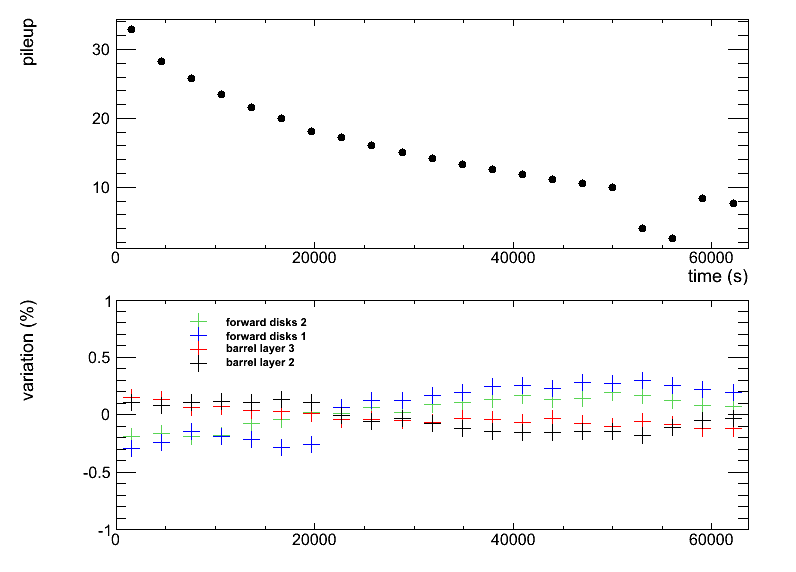
\includegraphics[width=1.5\cmsFigWidth]{figures/cms-lumipileup}
    \caption{(Top) Average rate of pileup events as a function of time during an LHC proton beam fill in November 2012. The dip towards the end is due to an end-of-fill Van der Meer scan. (Bottom) Percent variation in luminosity measurement as a function of time (or pileup), showing stable behaviour as the variation is bounded between $\pm$0.5\% over the fill period for all layers and disks of the pixel system.~\cite{CMS-total-lumi}.}
    \label{fig:cms-lumipileup}
  \end{center}
\end{figure}